%----------------------------------------------------------------------------------------
%	PACKAGES AND OTHER DOCUMENT CONFIGURATIONS
%----------------------------------------------------------------------------------------

\documentclass[
11pt, % The default document font size, options: 10pt, 11pt, 12pt
%oneside, % Two side (alternating margins) for binding by default, uncomment to switch to one side
francais, % ngerman for German
singlespacing, % Single line spacing, alternatives: onehalfspacing or doublespacing
%draft, % Uncomment to enable draft mode (no pictures, no links, overfull hboxes indicated)
%nolistspacing, % If the document is onehalfspacing or doublespacing, uncomment this to set spacing in lists to single
%liststotoc, % Uncomment to add the list of figures/tables/etc to the table of contents
%toctotoc, % Uncomment to add the main table of contents to the table of contents
%parskip, % Uncomment to add space between paragraphs
%nohyperref, % Uncomment to not load the hyperref package
headsepline, % Uncomment to get a line under the header
%chapterinoneline, % Uncomment to place the chapter title next to the number on one line
%consistentlayout, % Uncomment to change the layout of the declaration, abstract and acknowledgements pages to match the default layout
]{MastersDoctoralThesis} % The class file specifying the document structure


    \usepackage[breakable]{tcolorbox}
    \usepackage{parskip} % Stop auto-indenting (to mimic markdown behaviour)
    
    \usepackage{iftex}
    \ifPDFTeX
    	\usepackage[T1]{fontenc}
    	\usepackage{mathpazo}
    \else
    	\usepackage{fontspec}
    \fi

    % Basic figure setup, for now with no caption control since it's done
    % automatically by Pandoc (which extracts ![](path) syntax from Markdown).
    \usepackage{graphicx}
    % Maintain compatibility with old templates. Remove in nbconvert 6.0
    \let\Oldincludegraphics\includegraphics
    % Ensure that by default, figures have no caption (until we provide a
    % proper Figure object with a Caption API and a way to capture that
    % in the conversion process - todo).
    \usepackage{caption}
    \DeclareCaptionFormat{nocaption}{}
    \captionsetup{format=nocaption,aboveskip=0pt,belowskip=0pt}

    \usepackage{float}
    \floatplacement{figure}{H} % forces figures to be placed at the correct location
    \usepackage{xcolor} % Allow colors to be defined
    \usepackage{enumerate} % Needed for markdown enumerations to work
    \usepackage{geometry} % Used to adjust the document margins
    \usepackage{amsmath} % Equations
    \usepackage{amssymb} % Equations
    \usepackage{textcomp} % defines textquotesingle
    % Hack from http://tex.stackexchange.com/a/47451/13684:
    \AtBeginDocument{%
        \def\PYZsq{\textquotesingle}% Upright quotes in Pygmentized code
    }
    \usepackage{upquote} % Upright quotes for verbatim code
    \usepackage{eurosym} % defines \euro
    \usepackage[mathletters]{ucs} % Extended unicode (utf-8) support
    \usepackage{fancyvrb} % verbatim replacement that allows latex
    \usepackage{grffile} % extends the file name processing of package graphics 
                         % to support a larger range
    \makeatletter % fix for old versions of grffile with XeLaTeX
    \@ifpackagelater{grffile}{2019/11/01}
    {
      % Do nothing on new versions
    }
    {
      \def\Gread@@xetex#1{%
        \IfFileExists{"\Gin@base".bb}%
        {\Gread@eps{\Gin@base.bb}}%
        {\Gread@@xetex@aux#1}%
      }
    }
    \makeatother
    \usepackage[Export]{adjustbox} % Used to constrain images to a maximum size
    \adjustboxset{max size={0.9\linewidth}{0.9\paperheight}}

    % The hyperref package gives us a pdf with properly built
    % internal navigation ('pdf bookmarks' for the table of contents,
    % internal cross-reference links, web links for URLs, etc.)
    \usepackage{hyperref}
    % The default LaTeX title has an obnoxious amount of whitespace. By default,
    % titling removes some of it. It also provides customization options.
    \usepackage{titling}
    \usepackage{longtable} % longtable support required by pandoc >1.10
    \usepackage{booktabs}  % table support for pandoc > 1.12.2
    \usepackage[inline]{enumitem} % IRkernel/repr support (it uses the enumerate* environment)
    \usepackage[normalem]{ulem} % ulem is needed to support strikethroughs (\sout)
                                % normalem makes italics be italics, not underlines
    \usepackage{mathrsfs}
    

    
    % Colors for the hyperref package
    \definecolor{urlcolor}{rgb}{0,.145,.698}
    \definecolor{linkcolor}{rgb}{.71,0.21,0.01}
    \definecolor{citecolor}{rgb}{.12,.54,.11}

    % ANSI colors
    \definecolor{ansi-black}{HTML}{3E424D}
    \definecolor{ansi-black-intense}{HTML}{282C36}
    \definecolor{ansi-red}{HTML}{E75C58}
    \definecolor{ansi-red-intense}{HTML}{B22B31}
    \definecolor{ansi-green}{HTML}{00A250}
    \definecolor{ansi-green-intense}{HTML}{007427}
    \definecolor{ansi-yellow}{HTML}{DDB62B}
    \definecolor{ansi-yellow-intense}{HTML}{B27D12}
    \definecolor{ansi-blue}{HTML}{208FFB}
    \definecolor{ansi-blue-intense}{HTML}{0065CA}
    \definecolor{ansi-magenta}{HTML}{D160C4}
    \definecolor{ansi-magenta-intense}{HTML}{A03196}
    \definecolor{ansi-cyan}{HTML}{60C6C8}
    \definecolor{ansi-cyan-intense}{HTML}{258F8F}
    \definecolor{ansi-white}{HTML}{C5C1B4}
    \definecolor{ansi-white-intense}{HTML}{A1A6B2}
    \definecolor{ansi-default-inverse-fg}{HTML}{FFFFFF}
    \definecolor{ansi-default-inverse-bg}{HTML}{000000}

    % common color for the border for error outputs.
    \definecolor{outerrorbackground}{HTML}{FFDFDF}

    % commands and environments needed by pandoc snippets
    % extracted from the output of `pandoc -s`
    \providecommand{\tightlist}{%
      \setlength{\itemsep}{0pt}\setlength{\parskip}{0pt}}
    \DefineVerbatimEnvironment{Highlighting}{Verbatim}{commandchars=\\\{\}}
    % Add ',fontsize=\small' for more characters per line
    \newenvironment{Shaded}{}{}
    \newcommand{\KeywordTok}[1]{\textcolor[rgb]{0.00,0.44,0.13}{\textbf{{#1}}}}
    \newcommand{\DataTypeTok}[1]{\textcolor[rgb]{0.56,0.13,0.00}{{#1}}}
    \newcommand{\DecValTok}[1]{\textcolor[rgb]{0.25,0.63,0.44}{{#1}}}
    \newcommand{\BaseNTok}[1]{\textcolor[rgb]{0.25,0.63,0.44}{{#1}}}
    \newcommand{\FloatTok}[1]{\textcolor[rgb]{0.25,0.63,0.44}{{#1}}}
    \newcommand{\CharTok}[1]{\textcolor[rgb]{0.25,0.44,0.63}{{#1}}}
    \newcommand{\StringTok}[1]{\textcolor[rgb]{0.25,0.44,0.63}{{#1}}}
    \newcommand{\CommentTok}[1]{\textcolor[rgb]{0.38,0.63,0.69}{\textit{{#1}}}}
    \newcommand{\OtherTok}[1]{\textcolor[rgb]{0.00,0.44,0.13}{{#1}}}
    \newcommand{\AlertTok}[1]{\textcolor[rgb]{1.00,0.00,0.00}{\textbf{{#1}}}}
    \newcommand{\FunctionTok}[1]{\textcolor[rgb]{0.02,0.16,0.49}{{#1}}}
    \newcommand{\RegionMarkerTok}[1]{{#1}}
    \newcommand{\ErrorTok}[1]{\textcolor[rgb]{1.00,0.00,0.00}{\textbf{{#1}}}}
    \newcommand{\NormalTok}[1]{{#1}}
    
    % Additional commands for more recent versions of Pandoc
    \newcommand{\ConstantTok}[1]{\textcolor[rgb]{0.53,0.00,0.00}{{#1}}}
    \newcommand{\SpecialCharTok}[1]{\textcolor[rgb]{0.25,0.44,0.63}{{#1}}}
    \newcommand{\VerbatimStringTok}[1]{\textcolor[rgb]{0.25,0.44,0.63}{{#1}}}
    \newcommand{\SpecialStringTok}[1]{\textcolor[rgb]{0.73,0.40,0.53}{{#1}}}
    \newcommand{\ImportTok}[1]{{#1}}
    \newcommand{\DocumentationTok}[1]{\textcolor[rgb]{0.73,0.13,0.13}{\textit{{#1}}}}
    \newcommand{\AnnotationTok}[1]{\textcolor[rgb]{0.38,0.63,0.69}{\textbf{\textit{{#1}}}}}
    \newcommand{\CommentVarTok}[1]{\textcolor[rgb]{0.38,0.63,0.69}{\textbf{\textit{{#1}}}}}
    \newcommand{\VariableTok}[1]{\textcolor[rgb]{0.10,0.09,0.49}{{#1}}}
    \newcommand{\ControlFlowTok}[1]{\textcolor[rgb]{0.00,0.44,0.13}{\textbf{{#1}}}}
    \newcommand{\OperatorTok}[1]{\textcolor[rgb]{0.40,0.40,0.40}{{#1}}}
    \newcommand{\BuiltInTok}[1]{{#1}}
    \newcommand{\ExtensionTok}[1]{{#1}}
    \newcommand{\PreprocessorTok}[1]{\textcolor[rgb]{0.74,0.48,0.00}{{#1}}}
    \newcommand{\AttributeTok}[1]{\textcolor[rgb]{0.49,0.56,0.16}{{#1}}}
    \newcommand{\InformationTok}[1]{\textcolor[rgb]{0.38,0.63,0.69}{\textbf{\textit{{#1}}}}}
    \newcommand{\WarningTok}[1]{\textcolor[rgb]{0.38,0.63,0.69}{\textbf{\textit{{#1}}}}}
    
    
    % Define a nice break command that doesn't care if a line doesn't already
    % exist.
    \def\br{\hspace*{\fill} \\* }
    % Math Jax compatibility definitions
    \def\gt{>}
    \def\lt{<}
    \let\Oldtex\TeX
    \let\Oldlatex\LaTeX
    \renewcommand{\TeX}{\textrm{\Oldtex}}
    \renewcommand{\LaTeX}{\textrm{\Oldlatex}}
    % Document parameters
    % Document title
    \title{Implementation\_1D\_Fond}
    
    
    
    
    
% Pygments definitions
\makeatletter
\def\PY@reset{\let\PY@it=\relax \let\PY@bf=\relax%
    \let\PY@ul=\relax \let\PY@tc=\relax%
    \let\PY@bc=\relax \let\PY@ff=\relax}
\def\PY@tok#1{\csname PY@tok@#1\endcsname}
\def\PY@toks#1+{\ifx\relax#1\empty\else%
    \PY@tok{#1}\expandafter\PY@toks\fi}
\def\PY@do#1{\PY@bc{\PY@tc{\PY@ul{%
    \PY@it{\PY@bf{\PY@ff{#1}}}}}}}
\def\PY#1#2{\PY@reset\PY@toks#1+\relax+\PY@do{#2}}

\@namedef{PY@tok@w}{\def\PY@tc##1{\textcolor[rgb]{0.73,0.73,0.73}{##1}}}
\@namedef{PY@tok@c}{\let\PY@it=\textit\def\PY@tc##1{\textcolor[rgb]{0.25,0.50,0.50}{##1}}}
\@namedef{PY@tok@cp}{\def\PY@tc##1{\textcolor[rgb]{0.74,0.48,0.00}{##1}}}
\@namedef{PY@tok@k}{\let\PY@bf=\textbf\def\PY@tc##1{\textcolor[rgb]{0.00,0.50,0.00}{##1}}}
\@namedef{PY@tok@kp}{\def\PY@tc##1{\textcolor[rgb]{0.00,0.50,0.00}{##1}}}
\@namedef{PY@tok@kt}{\def\PY@tc##1{\textcolor[rgb]{0.69,0.00,0.25}{##1}}}
\@namedef{PY@tok@o}{\def\PY@tc##1{\textcolor[rgb]{0.40,0.40,0.40}{##1}}}
\@namedef{PY@tok@ow}{\let\PY@bf=\textbf\def\PY@tc##1{\textcolor[rgb]{0.67,0.13,1.00}{##1}}}
\@namedef{PY@tok@nb}{\def\PY@tc##1{\textcolor[rgb]{0.00,0.50,0.00}{##1}}}
\@namedef{PY@tok@nf}{\def\PY@tc##1{\textcolor[rgb]{0.00,0.00,1.00}{##1}}}
\@namedef{PY@tok@nc}{\let\PY@bf=\textbf\def\PY@tc##1{\textcolor[rgb]{0.00,0.00,1.00}{##1}}}
\@namedef{PY@tok@nn}{\let\PY@bf=\textbf\def\PY@tc##1{\textcolor[rgb]{0.00,0.00,1.00}{##1}}}
\@namedef{PY@tok@ne}{\let\PY@bf=\textbf\def\PY@tc##1{\textcolor[rgb]{0.82,0.25,0.23}{##1}}}
\@namedef{PY@tok@nv}{\def\PY@tc##1{\textcolor[rgb]{0.10,0.09,0.49}{##1}}}
\@namedef{PY@tok@no}{\def\PY@tc##1{\textcolor[rgb]{0.53,0.00,0.00}{##1}}}
\@namedef{PY@tok@nl}{\def\PY@tc##1{\textcolor[rgb]{0.63,0.63,0.00}{##1}}}
\@namedef{PY@tok@ni}{\let\PY@bf=\textbf\def\PY@tc##1{\textcolor[rgb]{0.60,0.60,0.60}{##1}}}
\@namedef{PY@tok@na}{\def\PY@tc##1{\textcolor[rgb]{0.49,0.56,0.16}{##1}}}
\@namedef{PY@tok@nt}{\let\PY@bf=\textbf\def\PY@tc##1{\textcolor[rgb]{0.00,0.50,0.00}{##1}}}
\@namedef{PY@tok@nd}{\def\PY@tc##1{\textcolor[rgb]{0.67,0.13,1.00}{##1}}}
\@namedef{PY@tok@s}{\def\PY@tc##1{\textcolor[rgb]{0.73,0.13,0.13}{##1}}}
\@namedef{PY@tok@sd}{\let\PY@it=\textit\def\PY@tc##1{\textcolor[rgb]{0.73,0.13,0.13}{##1}}}
\@namedef{PY@tok@si}{\let\PY@bf=\textbf\def\PY@tc##1{\textcolor[rgb]{0.73,0.40,0.53}{##1}}}
\@namedef{PY@tok@se}{\let\PY@bf=\textbf\def\PY@tc##1{\textcolor[rgb]{0.73,0.40,0.13}{##1}}}
\@namedef{PY@tok@sr}{\def\PY@tc##1{\textcolor[rgb]{0.73,0.40,0.53}{##1}}}
\@namedef{PY@tok@ss}{\def\PY@tc##1{\textcolor[rgb]{0.10,0.09,0.49}{##1}}}
\@namedef{PY@tok@sx}{\def\PY@tc##1{\textcolor[rgb]{0.00,0.50,0.00}{##1}}}
\@namedef{PY@tok@m}{\def\PY@tc##1{\textcolor[rgb]{0.40,0.40,0.40}{##1}}}
\@namedef{PY@tok@gh}{\let\PY@bf=\textbf\def\PY@tc##1{\textcolor[rgb]{0.00,0.00,0.50}{##1}}}
\@namedef{PY@tok@gu}{\let\PY@bf=\textbf\def\PY@tc##1{\textcolor[rgb]{0.50,0.00,0.50}{##1}}}
\@namedef{PY@tok@gd}{\def\PY@tc##1{\textcolor[rgb]{0.63,0.00,0.00}{##1}}}
\@namedef{PY@tok@gi}{\def\PY@tc##1{\textcolor[rgb]{0.00,0.63,0.00}{##1}}}
\@namedef{PY@tok@gr}{\def\PY@tc##1{\textcolor[rgb]{1.00,0.00,0.00}{##1}}}
\@namedef{PY@tok@ge}{\let\PY@it=\textit}
\@namedef{PY@tok@gs}{\let\PY@bf=\textbf}
\@namedef{PY@tok@gp}{\let\PY@bf=\textbf\def\PY@tc##1{\textcolor[rgb]{0.00,0.00,0.50}{##1}}}
\@namedef{PY@tok@go}{\def\PY@tc##1{\textcolor[rgb]{0.53,0.53,0.53}{##1}}}
\@namedef{PY@tok@gt}{\def\PY@tc##1{\textcolor[rgb]{0.00,0.27,0.87}{##1}}}
\@namedef{PY@tok@err}{\def\PY@bc##1{{\setlength{\fboxsep}{\string -\fboxrule}\fcolorbox[rgb]{1.00,0.00,0.00}{1,1,1}{\strut ##1}}}}
\@namedef{PY@tok@kc}{\let\PY@bf=\textbf\def\PY@tc##1{\textcolor[rgb]{0.00,0.50,0.00}{##1}}}
\@namedef{PY@tok@kd}{\let\PY@bf=\textbf\def\PY@tc##1{\textcolor[rgb]{0.00,0.50,0.00}{##1}}}
\@namedef{PY@tok@kn}{\let\PY@bf=\textbf\def\PY@tc##1{\textcolor[rgb]{0.00,0.50,0.00}{##1}}}
\@namedef{PY@tok@kr}{\let\PY@bf=\textbf\def\PY@tc##1{\textcolor[rgb]{0.00,0.50,0.00}{##1}}}
\@namedef{PY@tok@bp}{\def\PY@tc##1{\textcolor[rgb]{0.00,0.50,0.00}{##1}}}
\@namedef{PY@tok@fm}{\def\PY@tc##1{\textcolor[rgb]{0.00,0.00,1.00}{##1}}}
\@namedef{PY@tok@vc}{\def\PY@tc##1{\textcolor[rgb]{0.10,0.09,0.49}{##1}}}
\@namedef{PY@tok@vg}{\def\PY@tc##1{\textcolor[rgb]{0.10,0.09,0.49}{##1}}}
\@namedef{PY@tok@vi}{\def\PY@tc##1{\textcolor[rgb]{0.10,0.09,0.49}{##1}}}
\@namedef{PY@tok@vm}{\def\PY@tc##1{\textcolor[rgb]{0.10,0.09,0.49}{##1}}}
\@namedef{PY@tok@sa}{\def\PY@tc##1{\textcolor[rgb]{0.73,0.13,0.13}{##1}}}
\@namedef{PY@tok@sb}{\def\PY@tc##1{\textcolor[rgb]{0.73,0.13,0.13}{##1}}}
\@namedef{PY@tok@sc}{\def\PY@tc##1{\textcolor[rgb]{0.73,0.13,0.13}{##1}}}
\@namedef{PY@tok@dl}{\def\PY@tc##1{\textcolor[rgb]{0.73,0.13,0.13}{##1}}}
\@namedef{PY@tok@s2}{\def\PY@tc##1{\textcolor[rgb]{0.73,0.13,0.13}{##1}}}
\@namedef{PY@tok@sh}{\def\PY@tc##1{\textcolor[rgb]{0.73,0.13,0.13}{##1}}}
\@namedef{PY@tok@s1}{\def\PY@tc##1{\textcolor[rgb]{0.73,0.13,0.13}{##1}}}
\@namedef{PY@tok@mb}{\def\PY@tc##1{\textcolor[rgb]{0.40,0.40,0.40}{##1}}}
\@namedef{PY@tok@mf}{\def\PY@tc##1{\textcolor[rgb]{0.40,0.40,0.40}{##1}}}
\@namedef{PY@tok@mh}{\def\PY@tc##1{\textcolor[rgb]{0.40,0.40,0.40}{##1}}}
\@namedef{PY@tok@mi}{\def\PY@tc##1{\textcolor[rgb]{0.40,0.40,0.40}{##1}}}
\@namedef{PY@tok@il}{\def\PY@tc##1{\textcolor[rgb]{0.40,0.40,0.40}{##1}}}
\@namedef{PY@tok@mo}{\def\PY@tc##1{\textcolor[rgb]{0.40,0.40,0.40}{##1}}}
\@namedef{PY@tok@ch}{\let\PY@it=\textit\def\PY@tc##1{\textcolor[rgb]{0.25,0.50,0.50}{##1}}}
\@namedef{PY@tok@cm}{\let\PY@it=\textit\def\PY@tc##1{\textcolor[rgb]{0.25,0.50,0.50}{##1}}}
\@namedef{PY@tok@cpf}{\let\PY@it=\textit\def\PY@tc##1{\textcolor[rgb]{0.25,0.50,0.50}{##1}}}
\@namedef{PY@tok@c1}{\let\PY@it=\textit\def\PY@tc##1{\textcolor[rgb]{0.25,0.50,0.50}{##1}}}
\@namedef{PY@tok@cs}{\let\PY@it=\textit\def\PY@tc##1{\textcolor[rgb]{0.25,0.50,0.50}{##1}}}

\def\PYZbs{\char`\\}
\def\PYZus{\char`\_}
\def\PYZob{\char`\{}
\def\PYZcb{\char`\}}
\def\PYZca{\char`\^}
\def\PYZam{\char`\&}
\def\PYZlt{\char`\<}
\def\PYZgt{\char`\>}
\def\PYZsh{\char`\#}
\def\PYZpc{\char`\%}
\def\PYZdl{\char`\$}
\def\PYZhy{\char`\-}
\def\PYZsq{\char`\'}
\def\PYZdq{\char`\"}
\def\PYZti{\char`\~}
% for compatibility with earlier versions
\def\PYZat{@}
\def\PYZlb{[}
\def\PYZrb{]}
\makeatother


    % For linebreaks inside Verbatim environment from package fancyvrb. 
    \makeatletter
        \newbox\Wrappedcontinuationbox 
        \newbox\Wrappedvisiblespacebox 
        \newcommand*\Wrappedvisiblespace {\textcolor{red}{\textvisiblespace}} 
        \newcommand*\Wrappedcontinuationsymbol {\textcolor{red}{\llap{\tiny$\m@th\hookrightarrow$}}} 
        \newcommand*\Wrappedcontinuationindent {3ex } 
        \newcommand*\Wrappedafterbreak {\kern\Wrappedcontinuationindent\copy\Wrappedcontinuationbox} 
        % Take advantage of the already applied Pygments mark-up to insert 
        % potential linebreaks for TeX processing. 
        %        {, <, #, %, $, ' and ": go to next line. 
        %        _, }, ^, &, >, - and ~: stay at end of broken line. 
        % Use of \textquotesingle for straight quote. 
        \newcommand*\Wrappedbreaksatspecials {% 
            \def\PYGZus{\discretionary{\char`\_}{\Wrappedafterbreak}{\char`\_}}% 
            \def\PYGZob{\discretionary{}{\Wrappedafterbreak\char`\{}{\char`\{}}% 
            \def\PYGZcb{\discretionary{\char`\}}{\Wrappedafterbreak}{\char`\}}}% 
            \def\PYGZca{\discretionary{\char`\^}{\Wrappedafterbreak}{\char`\^}}% 
            \def\PYGZam{\discretionary{\char`\&}{\Wrappedafterbreak}{\char`\&}}% 
            \def\PYGZlt{\discretionary{}{\Wrappedafterbreak\char`\<}{\char`\<}}% 
            \def\PYGZgt{\discretionary{\char`\>}{\Wrappedafterbreak}{\char`\>}}% 
            \def\PYGZsh{\discretionary{}{\Wrappedafterbreak\char`\#}{\char`\#}}% 
            \def\PYGZpc{\discretionary{}{\Wrappedafterbreak\char`\%}{\char`\%}}% 
            \def\PYGZdl{\discretionary{}{\Wrappedafterbreak\char`\$}{\char`\$}}% 
            \def\PYGZhy{\discretionary{\char`\-}{\Wrappedafterbreak}{\char`\-}}% 
            \def\PYGZsq{\discretionary{}{\Wrappedafterbreak\textquotesingle}{\textquotesingle}}% 
            \def\PYGZdq{\discretionary{}{\Wrappedafterbreak\char`\"}{\char`\"}}% 
            \def\PYGZti{\discretionary{\char`\~}{\Wrappedafterbreak}{\char`\~}}% 
        } 
        % Some characters . , ; ? ! / are not pygmentized. 
        % This macro makes them "active" and they will insert potential linebreaks 
        \newcommand*\Wrappedbreaksatpunct {% 
            \lccode`\~`\.\lowercase{\def~}{\discretionary{\hbox{\char`\.}}{\Wrappedafterbreak}{\hbox{\char`\.}}}% 
            \lccode`\~`\,\lowercase{\def~}{\discretionary{\hbox{\char`\,}}{\Wrappedafterbreak}{\hbox{\char`\,}}}% 
            \lccode`\~`\;\lowercase{\def~}{\discretionary{\hbox{\char`\;}}{\Wrappedafterbreak}{\hbox{\char`\;}}}% 
            \lccode`\~`\:\lowercase{\def~}{\discretionary{\hbox{\char`\:}}{\Wrappedafterbreak}{\hbox{\char`\:}}}% 
            \lccode`\~`\?\lowercase{\def~}{\discretionary{\hbox{\char`\?}}{\Wrappedafterbreak}{\hbox{\char`\?}}}% 
            \lccode`\~`\!\lowercase{\def~}{\discretionary{\hbox{\char`\!}}{\Wrappedafterbreak}{\hbox{\char`\!}}}% 
            \lccode`\~`\/\lowercase{\def~}{\discretionary{\hbox{\char`\/}}{\Wrappedafterbreak}{\hbox{\char`\/}}}% 
            \catcode`\.\active
            \catcode`\,\active 
            \catcode`\;\active
            \catcode`\:\active
            \catcode`\?\active
            \catcode`\!\active
            \catcode`\/\active 
            \lccode`\~`\~ 	
        }
    \makeatother

    \let\OriginalVerbatim=\Verbatim
    \makeatletter
    \renewcommand{\Verbatim}[1][1]{%
        %\parskip\z@skip
        \sbox\Wrappedcontinuationbox {\Wrappedcontinuationsymbol}%
        \sbox\Wrappedvisiblespacebox {\FV@SetupFont\Wrappedvisiblespace}%
        \def\FancyVerbFormatLine ##1{\hsize\linewidth
            \vtop{\raggedright\hyphenpenalty\z@\exhyphenpenalty\z@
                \doublehyphendemerits\z@\finalhyphendemerits\z@
                \strut ##1\strut}%
        }%
        % If the linebreak is at a space, the latter will be displayed as visible
        % space at end of first line, and a continuation symbol starts next line.
        % Stretch/shrink are however usually zero for typewriter font.
        \def\FV@Space {%
            \nobreak\hskip\z@ plus\fontdimen3\font minus\fontdimen4\font
            \discretionary{\copy\Wrappedvisiblespacebox}{\Wrappedafterbreak}
            {\kern\fontdimen2\font}%
        }%
        
        % Allow breaks at special characters using \PYG... macros.
        \Wrappedbreaksatspecials
        % Breaks at punctuation characters . , ; ? ! and / need catcode=\active 	
        \OriginalVerbatim[#1,codes*=\Wrappedbreaksatpunct]%
    }
    \makeatother

    % Exact colors from NB
    \definecolor{incolor}{HTML}{303F9F}
    \definecolor{outcolor}{HTML}{D84315}
    \definecolor{cellborder}{HTML}{CFCFCF}
    \definecolor{cellbackground}{HTML}{F7F7F7}
    
    % prompt
    \makeatletter
    \newcommand{\boxspacing}{\kern\kvtcb@left@rule\kern\kvtcb@boxsep}
    \makeatother
    \newcommand{\prompt}[4]{
        {\ttfamily\llap{{\color{#2}[#3]:\hspace{3pt}#4}}\vspace{-\baselineskip}}
    }
    

    
    % Prevent overflowing lines due to hard-to-break entities
    \sloppy 
    % Setup hyperref package
    \hypersetup{
      breaklinks=true,  % so long urls are correctly broken across lines
      colorlinks=true,
      urlcolor=urlcolor,
      linkcolor=linkcolor,
      citecolor=citecolor,
      }
    % Slightly bigger margins than the latex defaults
    
    \geometry{verbose,tmargin=1in,bmargin=1in,lmargin=1in,rmargin=1in}

\usepackage[utf8]{inputenc} % Required for inputting international characters
\usepackage[T1]{fontenc} % Output font encoding for international characters

\usepackage{graphicx}
\graphicspath{ {./images/} }

\usepackage{mathpazo} % Use the Palatino font by default

\usepackage{amsmath}





\usepackage[autostyle=true]{csquotes} % Required to generate language-dependent quotes in the bibliography

%----------------------------------------------------------------------------------------
%	MARGIN SETTINGS
%----------------------------------------------------------------------------------------

\geometry{
	paper=a4paper, % Change to letterpaper for US letter
	inner=2.5cm, % Inner margin
	outer=3.8cm, % Outer margin
	bindingoffset=.5cm, % Binding offset
	top=1.5cm, % Top margin
	bottom=1.5cm, % Bottom margin
	%showframe, % Uncomment to show how the type block is set on the page
}

%----------------------------------------------------------------------------------------
%	INFORMATIONS
%----------------------------------------------------------------------------------------

\thesistitle{Approximation numérique d'ordre élevé de l'équation de Saint Venant} % Title
\supervisor{Thomas \textsc{Rey}} % Your supervisor's name, this is used in the title page, print it elsewhere with \supname
\examiner{} % Your examiner's name, this is not currently used anywhere in the template, print it elsewhere with \examname
\degree{} % Your degree name, this is used in the title page and abstract, print it elsewhere with \degreename
\author{Brice \textsc{Gonel} \\ Romain \textsc{Pinguet}} % Your name, this is used in the title page and abstract, print it elsewhere with \authorname
\addresses{} % Your address, this is not currently used anywhere in the template, print it elsewhere with \addressname

\subject{} % Your subject area, this is not currently used anywhere in the template, print it elsewhere with \subjectname
\keywords{} % Keywords for your thesis, this is not currently used anywhere in the template, print it elsewhere with \keywordnames
%\university{\href{https://www.univ-lille.fr}{Université de Lille}} % Your university's name and URL, this is used in the title page and abstract, print it elsewhere with \univname
%\department{\href{http://department.university.com}{Department or School Name}} % Your department's name and URL, this is used in the title page and abstract, print it elsewhere with \deptname
%\group{\href{http://researchgroup.university.com}{Research Group Name}} % Your research group's name and URL, this is used in the title page, print it elsewhere with \groupname
%\faculty{\href{http://faculty.university.com}{Faculty Name}} % Your faculty's name and URL, this is used in the title page and abstract, print it elsewhere with \facname

\AtBeginDocument{
\hypersetup{pdftitle=\ttitle} % Set the PDF's title to your title
\hypersetup{pdfauthor=\authorname} % Set the PDF's author to your name
\hypersetup{pdfkeywords=\keywordnames} % Set the PDF's keywords to your keywords
}


%----------------------------------------------------------------------------------------
%	Autres packages utiles 
%----------------------------------------------------------------------------------------

\usepackage{amsthm}
\newtheorem{prop}{Proposition}
\renewcommand{\thesection}{\arabic{section}}
\usepackage[utf8]{inputenc}
\usepackage[T1]{fontenc}
\usepackage{cases}
\usepackage{comment}

\theoremstyle{definition}
\newtheorem{definition}{Définition}

\begin{document}

\pagestyle{plain} % Default to the plain heading style until the thesis style is called for the body content

%----------------------------------------------------------------------------------------
%	TITLE PAGE
%----------------------------------------------------------------------------------------

\begin{titlepage}
\begin{center}

\vspace*{.06\textheight}

\textsc{\Large Mémoire de recherche}\\[0.5cm] % Thesis type

\HRule \\[0.4cm] % Horizontal line
{\huge \bfseries \ttitle\par}\vspace{0.4cm} % Thesis title
\HRule \\[1.5cm] % Horizontal line
 
\begin{minipage}[t]{0.4\textwidth}
\begin{flushleft} \large
\emph{Auteurs :}\\
\authorname % Author name - remove the \href bracket to remove the link
\end{flushleft}
\end{minipage}
\begin{minipage}[t]{0.4\textwidth}
\begin{flushright} \large
\emph{Professeur encadrant :} \\
\supname % Supervisor name - remove the \href bracket to remove the link  
\end{flushright}
\end{minipage}\\[3cm]
 
\end{center}
\end{titlepage}

%----------------------------------------------------------------------------------------
%	LIST OF CONTENTS/FIGURES/TABLES PAGES
%----------------------------------------------------------------------------------------

\tableofcontents % Prints the main table of contents

%----------------------------------------------------------------------------------------
%	CONTENU
%----------------------------------------------------------------------------------------

\newpage

Les équations de Saint-Venant modélisent le comportement d'un écoulement en eau peu profonde, comme un canal ou un bord de plage.
Ces équations, introduites à la fin des années 1880, sont extrêmement bien adaptées à modélisation et à la simulation numérique de phénomènes 
catastrophiques, comme les inondations ou les tsunamis.

\section{Description et dérivation des équations}

Ici, il s'agit  d'énoncer les équations, de décrire les différentes quantités en jeu ($h$, $u$, $q$ et $Z$)
et d'expliquer comment on peut arriver à ces équations.

\subsection{Description des équations}

Le système de Saint-Venant avec terme source (qui est aussi désigné par le nom \og équations d'écoulements en eau peu profonde  \fg{}) est le suivant :

\begin{equation} \frac{\partial h}{\partial t}(t,x)+\frac{\partial q}{\partial x}(t,x)=0 \label{sveq1} \end{equation}
\begin{equation} \frac{\partial q}{\partial t}(t,x)+\frac{\partial}{\partial x}(\frac{q^{2}(t,x)}{h(t,x)}+g\frac{h^{2}(t,x)}{2})=-gh(t,x)\frac{\partial Z}{\partial x}(x) \label{sveq2} \end{equation}

Celui-ci permet de décrire un écoulement d'eau unidirectionnel où $h(t,x)>0$ représente la hauteur d'eau, $u(t,x)$ désigne la vitesse du fluide, $q(t,x)=h(t,x)u(t,x)$ le débit du fluide et $Z(x)$ la topographie du canal ; $t\geq0$ étant le temps, $x\in\mathbb{R}$ la position spatiale dans le cours d'eau et $g$ la constante de gravitation.

Dans ce système, $Z$ ne dépend pas du temps $t$. On
fait ainsi l'hypothèse que le fond ne s'érode pas au cours du temps ; ce qui parait raisonnable dans de nombreuses situations (un fond rocheux sur une courte durée, par exemple).

\subsection{Dérivation des équations}

Rappelons la règle de Leibniz qui permet de calculer la dérivée par rapport à $x$ d'une fonction de la forme $\int_{a(x)}^{b(x)} f(x,t)\,~\mathrm dt$.

\begin{prop}[Règle de Leibniz]
Soit $f : \mathbb{R}^{2} \rightarrow\mathbb{R}$ telle que $f$ et ${\partial f\over\partial x}$ soient continues sur $\mathbb{R}$, et soient $a$ et $b$ deux fonctions dérivables de $\mathbb{R}$ dans $\mathbb{R}$. Alors, l'intégrale paramétrique $F$ définie sur $\mathbb{R}$ par : $F(x)=\int_{a(x)}^{b(x)}f(x,y)~\mathrm dy$ est dérivable et :
\begin{equation}
F'(x)=f(x, b(x))b'(x)-f(x,a(x))a'(x)+\int_{a(x)}^{b(x)}{\partial f\over \partial x}(x,y)~\mathrm dy.
\end{equation}
\begin{proof}
Posons $H: \mathbb{R}^{3}\rightarrow\mathbb{R}$, l'application définie par $H(u,v,x)=\int_{u}^{v}f(x,y)~dy$. D'après le théorème fondamental de l'analyse, on a $$\frac{\partial H}{\partial u}(u,v,x)=\frac{\partial}{\partial u}(-\int_{v}^{u}f(x,u))=-f(x,u),$$ et $$\frac{\partial H}{\partial v}(u,v,x)=\frac{\partial}{\partial v}(\int_{u}^{v}f(x,u))=f(x,v).$$ D'après le théorème de dérivation sous le signe somme, on a $$ \frac{\partial H}{\partial x}(u,v,x)=\int_{u}^{v} \frac{\partial f}{\partial x}(x,y)~dy. $$ A partir de là, le théorème est une simple chain rule :

$$F'(x)=(H(a(x), b(x),x))'$$
$$=\begin{bmatrix} -f(x,a(x))&f(x,b(x))&\frac{\partial H}{\partial x}(a(x),b(x),x) \end{bmatrix} \times \begin{bmatrix}
a'(x)\\
b'(x)\\
1\\
\end{bmatrix}$$ 

$$= f(x,b(x))b'(x)-f(x,a(x))a'(x)+\int_{a(x)}^{b(x)} \frac{\partial f}{\partial x}(x,y)~dy.$$
\end{proof}
\end{prop}

\subsubsection{Les équations d'Euler}

Dans ce paragraphe, nous allons d'abord parler des équations d'Euler. Ce sont des équations qui forment un système hyperbolique non-linéaire. Les équations expriment des lois de conservation qui gouvernent la dynamique des fluides. C'est à partir de ces équations, et moyennant certaines hypothèses, que nous allons dériver les équations de Saint-Venant. Notons $\rho(x,y,z,t)$ la masse volumique du fluide, $p(x,y,z,t)$ la pression, $u(x,y,z,t)$ la composante selon l'axe $(Ox)$ de la vitesse, $v(x,y,z,t)$ sa composante selon l'axe $(Oy)$ et $w(x,y,z,t)$ sa composante selon l'axe $(Oz)$. Nous noterons alors par la suite $\textbf{V}=(u,v,w )$ le vecteur vitesse dont les composantes sont les vitesses $u, v$ et $w$. 

Les trois équations d'Euler sont les suivantes :

%\begin{equation} \rho_{t} + (\rho u)_{x}+(\rho v)_{y}+(\rho w)_{z} =0, \label{Euler0} \end{equation}

\begin{equation} (\rho u)_{t} + (\rho u^{2}+p)_{x}+(\rho uv)_{y}+(\rho uw)_{z} =0, \label{Euler1} \end{equation}

\begin{equation} (\rho v)_{t} + (\rho uv)_{x}+(\rho v^{2}+p)_{y}+(\rho vw)_{z} =0,\label{Euler2}\end{equation}

\begin{equation} (\rho w)_{t} + (\rho u w)_{x}+(\rho vw)_{y}+(\rho w^{2}+p)_{z} =0.\label{Euler3}\end{equation}

L'équation \eqref{Euler1} est celle qui va nous servir à dériver la deuxième équation de Saint-Venant énoncée. A ces 3 équations, on associe aussi parfois l'équation 

\begin{equation} \rho_{t}+\text{div}(\rho\textbf{V})=\rho_{t} + (\rho u)_{x}+(\rho v)_{y}+(\rho w)_{z} =0, \label{Euler0} \end{equation}

loi de conservation qui va nous servir pour dériver la première équation du système.

\subsubsection{Dérivation du système de Saint-Venant}

\begin{definition}
Soit $\textbf{V}=(u,v,w)$ la vitesse définie comme avant. Soit $f$ une fonction qui dépend de $t,x,y$ et $z$.
On définit (et on note) la dérivée particulaire de f par 
$\frac{Df}{Dt} = \frac{\partial f}{\partial t}+u\frac{\partial f}{\partial x}+v\frac{\partial f}{\partial y}+w\frac{\partial f}{\partial z}.$
\end{definition}


Voici les hypothèses nécessaires à la dérivation des équations de Saint-Venant :

\begin{itemize}
\item $\textbf{(H1)}$ : Le fluide est incompressible,
\item $\textbf{(H2)}$ : $h$, $u$ et $v$ sont invariantes selon l'axe $(Oy)$ (puisqu'il s'agit d'étudier un canal, on ramène l'étude au plan $(y=0)$ en négligeant les variations selon la largeur du canal),
\item $\textbf{(H3)}$  : La vitesse $u$ est constante selon l'axe $(Oz)$,
\item $\textbf{(H4)}$ : la topographie $Z$ est constante au cours du temps.
\end{itemize}

Nous utiliserons aussi les conditions de passage suivantes :

\begin{itemize}
\item $\textbf{(H5)}$ : $\frac{D}{Dt} (Z+h-z) = 0 \quad \text{en z = Z+h}$,
\item $\textbf{(H6)}$ : $\frac{D}{Dt} (Z-z) = 0 \quad \text{en z = Z}$.
\end{itemize}

La première condition $\textbf{(H5)}$ traduit l'hypothèse que la composante normale de la vitesse à la surface est nulle, autrement dit qu'il n'y a pas de flux entrant par la surface de l'eau. La deuxième $\textbf{(H6)}$ traduit le même phénomène mais au niveau du fond de l'eau.

D'après $\textbf{(H1)}$, on peut sortir $\rho$ des dérivées. Alors \eqref{Euler1} se réécrit en 
%\begin{equation} \text{div}(\textbf{V})=u_{x}+v_{y}+w_{z} =0, \label{eq:Romain}\end{equation}
\begin{equation} u_{t} + (u^{2})_{x}+(uv)_{y}+(uw)_{z} =-\frac{1}{\rho}p_{x}. \label{dvpt2}\end{equation}
En supposant  $\textbf{(H2)}$ on a que les quantités $h$ et $u$ sont invariantes selon l'axe $(Oy)$. Dans ces conditions, le terme $(uv)_{y}$ est nul et on obtient :

%\begin{equation}
%\frac{\partial u}{\partial t}+u\frac{\partial u}{\partial x}+w\frac{\partial u}{\partial z}=-\frac{1}{\rho}\frac{\partial p}{\partial x}.
%\end{equation}

%En multipliant \eqref{eq:Romain} par $u$,
%on arrive à  $u\frac{\partial u}{\partial x}+u\frac{\partial v}{\partial y}+u\frac{\partial w}{\partial z}=0$. D'où en sommant avec \eqref{EqEulerX} :

%\begin{equation}
%\frac{\partial u}{\partial t}+\frac{\partial}{\partial x} (u^{2})+\frac{\partial}{\partial y}(uv)+\frac{\partial }{\partial z}(uw)=-\frac{1}{\rho}\frac{\partial p}{\partial x}.
%\end{equation}

\begin{equation}
\frac{\partial u}{\partial t}+\frac{\partial}{\partial x} (u^{2})+\frac{\partial }{\partial z}(uw)=-\frac{1}{\rho}\frac{\partial p}{\partial x}.
\end{equation}

Maintenant, on intègre entre $z=Z$ et $z=Z+h$ :

\begin{equation}
\int_{Z}^{Z+h}\left[\frac{\partial u}{\partial t}+\frac{\partial }{\partial x}(u^{2})\right]~\mathrm dz+\left[uw\right]_{Z}^{Z+h}=-\frac{1}{\rho}\int_{Z}^{Z+h}\frac{\partial P}{\partial x}~\mathrm dz. \label{EqInt}
\end{equation}

Le terme $\left[uw\right]_{Z}^{Z+h}$ disparaît étant donné que la vitesse verticale $w$ est nulle à la surface libre et au fond.

Avec la règle de Leibniz, on a d'une part :

\begin{equation}
\begin{split}
 \frac{\partial}{\partial t}\int_{Z}^{Z+h}u ~\mathrm dz & = \int_{Z}^{Z+h}\frac{\partial u}{\partial t} ~\mathrm dz +u(z=Z+h)\frac{\partial}{\partial t}(Z+h)-u(z=Z)\frac{\partial Z}{\partial t} \\
& = \int_{Z}^{Z+h}\frac{\partial u}{\partial t} ~\mathrm dz +u(z=Z+h)\frac{\partial h}{\partial t} ,\label{dvpt1}\\
\end{split}
\end{equation}

la suppression du terme $\frac{\partial Z}{\partial t}$ venant de l'hypothèse \textbf{(H4)} selon laquelle le fond $Z$ est constant au cours du temps.

Et d'autre part on a :

\begin{equation}
\frac{\partial}{\partial x}\int_{Z}^{Z+h}u^{2} ~\mathrm dz = \int_{Z}^{Z+h}\frac{\partial }{\partial x}(u^{2}) ~\mathrm dz +u^{2}(z=Z+h)\frac{\partial}{\partial x}(Z+h)-u^{2}(z=Z)\frac{\partial Z}{\partial x}. \label{dvpt2}
\end{equation}

Donc en injectant \eqref{dvpt1} et \eqref{dvpt2} dans \eqref{EqInt} on obtient :

\begin{equation}
\begin{split}
& \frac{\partial}{\partial t}\left[\int_{Z}^{Z+h}u ~\mathrm dz\right] -u(z=Z+h)\frac{\partial h}{\partial t} + \frac{\partial}{\partial x}\left[\int_{Z}^{Z+h} u^{2} ~\mathrm dz\right]-u^{2}(z=Z+h)\frac{\partial}{\partial x}(Z+h) \\
& +u^{2}(z=Z)\frac{\partial Z}{\partial x}= -\frac{1}{\rho}\int_{Z}^{Z+h}\frac{\partial p}{\partial x} ~\mathrm dz.
\end{split}
\end{equation}


Si l'on suppose que la vitesse $u$ est constante selon l'axe $(Oz)$, on a que $\int_{Z}^{Z+h}u ~\mathrm dz = uh$ et $\int_{Z}^{Z+h}u^{2} ~\mathrm dz = u^{2}h$, et donc :

\begin{equation}
 \frac{\partial}{\partial t}(uh)+ \frac{\partial}{\partial x}(u^{2}h)-u(z=Z+h)(\frac{\partial h}{\partial t}+u(z=Z+h)\frac{\partial}{\partial x}(Z+h)) \\
 =-\frac{1}{\rho}\int_{Z}^{Z+h}\frac{\partial p}{\partial t} ~\mathrm dz. \label{name}
\end{equation}

Une simplification s'effectue grâce à $\textbf{(H5)}$.  $\frac{D}{Dt} (Z+h-z) = 0$ en z = Z+h équivaut à $\frac{\partial h}{\partial t}+u\frac{\partial Z}{\partial x}+u\frac{\partial h}{\partial x}=0$ en z = Z+h (en utilisant les invariances et le fait que la vitesse verticale $w$ est nulle à la surface libre). Et donc : $$\frac{\partial h}{\partial t}+u(z=Z+h)\frac{\partial}{\partial x}(Z+h)=0.$$

L'équation \ref{name} se réduit alors en

\begin{equation}
 \frac{\partial q}{\partial t}+ \frac{\partial}{\partial x}(hu^{2})=-\frac{1}{\rho}\int_{Z}^{Z+h}\frac{\partial p}{\partial x} ~\mathrm dz. \label{brice2}
 \end{equation}

Encore une fois avec la règle de Leibniz et utilisant la formule d'équilibre hydrostatique:
$$ \frac{\partial }{\partial x}\int_{Z}^{Z+h}p ~\mathrm dz =\int_{Z}^{Z+h}\frac{\partial p}{\partial x}~\mathrm dz + p(Z+h)\frac{\partial}{\partial x}(Z+h)-p(Z)\frac{\partial Z}{\partial x} = \int_{Z}^{Z+h}\frac{\partial p}{\partial x} ~\mathrm dz-\rho g h\frac{\partial Z}{\partial x},$$ 

la pression étant considérée égale à $0$ à la surface de l'eau. En utilisant encore cette formule on a :

\begin{equation}
\begin{split}
\int_{Z}^{Z+h}\frac{\partial p}{\partial x} ~\mathrm dz&=\frac{\partial}{\partial x} (\rho gh\times h) + \rho gh\frac{\partial Z}{\partial x}\\ \label{brice3}
&=\rho(g\frac{\partial}{\partial x}(h^{2})+gh\frac{\partial Z}{\partial x}).
\end{split}
\end{equation}

Et en combinant \ref{brice2} et \ref{brice3} on arrive à la deuxième équation de Saint-Venant en rempla\c cant le second membre :

\begin{equation}
\frac{\partial q}{\partial t}+\frac{\partial}{\partial x}(\frac{q^{2}}{h}+g\frac{h^{2}}{2})=-g h\frac{\partial Z}{\partial x}. \label{EqSaintVenant2}
\end{equation}

%Partie Romain%

Pour obtenir la première équation, partons de \ref{Euler0} et intégrons entre $z=Z$ et $z=Z+h$ :

\begin{equation}
\int_{Z}^{Z+h} (u_x + v_y) \ dz + w\vert_{z=Z+h}-w\vert_{z=Z} = 0.
\label{EqRomain1}
\end{equation}

Les conditions $(\textbf{H5})$ et  $(\textbf{H6})$ donnent :

\begin{align}
[ \frac{\partial (Z+h)}{\partial t} + u.\frac{\partial (Z+h)}{\partial x} + v.\frac{\partial (Z+h)}{\partial y} - w ] \vert _{z=Z+h} = 0 \label{BordHautDvpt}, \\
[ u.Z_x + v.Z_y + w ] \vert _{z=Z} = 0. \label{BordBasDvpt}
\end{align}

Et grâce à la formule de Leibniz, en réinsérant \ref{BordHautDvpt} et \ref{BordBasDvpt} dans \ref{EqRomain1}, on a finalement : 

\begin{equation}
\frac{\partial (Z+h)}{\partial t} + \frac{\partial}{\partial x} \int_{Z}^{Z+h} u \ dz +  \frac{\partial}{\partial y} \int_{Z}^{Z+h} v \ dz.
\end{equation}

Nous pouvons davantage simplifier cette équation en observant que u et v sont indépendants de z, ainsi que Z indépendant du temps. Cette équation devient donc :

\begin{equation}
\frac{\partial h}{\partial t} + \frac{\partial}{\partial x} (u . h ) + \frac{\partial}{\partial y} (v . h )=0,\label{EqSaintVenant1}
\end{equation}

soit la première équation de Saint Venant.

Les deux équations \ref{EqSaintVenant1} et \ref{EqSaintVenant2} forment un système d'équations aux dérivées partielles d'inconnues $h$ et $q$ (ou $h$ et $u$). Etant données des conditions de bord et des conditions initiales, on doit pouvoir justifier qu'il existe une unique solution que l'on peut calculer numériquement à l'aide d'un schéma de type éléments finis.

\section{Découverte du modèle et premières propriétés qualitatives}

\begin{prop} La vitesse $u$ vérifie la loi de conservation hyperbolique scalaire suivante : 
\begin{equation}
\frac{\partial u}{\partial t}+\frac{\partial}{\partial x}(\frac{u^{2}}{2}+g(Z+h))=0 \label{cl}
\end{equation}

\end{prop}

\begin{proof}
Puisque $q=h.u$, la dérivée spatiale de $q$ s'écrit : \begin{equation}\frac{\partial q}{\partial x} = u\frac{\partial h}{\partial x}+h\frac{\partial u}{\partial x} \label{eq1}\end{equation}
et la dérivée temporelle : \begin{equation} \frac{\partial q}{\partial t} =  u\frac{\partial h}{\partial t} +  h\frac{\partial u}{\partial t} \label{eq2} \end{equation}
Alors en utilisant l'équation \ref{sveq1} du système, la dérivée temporelle donne aussi la relation \begin{equation}  \frac{\partial q}{\partial t}=-u\frac{\partial q}{\partial x}+h\frac{\partial u}{\partial t} \label{eq3}\end{equation}

La loi de conservation que l'on cherche à montrer est alors une réécriture de l'équation \ref{sveq2} du système. On a en effet :

$$
\frac{\partial q}{\partial t} + \frac{\partial }{\partial x}(\frac{q^{2}}{h}+g\frac{h^{2}}{2}) = -gh\frac{\partial Z}{\partial x}
$$

En développant la dérivée par rapport à $x$ et en utilisant \eqref{eq3} : 
$$
-u\frac{\partial q}{\partial x}+h\frac{\partial u}{\partial t}+u^{2}\frac{\partial h }{\partial x}+2hu\frac{\partial u}{\partial x} +gh\frac{\partial h}{\partial x}= -gh\frac{\partial Z}{\partial x}
$$

$$
\Leftrightarrow -u\frac{\partial q}{\partial x}+h\frac{\partial u}{\partial t}+u^{2}\frac{\partial h }{\partial x}+2hu\frac{\partial u}{\partial x} +gh\frac{\partial h}{\partial x} + gh\frac{\partial Z}{\partial x} =0
$$

$$
\Leftrightarrow u\left[-\frac{\partial q}{\partial x}+\frac{h}{u}\frac{\partial u}{\partial t}+u\frac{\partial h }{\partial x}\right]+h\left[u \frac{\partial u}{\partial x}+\frac{\partial}{\partial x}(\frac{u^{2}}{2}+g(Z+h))\right] =0
$$

$$
\Leftrightarrow u\left[-\frac{\partial q}{\partial x}+\frac{h}{u}\frac{\partial u}{\partial t}+u\frac{\partial h }{\partial x} + h\frac{\partial u }{\partial x}\right]+h\left[\frac{\partial}{\partial x}(\frac{u^{2}}{2}+g(Z+h))\right] =0
$$


D'après \eqref{eq1}, une simplification s'opère dans les crochets de gauche et on obtient :

$$
u\left[\frac{h}{u}\frac{\partial u}{\partial t}\right]+h\left[\frac{\partial}{\partial x}(\frac{u^{2}}{2}+g(Z+h))\right] =0
$$

Il suffit alors de diviser par $h>0$ pour obtenir le résultat \eqref{cl}.

\end{proof}

Pour la suite, posons :

\begin{center}

$\textbf{U}=\begin{pmatrix}
   h \\
    q \\
\end{pmatrix}\in\mathbb{R}^{2},  \phantom{..} \textbf{F} (\textbf{U}) =\begin{pmatrix}
   q \\
   \frac{q^{2}}{h}+g\frac{h^{2}}{2} \\
\end{pmatrix}\in\mathbb{R}^{2} \phantom{..} \text{et} \phantom{...} \textbf{B} (\textbf{U}) =\begin{pmatrix}
   0 \\
   -gh \frac{\partial Z}{\partial x}\\
\end{pmatrix}\in\mathbb{R}^{2}.
$
\end{center}

$\textbf{U}$ désigne le vecteur inconnu, $\textbf{F} (\textbf{U})$ la fonction flux et $\textbf{B} (\textbf{U})$ le terme source. Avec ces notations,
le système de départ se réécrit : $$\frac{\partial\textbf{U}}{\partial t}+\frac{\partial}{\partial x}(\textbf{F} (\textbf{U})) = \textbf{B} (\textbf{U})$$

Nous allons faire l'hypothèse que $Z \equiv 0$. Les résultats que nous allons montrer à partir de maintenant ne seront valables que pour une topographie $Z$ nulle.
En particulier, l'utilisation du schéma de Rusanov hors de ce cadre relèvera d'une démarche empirique.

\

\begin{prop}
Posons le vecteur $\textbf{W}= (h, u)^{T}$ (variable dite non conservative). $\textbf{W}$ vérifie le système quasi-linéaire suivant :
$$ \frac{\partial \textbf{W}}{\partial t} +\mathbb{A}(\textbf{W}) \frac{\partial\textbf{W}}{\partial x} = 0 \label{ql} $$
avec $\mathbb{A}(\textbf{W})$ définie par :

$$\mathbb{A}(\textbf{W}) =\begin{pmatrix}
   u & h  \\
   g & u  \\
\end{pmatrix}.$$

\end{prop}

\begin{proof}

On a $\frac{\partial\textbf{W}}{\partial t}=\begin{pmatrix}
   h_{t} \\
    u_{t} \\
\end{pmatrix} ~\text{et} ~~ \frac{\partial\textbf{W}}{\partial x}=\begin{pmatrix}
   h_{x} \\
    u_{x} \\
\end{pmatrix}$.

En effectuant le produit matriciel et en sommant les termes dans l'équation  $ \frac{\partial \textbf{W}}{\partial t} +\mathbb{A}(\textbf{W}) \frac{\partial\textbf{W}}{\partial x} = 0 \label{ql} $ on obtient

$$
\begin{pmatrix}
   h_{t} + uu_{x}+hu_{x}\\
    u_{t} + gh_{x}+uu_{x}\\
\end{pmatrix} = \begin{pmatrix}
h_{t} + q_{x} \\
u_{t} + (gh+u^{2})_{x}\\
\end{pmatrix} =
\begin{pmatrix}
0 \\
0\\
\end{pmatrix}
$$

En utilisant la première équation du système \eqref{sveq1} et la loi de conservation \eqref{cl} dans le cas $Z\equiv 0$.

\end{proof}

\begin{prop}
La matrice $\mathbb{A}(\textbf{W})$ est diagonalisable et on a :
$$
\mathbb{P}(\textbf{W})^{-1}\mathbb{A}(\textbf{W})\mathbb{P}(\textbf{W})=\mathbb{D}(\textbf{W})
$$
où 

\begin{center}

$\mathbb{D}(\textbf{W}) =\begin{pmatrix}
   u+\sqrt{gh} & 0  \\
   0 & u-\sqrt{gh}  \\
\end{pmatrix} \phantom{..} \text{et}\phantom{...} \mathbb{P}(\textbf{W}) =\begin{pmatrix}
   \frac{\sqrt{h}}{\sqrt{g}} & -\frac{\sqrt{h}}{\sqrt{g}} \\
   1 & 1  \\
\end{pmatrix}.
$
\end{center}

\end{prop}

\begin{proof} Le résultat est direct en faisant le produit matriciel si on connait les expressions de $\mathbb{D}(\textbf{W})$ et $\mathbb{P}(\textbf{W})$. Dans le cas contraire, on procède comme suit :


On détermine les valeurs propres de la matrice $\mathbb{A}(\textbf{W})$, ce qui conduit à chercher les racines du polynôme (d'indéterminée $\lambda$) suivant :

$$\det(\mathbb{A}(\textbf{W})-\lambda I) =\begin{vmatrix}
   u-\lambda & h  \\
   g & u-\lambda  \\
\end{vmatrix} = (u-\lambda)^{2}-gh.$$

Or puisque $g$ et $h$ sont $>0$,

$$(u-\lambda)^{2}-gh=0 \Leftrightarrow \lambda u +\sqrt{gh} \phantom{...}\text{ou}\phantom{...} \lambda u -\sqrt{gh}$$

et comme la matrice admet deux valeurs propres distinctes, elle est diagonalisable. La matrice diagonale est alors

$$\mathbb{D}(\textbf{W}) =\begin{pmatrix}
   u+\sqrt{gh} & 0  \\
   0 & u-\sqrt{gh}  \\
\end{pmatrix}.
$$

Il reste à déterminer la matrice de passage $\mathbb{P}(\textbf{W})$. Il s'agit de trouver 
$\begin{pmatrix}
   a\\
   b\\
\end{pmatrix}
$ un vecteur propre associé à $u +\sqrt{gh}$ et
$\begin{pmatrix}
   c\\
   d\\
\end{pmatrix}
$ un vecteur propre associé à $u -\sqrt{gh}$.

\underline{Pour le vecteur propre associé à $u +\sqrt{gh}$ :}


$$\mathbb{A}(\textbf{W}) \begin{pmatrix}
   a\\
   b\\
\end{pmatrix}=\begin{pmatrix}
   u & h  \\
   g & u  \\
\end{pmatrix} \begin{pmatrix}
   a\\
   b\\
\end{pmatrix}=(u+\sqrt{gh})\begin{pmatrix}
   a\\
   b\\
\end{pmatrix}$$


Il s'agit d'un système lié donc il est équivalent de raisonner sur la première équation :

$$au+bh = au+ a\sqrt{gh}$$

$$\Leftrightarrow bh = a\sqrt{gh}$$


et on voit que $\begin{pmatrix}
   a\\
   b\\
\end{pmatrix} = \begin{pmatrix}
   \sqrt{h}/\sqrt{g}\\
   1\\
\end{pmatrix}$ convient.

De même, \underline{pour le vecteur propre associé à $u -\sqrt{gh}$ :}


Cette fois on arrive à $$cu+dh = cu- c\sqrt{gh}$$

$$\Leftrightarrow dh = -c\sqrt{gh}$$


et on voit que $\begin{pmatrix}
   c\\
   d\\
\end{pmatrix} = \begin{pmatrix}
   -\sqrt{h}/\sqrt{g}\\
   1\\
\end{pmatrix}$ convient.


D'où finalement : $$\mathbb{P}(\textbf{W}) =\begin{pmatrix}
   \frac{\sqrt{h}}{\sqrt{g}} & -\frac{\sqrt{h}}{\sqrt{g}} \\
   1 & 1  \\
\end{pmatrix}.$$

\end{proof}


\begin{prop}

La matrice jacobienne de $\textbf{F}$ admet deux valeurs propres distinctes $\lambda_{1}(\textbf{U})$ et $\lambda_{2}(\textbf{U})$  qui sont égales aux valeurs 
propres de $\mathbb{A}(\textbf{W}).$

\end{prop}

\begin{proof}

La matrice jacobienne de \textbf{F} est la suivante :

$$J_{\textbf{F}}(h, q) =\begin{pmatrix}
   0 & 1  \\
   -\frac{q^{2}}{h^{2}}+gh & \frac{2q}{h}  \\
\end{pmatrix}$$

Pour déterminer les valeurs propres de cette matrice, il faut calculer les racines du polynôme donné par

$$\det (J_{\textbf{F}}(h, q)) =\begin{vmatrix}
   0-\lambda & 1  \\
   -\frac{q^{2}}{h^{2}}+gh & \frac{2q}{h}-\lambda  \\
\end{vmatrix}$$

et $$-\lambda(\frac{2q}{h}-\lambda)+\frac{q^{2}}{h^{2}}-gh=0$$
$$\Leftrightarrow \lambda^{2}-2u\lambda+u^{2}-gh=0.$$

Puisque $\Delta=4u^{2}-4(u^{2}-gh)=4gh>0\phantom{.}$, il y a deux racines distinctes 
$$\lambda_{1}(\textbf{U})=\frac{2u+2\sqrt{gh}}{2} \phantom{..}\text{et}\phantom{..} \lambda_{2}(\textbf{U})=\frac{2u-2\sqrt{gh}}{2}.$$
En simplifiant par 2 au numérateur et dénominateur, on voit qu'il s'agit des valeurs propres de  $\mathbb{A}(\textbf{W}).$

\end{proof}

Les expressions de ces valeurs propres vont être utiles par la suite : elles vont en effet apparaître de fa\c con explicite dans le schéma que nous allons utiliser ; et donc dans le code de l'implémentation.

Plus précisément : le système d'EDP de Saint-Venant est tel que la matrice jacobienne du flux admet deux valeurs propres distinctes. On parle alors de système hyperbolique.
Dans ce contexte, on peut appliquer le schéma dit de Rusanov, auquel est associé une condition CFL qui assure la stabilité. Nous allons développer ce point dans la partie suivante consacrée à ce schéma.

\section{Le schéma de Rusanov}

\subsection{Présentation du schéma et résultats de convergence}

Divisons tout d'abord notre espace et notre temps avec les pas $\Delta x$ et $\Delta t$, respectivement. On cherche à discrétiser l'équation : 

$$\frac{\partial\textbf{U}}{\partial t}+\frac{\partial}{\partial x}(\textbf{F} (\textbf{U})) = 0 \quad \textbf{Équation sans terme source} \label{EqRusanov} .$$

On pose ainsi $U_i ^n$ l'approximation de $U$ autour de la position $x_i$ à l'étape $t^n$. On peut donc noter :

$$ U_i ^n = \frac{1}{\Delta x}\int_{x_{i-1/2}}^{x_{i+1/2}} U(x,t^n) \ dx $$

En intégrant le premier terme de \ref{EqRusanov} entre $x_{i-1/2}$ et $x_{i+1/2}$, on a grâce à un développement de Taylor :

$$ \int_{x_{i-1/2}}^{x_{i+1/2}} \frac{\partial\textbf{U}}{\partial t} \ dx = \int_{x_{i-1/2}}^{x_{i+1/2}} \frac{U(x,t^{n+1}) - U(x,t^{n})}{\Delta t} \ dx = \Delta x \frac{ U_i ^{n+1} - U_i ^{n}}{\Delta t} .$$

Et en intégrant le second terme de \ref{EqRusanov} : 

$$ \int_{x_{i-1/2}}^{x_{i+1/2}} \frac{\partial\textbf{F(U)}}{\partial x} \ dx = F(U(x_{i+1/2})) - F(U(x_{i-1/2} )) = \mathcal{F}_{i+1/2} - \mathcal{F}_{i-1/2}.$$

On peut faire l'hypothèse que le flux de U passant en $x_{i+1/2}$, soit $\mathcal{F}_{i+1/2}$, dépend uniquement de $U_i$ et $U_{i+1}$. On a finalement :

$$ \frac{ U_i ^{n+1} - U_i ^{n}}{\Delta t} + \frac{ \mathcal{F}_{i+1/2} ^n - \mathcal{F}_{i-1/2} ^{n} }{\Delta x} = 0.$$

Toute la question est donc de savoir comment approcher le flux numérique $\mathcal{F}_{i+1/2} ^{n}$ en fonction de $U_i ^n$ et $U_{i+1} ^n$. On notera par la suite que $\mathcal{F}_{i+1/2} ^{n} = f(U_i ^n , U_{i+1} ^n)$

\subsubsection{Approche naïve : Flux centré }

On pourrait d'abord penser à approcher le flux $\mathcal{F}_{i+1/2} ^{n}$ par la moyenne entre $x_i$ et $x_{i+1}$ :
 
$$ \mathcal{F}_{i+1/2} = \frac{F(U_i) + F(U_{i+1})}{2} $$
 
Et ainsi :

$$ U_i ^{n+1} = U_i ^{n}  - \frac{\Delta t}{2 \Delta x} (F(U_{i+1} ^{n}) - F(U_{i-1} ^{n} )) $$

Malheureusement, ce flux est instable comme le prouvent ces simulations de rupture de barrage :

\begin{figure}
\centering
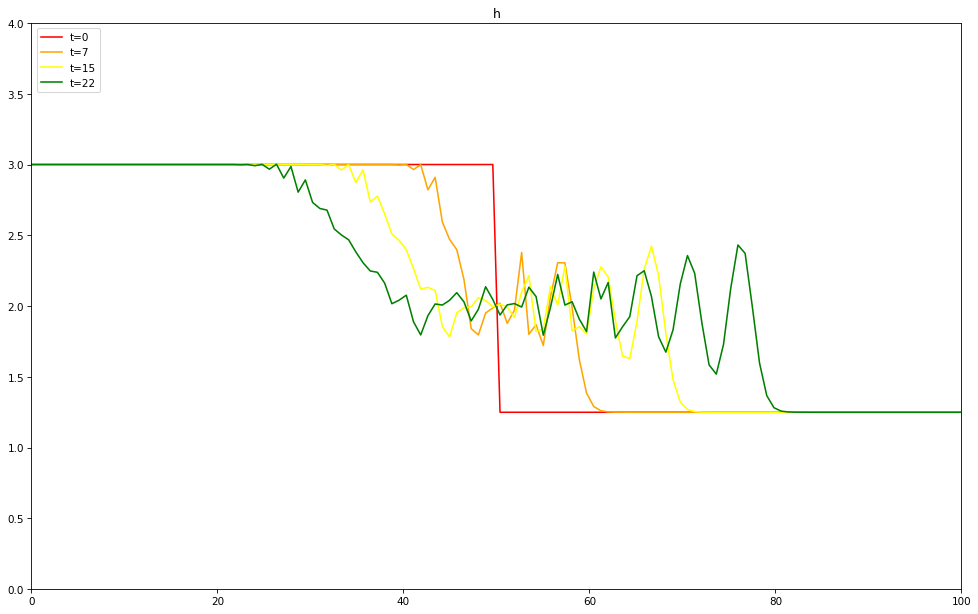
\includegraphics[scale = .7]{MauvaisSchema.png}
\end{figure}

Les oscillations de la hauteur d'eau h sont amplifiées au cours du temps.

\subsubsection{Flux de Lax-Friedrichs}

Essayons maintenant avec un terme supplémentaire :

$$ \mathcal{F}_{i+1/2} = \frac{F(U_i) + F(U_{i+1})}{2} - \alpha \frac{U_{i+1} - U_i}{2} \quad avec \quad \alpha = \frac{\Delta x}{\Delta t}$$

On a donc la formule suivante pour calculer $U_i ^{n+1}$:

$$ U_i ^{n+1} = U_i ^{n}  - \frac{\Delta t}{\Delta x} ( \frac{F(U_{i-1}) + F(U_{i+1})}{2} - \alpha \frac{U_i - U_{i-1}}{2} - \frac{F(U_{i+1}) + F(U_i)}{2} + \alpha \frac{U_{i+1} - U_i}{2} ) $$

En simplifiant, car $ \alpha \frac{\Delta t}{\Delta x} = 1 $, on trouve que :

$$ U_i ^{n+1} = \frac{U_{i+1} ^{n} + U_{i-1} ^{n}}{2}  - \frac{\Delta t}{2 \Delta x} ( F(U_{i+1} ^n ) - F(U_{i-1} ^n ) $$

On verra dans la section suivante que l'on peut choisir $\alpha$ plus finement et ayant les bonnes propriétés en fonction des valeurs propres du système étudié.

\subsubsection{Flux de Rusanov}

Revenons tout d'abord aux critères de choix d'un flux numérique. Deux conditions sont importantes : la consistance et la stabilité.

\textbf{Définition :} On dit que le schéma est consistant avec le système étudié si :

$$ f(U,U) = U \quad \forall U $$ 

\textbf{Définition :} On dit que le schéma est stable s'il préserve un domaine convexe invariant noté C, autrement dit, que les erreurs ne soient pas amplifiées :

$$ U_i ^n \in C \Rightarrow U_i ^{n+1} \in C  $$

En choisissant une valeur d'$\alpha$ bien posée dans le flux de Lax-Friedrichs, on obtient le flux de Rusanov :

$$ \mathcal{F}_{i+1/2} = \frac{F(U_i) + F(U_{i+1})}{2} - \alpha \frac{U_{i+1} - U_i}{2} $$

avec $ \alpha = \underset{U = U_i , U_{i+1}}{\sup} \underset{j = 1 , 2}{\sup} | \lambda_j(U) | $

Ce flux numérique vérifie bien les conditions de consistance et de stabilité.


\subsection{Validation de l'implémentation avec des tests}

Dans cette partie, nous allons effectuer des tests de notre implémentation (dont le code est en annexe).
Dans un premier temps, nous allons comparer nos résultats à des tests trouvés dans des ouvrages de référence.
Dans un second temps, nous allons observer numériquement la convergence des solutions calculées.

\subsubsection{Quelques exemples}

\paragraph{Le test du lac} \

Voyons d'abord un premier test trivial : en prenant une hauteur d'eau plate et un débit initial identiquement égal à zéro, on s'attend à ce que l'eau reste plate au cours du temps.
On vérifie 	alors avec les plots de la figure... que le schéma fonctionne bien sur cet exemple.

\begin{figure}
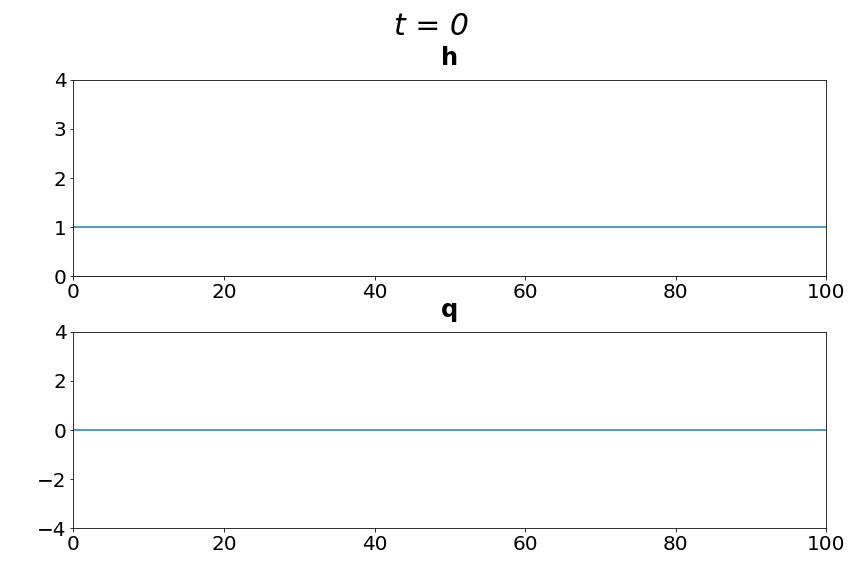
\includegraphics[scale = .6]{plat0}
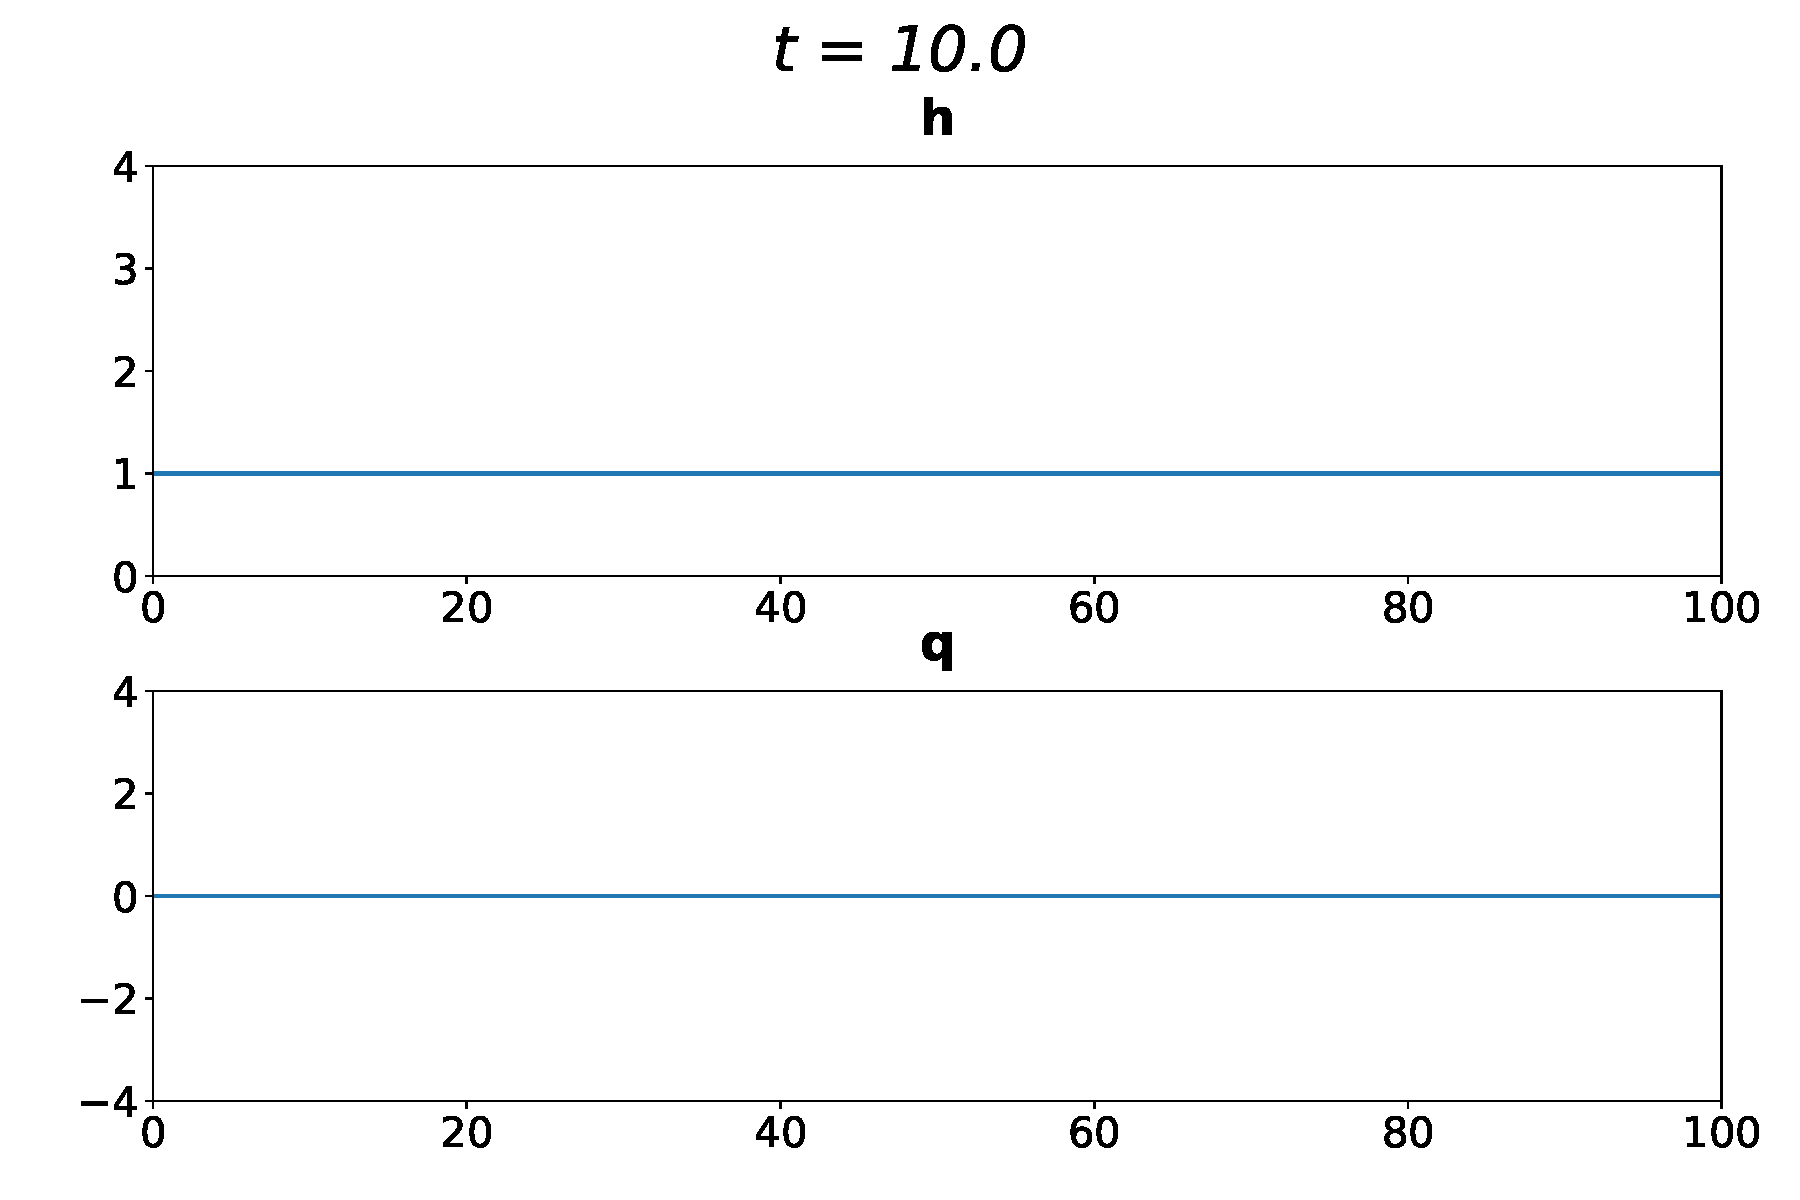
\includegraphics[scale = .6]{plat10} 
\caption{Un premier test : évolution d'une hauteur d'eau plate}
\end{figure}

\paragraph{Le test de la goutte d'eau} \

Partons maintenant de la condition initiale suivante : une bosse d'eau au milieu du domaine sans débit initial.

\begin{figure}
\centering
\includegraphics[scale = .7]{"bosse0"}
\end{figure}

Intuitivement, on s'attend à ce que la \og goutte \fg{} tombe et forme deux vagues qui partent vers chacun des deux bords du domaine.
C'est aussi ce que nous dit la référence \cite{RL} à la page 257. Et effectivement, voici ce que l'on observe (après environ 3 secondes et 8 secondes) :

\begin{figure}
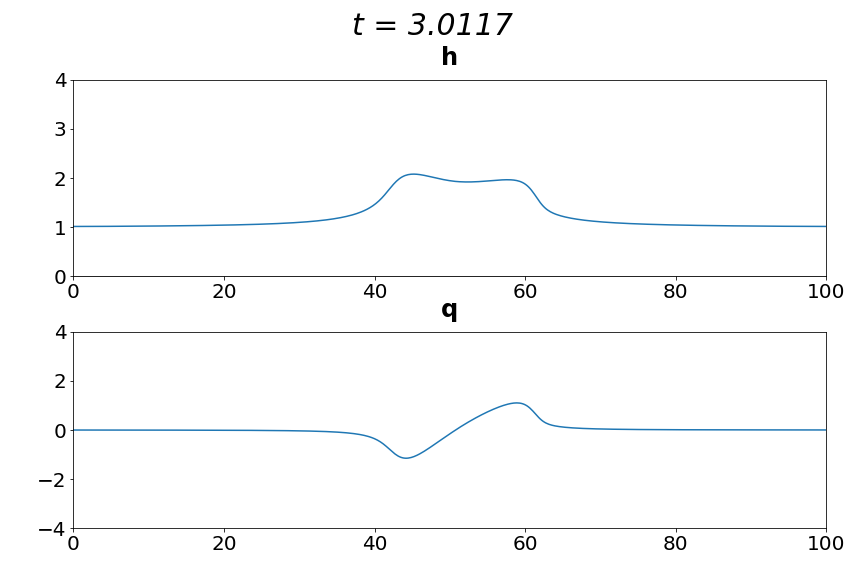
\includegraphics[scale = .6]{bosse4.png}
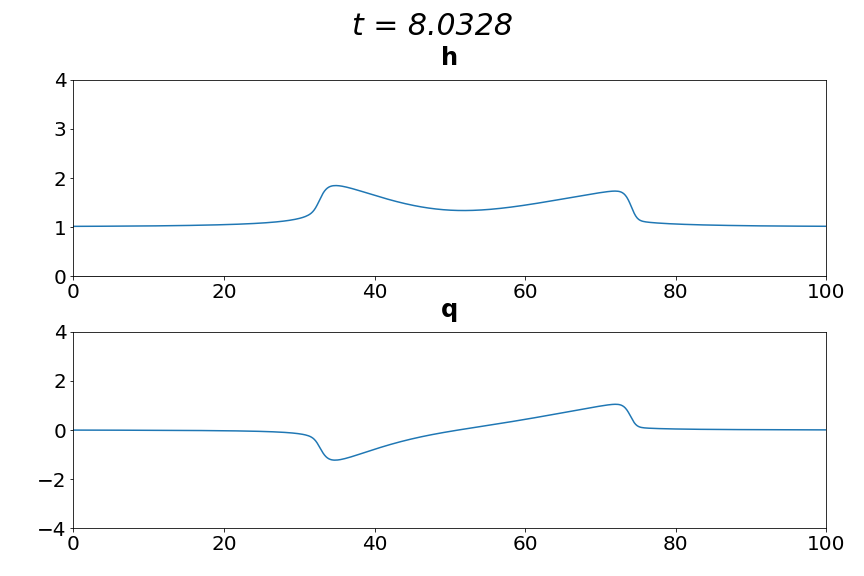
\includegraphics[scale = .6]{bosse10.png} 
\caption{Un deuxième test : une goutte d'eau}
\end{figure}

\paragraph{Le test de la rupture de barrage} \

Regardons maintenant un dernier test classique dans la littérature : la rupture de barrage.

\begin{figure}
\centering
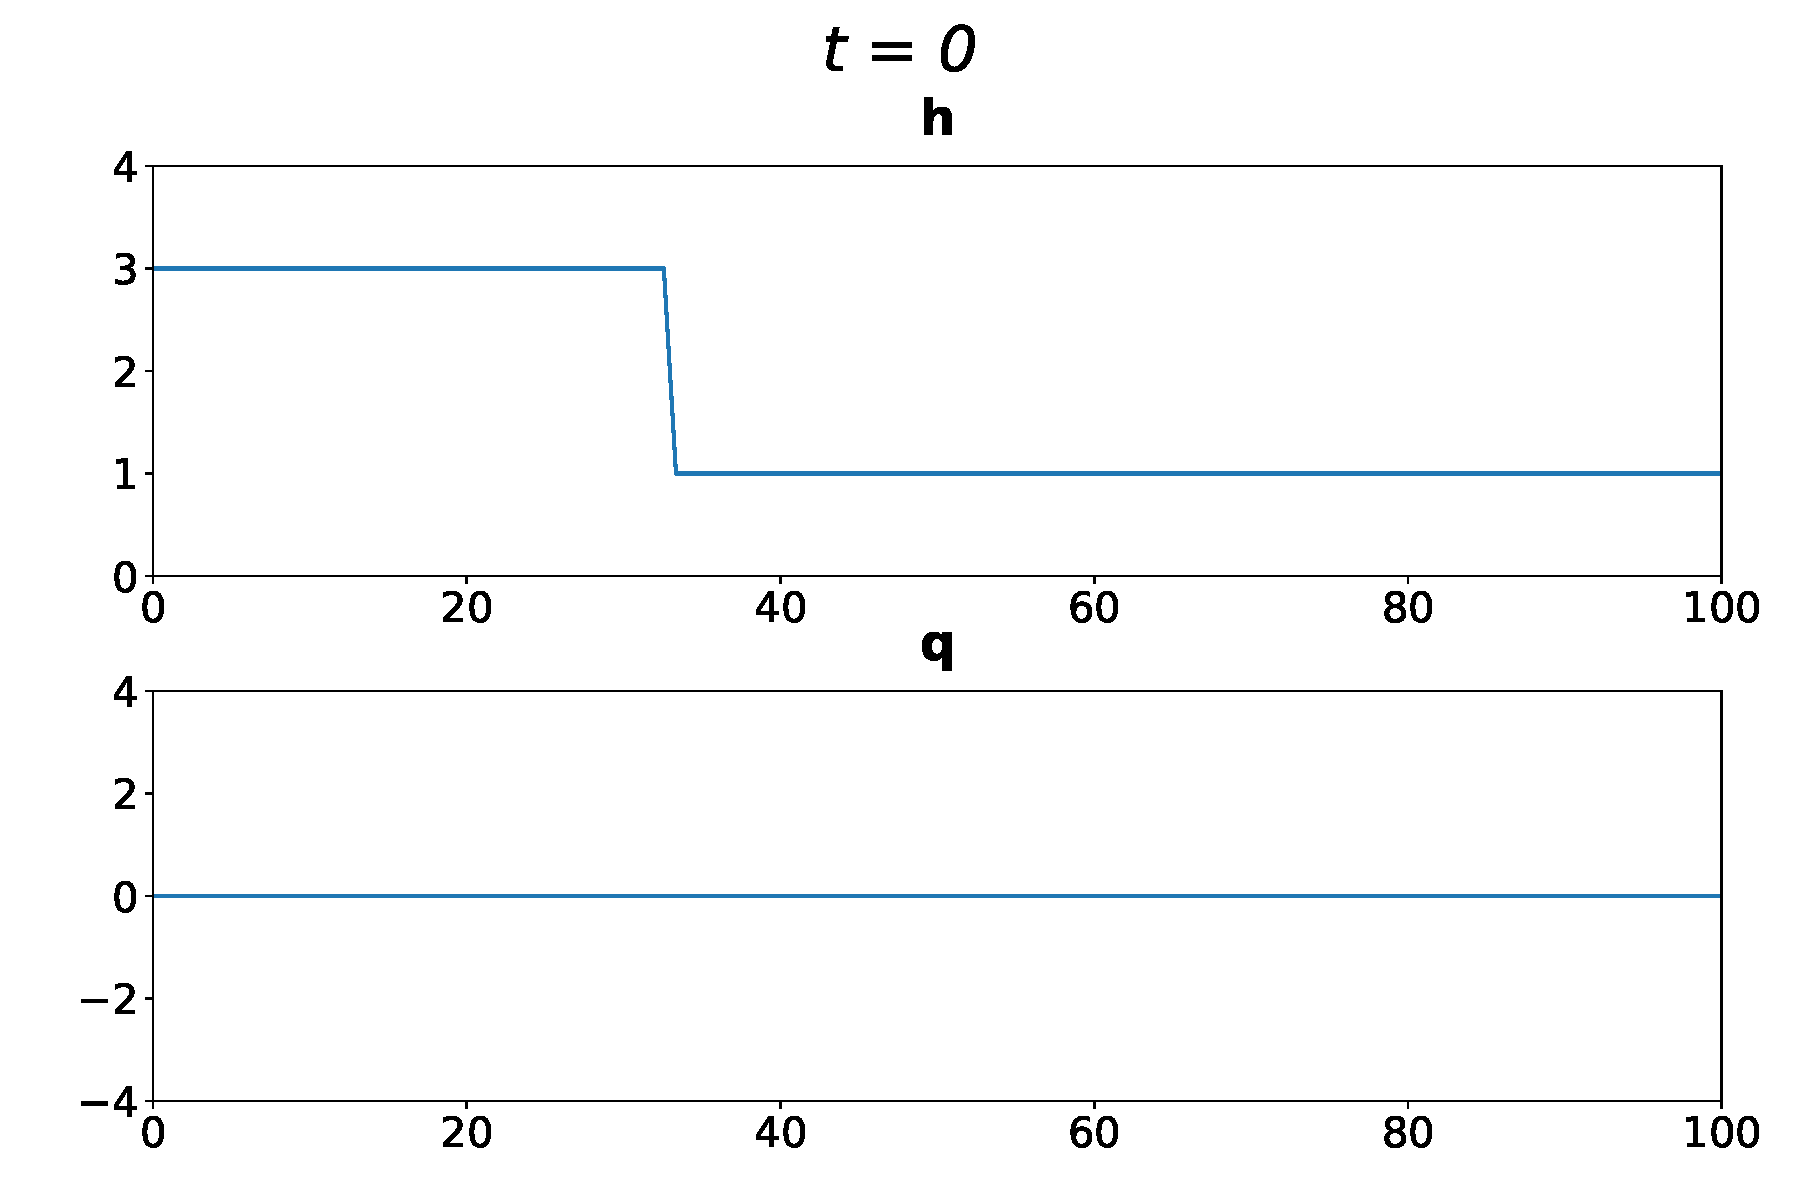
\includegraphics[scale = .7]{barrage0}
\end{figure}

L'eau forme une courbe en escalier (d'une seule marche) comme si elle était contenue dans une digue. On observe son évolution comme si la digue disparaissait juste après l'instant initial ; d'où le nom de
rupture de barrage. On observe le résultat suivant :

\begin{figure}
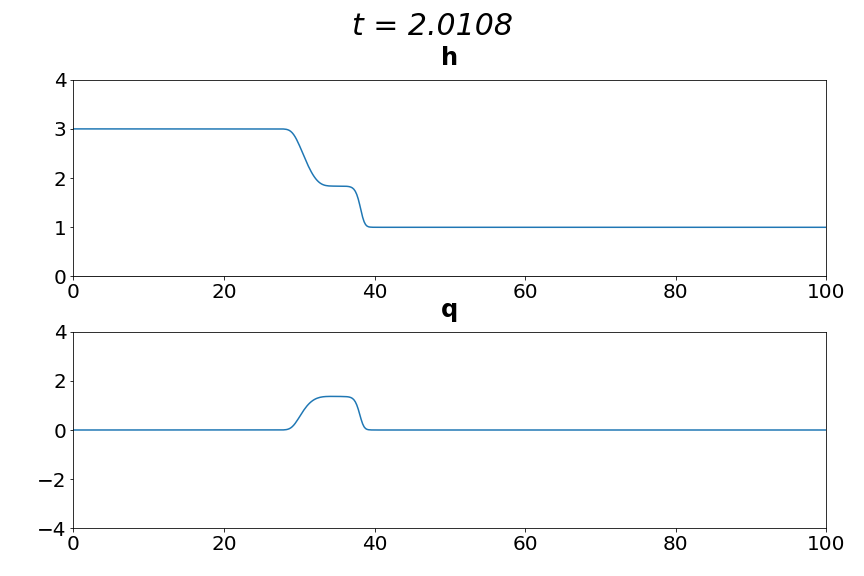
\includegraphics[scale = .6]{barrage1}
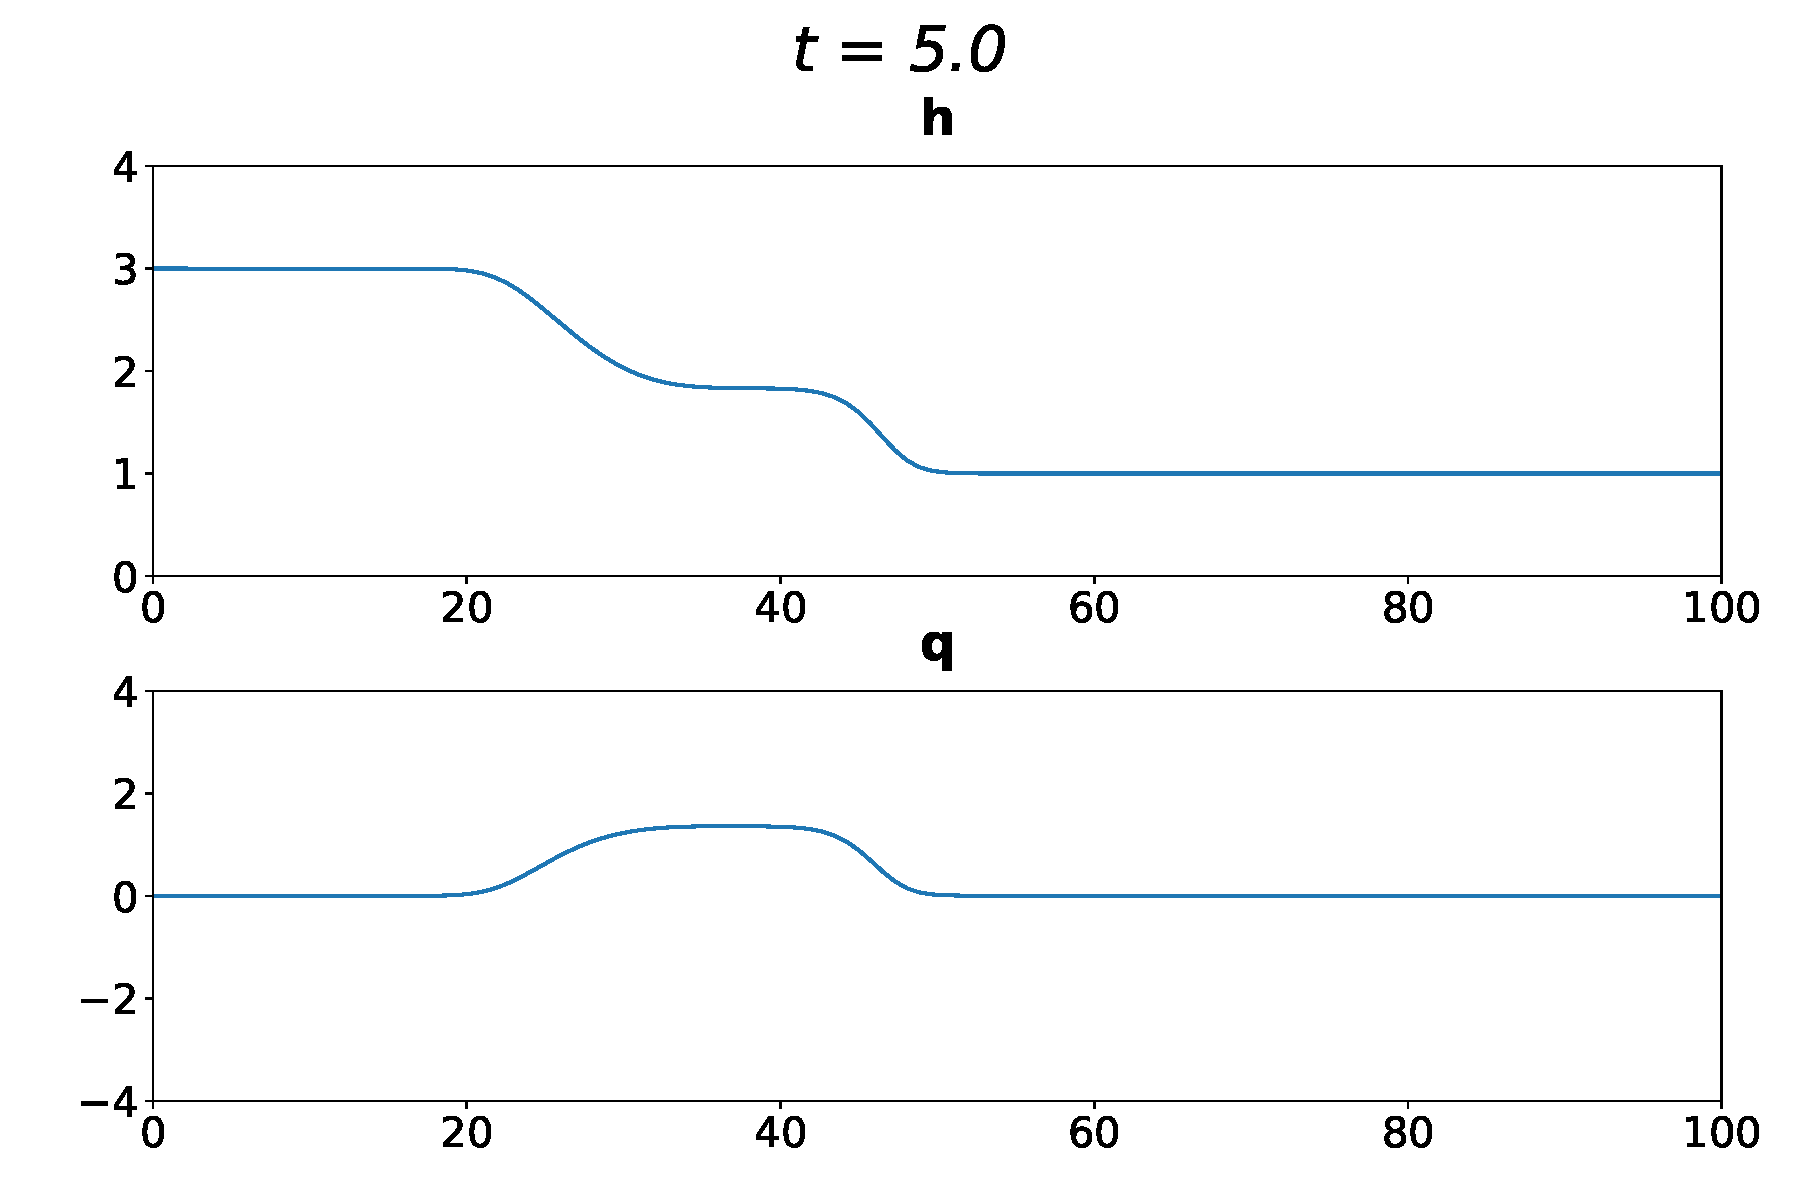
\includegraphics[scale = .6]{barrage5} 
\caption{Un deuxième test : une goutte d'eau}
\end{figure}

Ce résultat est conforme à ce que l'on observe dans \cite{RL} page 259. La dynamique des solutions obtenues par notre implémentation est donc la bonne sur ces quelques tests.

\subsubsection{Influence du pas spatial}

Nous allons faire une étude de convergence de type Cauchy : si la suite des approximations converge vers une limite, alors l'écart entre deux approximations numériques peut être rendu aussi petit qu'on le souhaite, pourvu que les paramètres de grilles soient assez grands (ou petits selon que l'on considère le nombre de points ou le pas).

Puisque le schéma de Rusanov est convergeant, on peut considérer que la solution calculée est la solution exacte (ou du moins est très proche de la solution exacte) lorsque le pas d'espace est très petit. Notons $U_{ex}$ cette solution que l'on considère exacte et $U_N$ la solution obtenue lorsque le nombre de points (strictement à l'intérieur du domaine) est $N$. On peut alors procéder comme il est courant de le faire au calcul de numérique de l'ordre du schéma, en effectuant le plot de $max_{x_i}|U_{ex}(x_i)-U_N(x_i)|$ ou de la norme $L^{2}$ discrète de $U_{ex}-U_N$ en fonction de $N$ ; les $x_i$ étant les points de la discrétisation.

Pour faire cette étude, on prend arbitrairement $\textbf{xMin}=0$, $\textbf{xMax}=1$  pour les bords du domaine et $\textbf{Tmax}=0,03$ pour le temps final de la simulation. Pour les conditions initiales on prend $h_{0}(x) = 2+\cos(5x)/2$ et $q_{0}\equiv 1$ pour la hauteur d'eau et le débit à l'instant initial. La topographie est prise constante égale à 0 ($Z\equiv 0$).

La convergence s'observe d'abord visuellement, en faisant le plot des solutions calculées pour des valeurs de $N$ de plus en plus grandes. On peut par exemple représenter graphiquement la hauteur d'eau de la solution $U_{ex}$ avec celle de  $U_N$. Dans la suite $h_{ex}$ et $h_{N}$ désigneront ces quantités. Les figures ci-dessous ont été obtenues avec $N=2^{k}$, $k$ allant de $3$ à $9$.

\begin{figure}
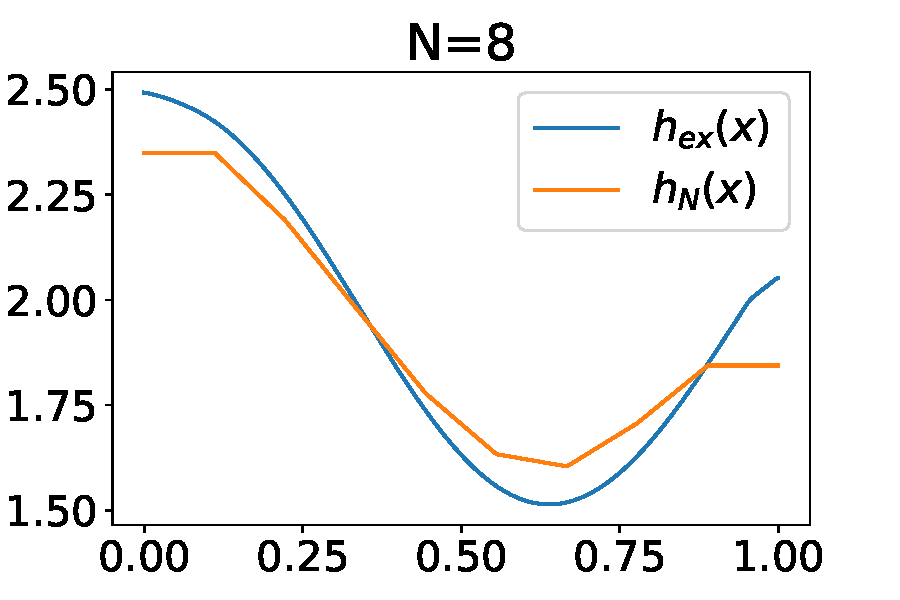
\includegraphics[scale = .6]{testconv8}
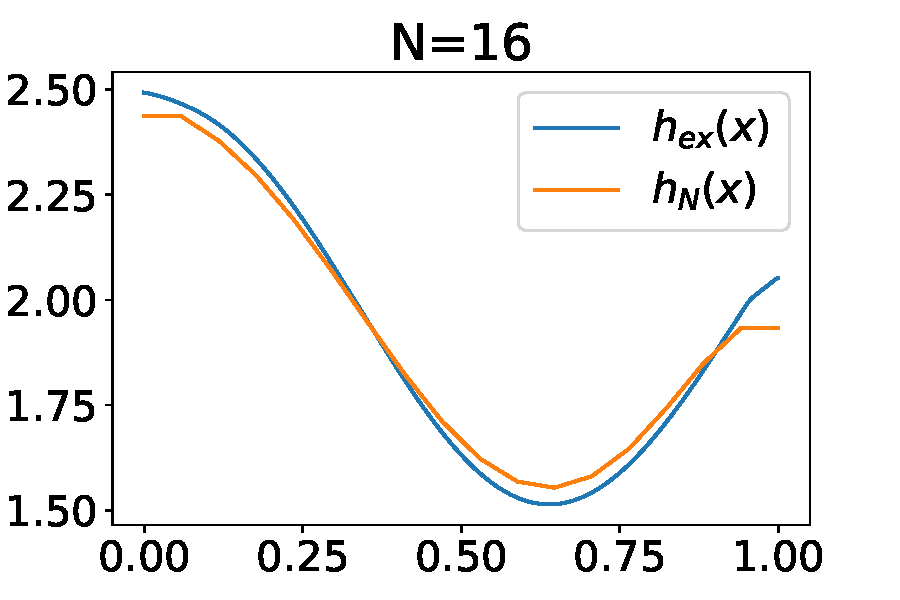
\includegraphics[scale = .6]{testconv16} 
\end{figure}

\begin{figure}
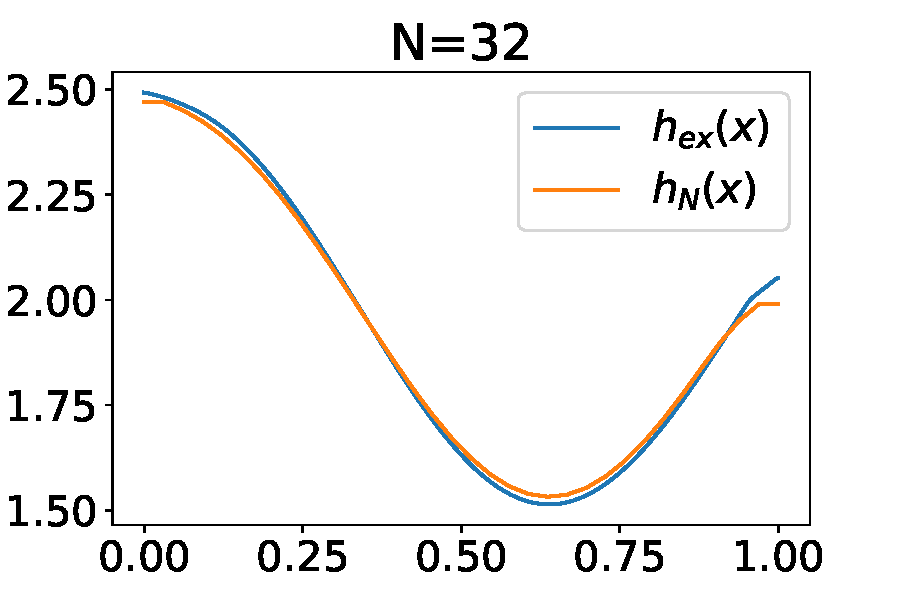
\includegraphics[scale = .6]{testconv32}
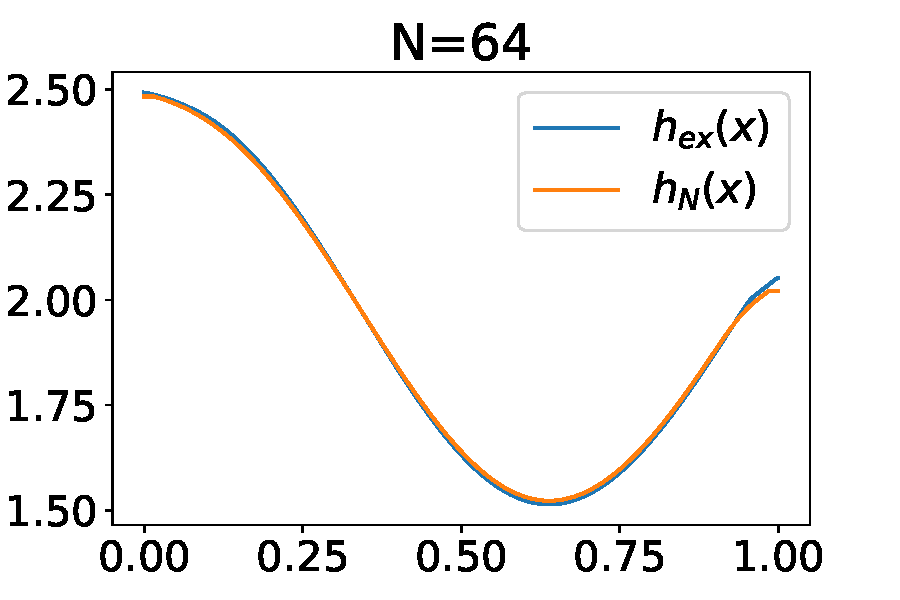
\includegraphics[scale = .6]{testconv64} 
\end{figure}

\begin{figure}
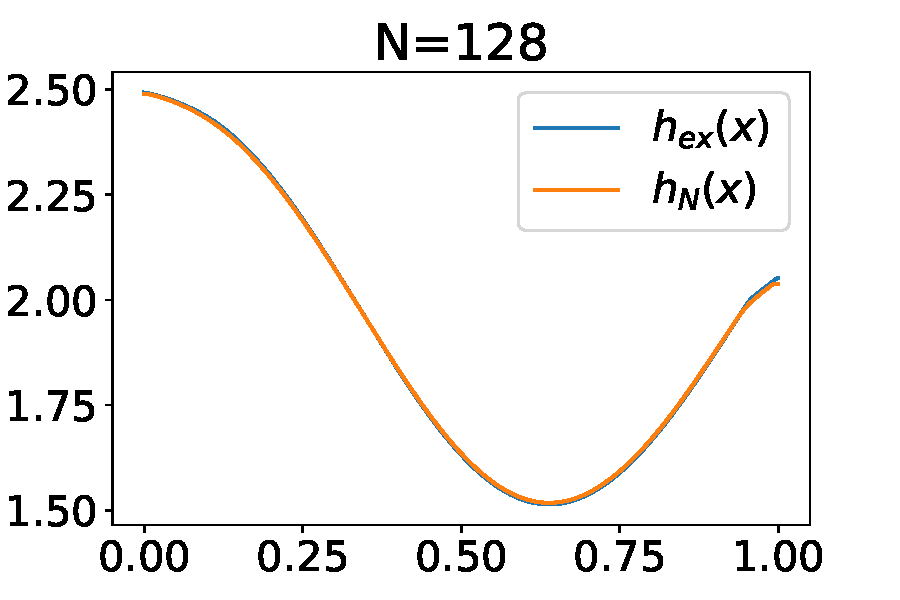
\includegraphics[scale = .6]{testconv128}
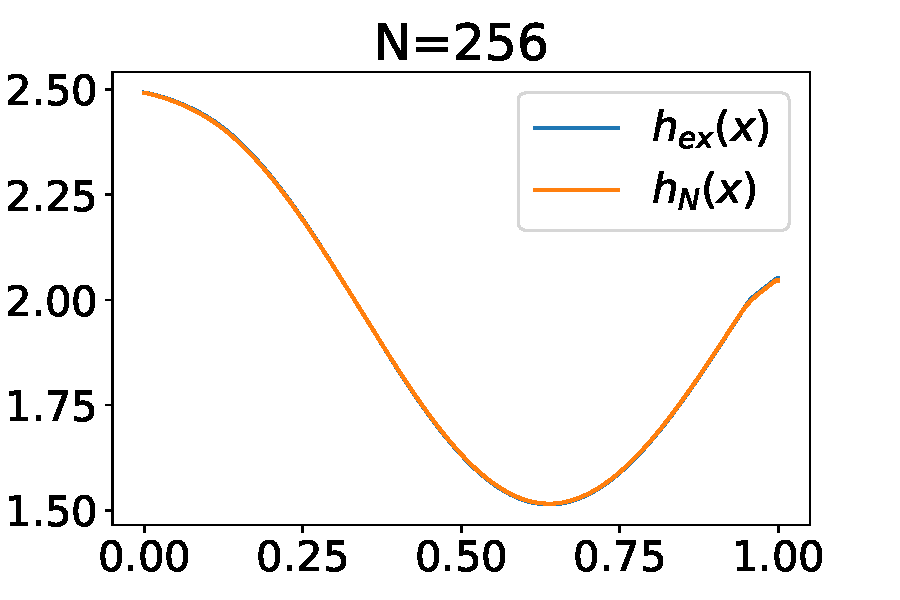
\includegraphics[scale = .6]{testconv256} 
\end{figure}


Regardons maintenant le plot du maximum de l'erreur entre $h_{ex}$ et $h_{N}$. Pour ce faire, on retient les points $x_{i}$ communs aux deux maillages.
Si la solution $U_{ex}$ correspond à une discrétisation de $N=2^{l}$ point intérieurs (comme c'est le cas dans notre implémentation), alors le maillage correspondant contiendra tous les maillages de $N=2^{k}$  point intérieurs avec $k\leq l$. Ainsi, les points $x_{i}$ communs aux deux maillages sont ceux du maillage pour $U_{N}$. Dès lors, on calcule facilement $max_{x_i}|U_{ex}(x_i)-U_N(x_i)|$. Voici les représentations obtenues avec cette manière de calculer l'erreur :

\begin{figure}
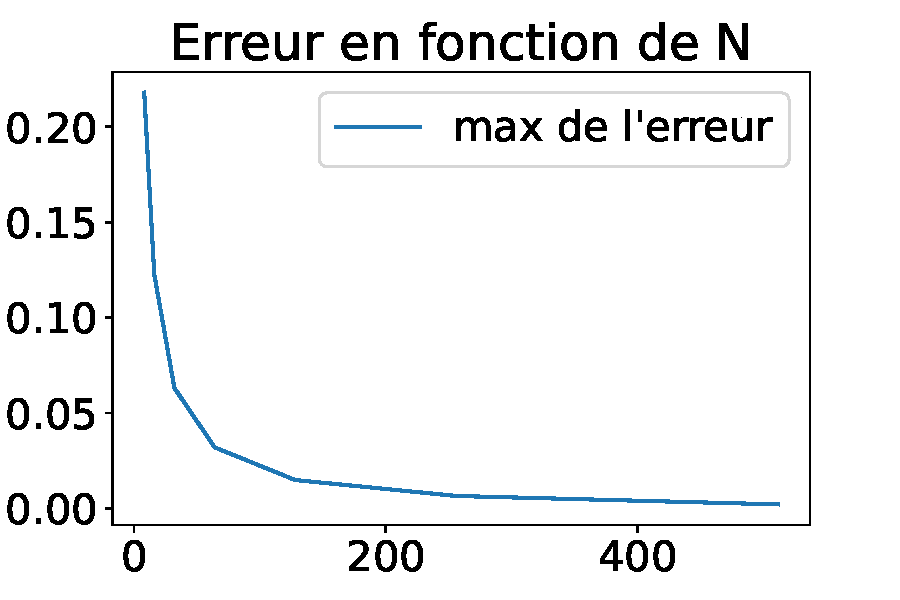
\includegraphics[scale = .6]{erreur}
\includegraphics[scale = .6]{erreurloglog} 
\end{figure}

Voyons maintenant l'erreur en norme $L^{2}$ discrète. Avant \c ca, définissons cette notion. La norme $L^{2}(a,b)$ d'une fonction $u$ de carré intégrable est donnée par $$\| u \|_{L^{2}(a,b)}=(\int_{a}^{b}u^{2}(x)~dx)^{\frac{1}{2}}.$$
Si $x_{0}=a<x_{1}<...<x_{N}=b$ discrétise $[a,b]$, alors par la relation de Chasles, on a $$\int_{a}^{b}u^{2}(x)~dx=\sum_{i=0}^{N-1}\int_{x_{i}}^{x_{i+1}}u^{2}(x)~dx\approx\sum_{i=0}^{N}u^{2}(x_{i})(x_{i+1}-x_{i}).$$
On a alors un analogue discret de la norme $L^{2}$ habituelle donné dans la définition qui suit.

\medskip

\begin{definition} Soit $N\in\mathbb{N}$ et $x_{0}=a<x_{1}<...<x_{N+1}=b$ la discrétisation uniforme de $[a,b]$ composée de $N+2$ points (N à l'intérieur et 2 aux bords). Posons $h=\frac{b-a}{N+1}$ le pas du maillage.
Soit $U=(u_{i})_{0\leq i \leq N+1}$ une approximation de la solution aux points du maillage. On définit la norme $L^{2}$ discrète de $U$ par $\| U \|_{L^{2}}=(h\sum_{i=0}^{N+1}u_{i}^{2})^{\frac{1}{2}}.$
\end{definition}

Voici les erreurs obtenues avec cette norme :

\begin{figure}
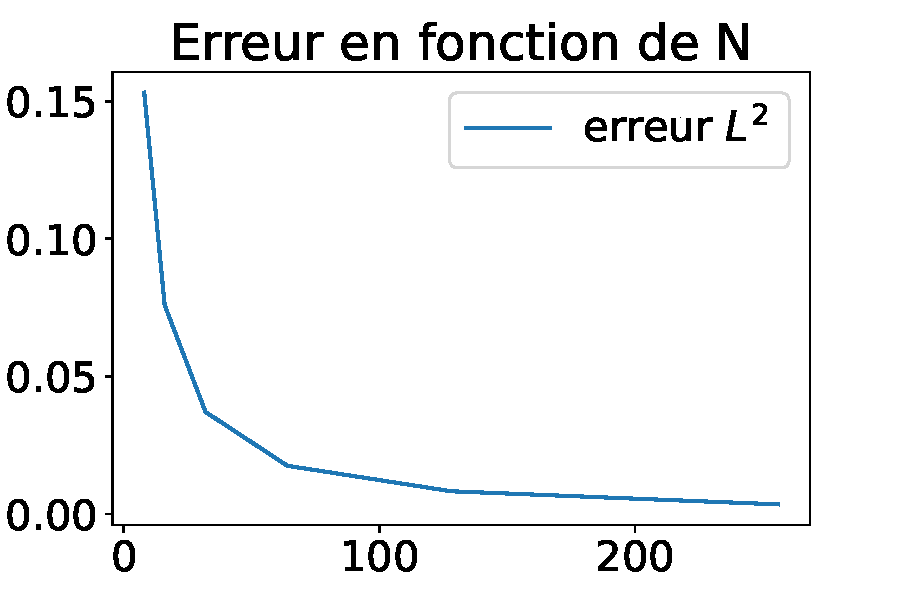
\includegraphics[scale = .6]{erreurL2}
\includegraphics[scale = .6]{erreurL2loglog} 
\end{figure}

En échelle loglog, on observe à chaque fois que l'erreur décroit selon une pente -1. Sur cet exemple, le schéma est donc d'ordre 1.

Des résultats similaires sont obtenus lorsque l'on affiche le débit $q$ plutôt que la hauteur d'eau $h$. De la même fa\c con, on peut faire varier les paramètres $\textbf{xMin}$, $\textbf{xMax}$, $\textbf{Tmax}$ ainsi que les conditions initiales et on arrive aux mêmes conclusions.

\subsubsection{Influence du pas temporel}

Dans ce paragraphe, nous allons faire une étude similaire à celle qui précède, sauf que cette fois nous allons fixer le nombre $N=2^{7}$ de points (intérieurs) de la discrétisation et faire varier le pas d'espace $\tau$.
Tous les autres paramètres restent inchangés et les conditions initiales sont encore les mêmes.

$\tau$ va être pris égal à $\frac{1}{2^{k}}$ avec $k$ variant de $8$ à $17$. On considère que l'on est très proche de la solution exacte lorsque $\tau = \frac{1}{2^{17}}$ et on note $U_{ex}$ la solution obtenue avec ce pas de temps.
On note $U_{\tau}$ une solution obtenue avec un pas plus grand (c'est à dire avec $k\leq17)$. En augmentant $k$, on s'attend à voir converger la solution $U_{\tau}$ vers $U_{ex}$. Nous allons le vérifier sur les hauteurs d'eau. Dans la suite, $h_{ex}$ désignera la hauteur d'eau de la solution $U_{ex}$ et $h_{\tau}$ celle de $U_{\tau}$.

\begin{figure}
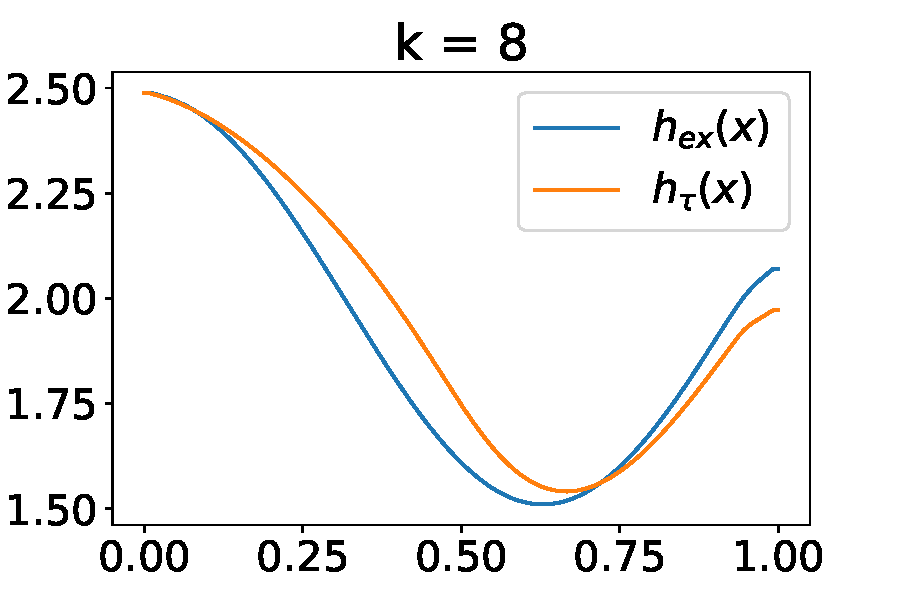
\includegraphics[scale = .6]{testconvtau8}
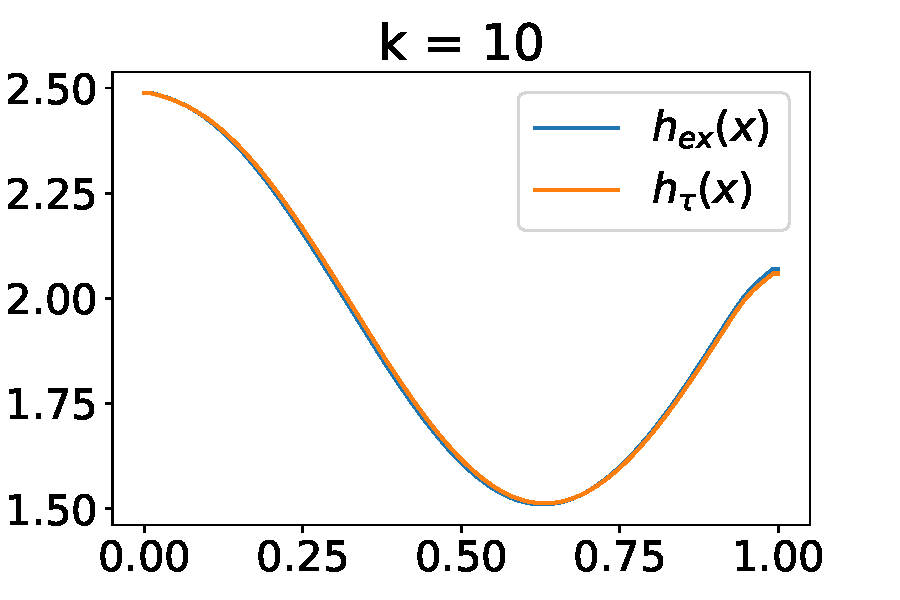
\includegraphics[scale = .6]{testconvtau10} 
\end{figure}

\begin{figure}
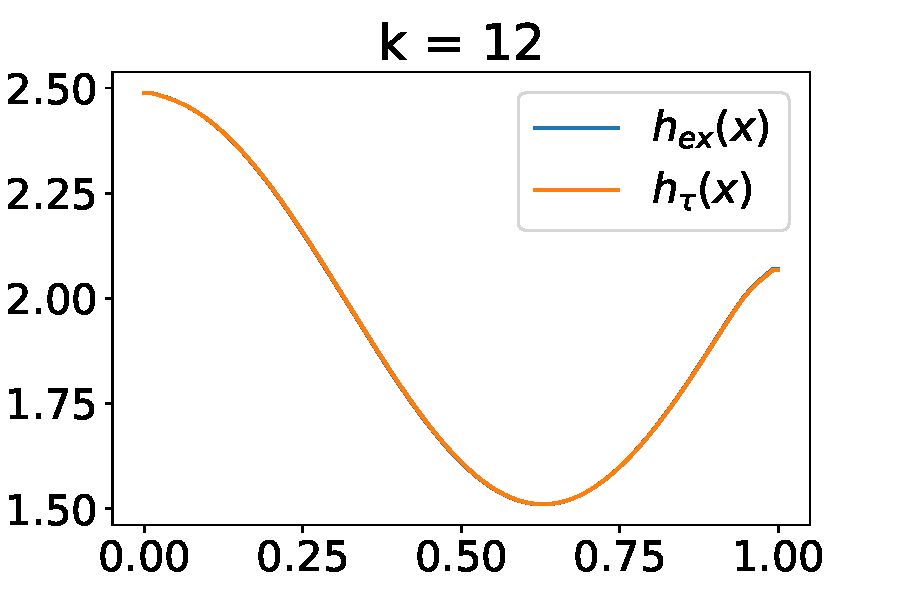
\includegraphics[scale = .6]{testconvtau12}
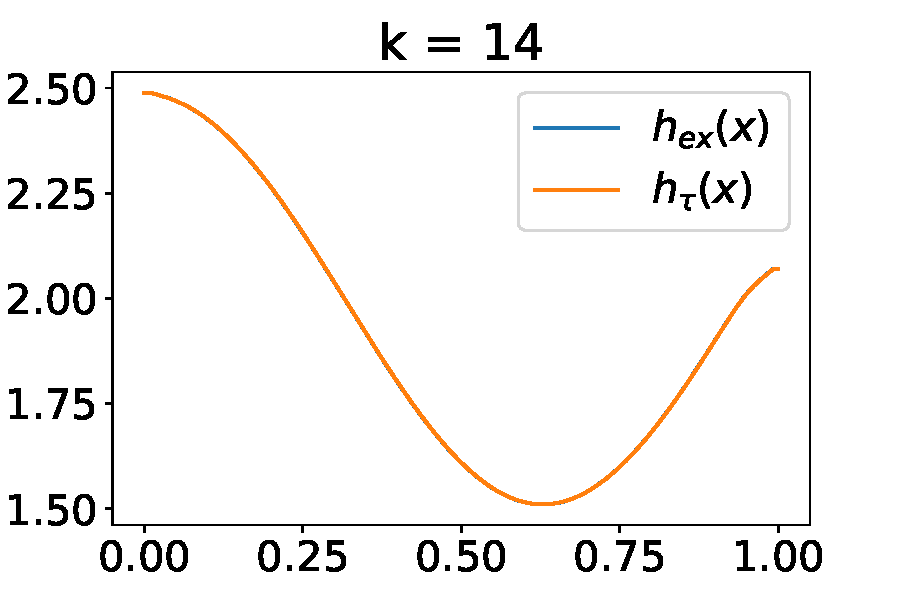
\includegraphics[scale = .6]{testconvtau14} 
\end{figure}

Effectivement, on observe bien la convergence des solutions approchées lorsque $k$ augmente. Nous allons quantifier cette convergence en effectuant la représentation graphique de l'erreur en norme $L^{2}$ discrète comme dans le paragraphe précédent.

\begin{figure}
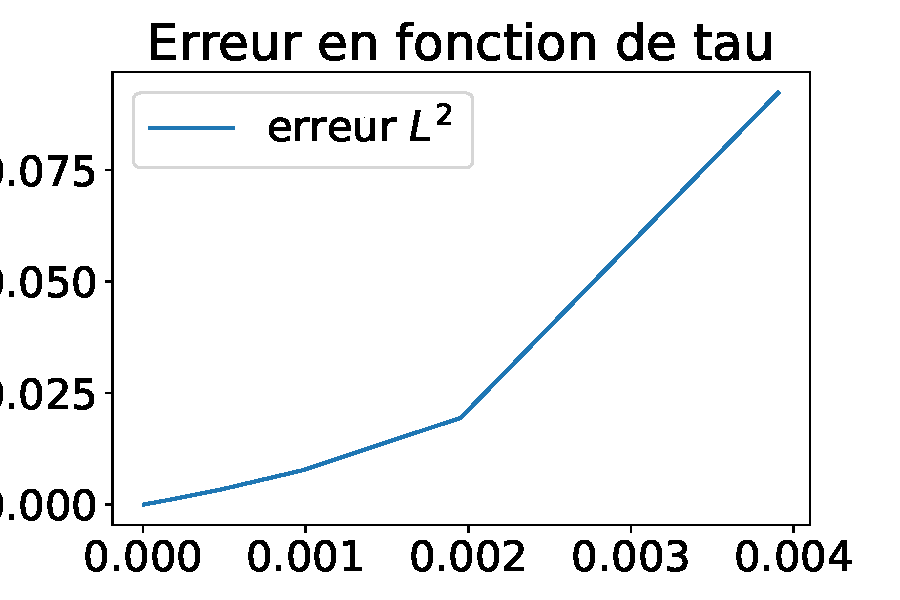
\includegraphics[scale = .6]{erreurtauL2}
\includegraphics[scale = .6]{erreurloglogtauL2} 
\end{figure}

On voit que plus $\tau$ est petit et moins l'erreur entre $h_{\tau}$ et $h_{ex}$ (en norme $L^{2}$) est importante. En échelle loglog, la courbe de l'erreur est approximativement une droite de pente égale à 1. Ainsi, le schéma est d'ordre 1 en temps sur cet exemple. Des résultats similaires sont obtenus lorsque l'on fait varier les paramètres $\textbf{xMin}$, $\textbf{xMax}$, $\textbf{Tmax}$ ainsi que les conditions initiales. 

Dans les simulations faites, les solutions calculées sont stables dans la mesure où le pas de temps $\tau$ a été pris suffisamment petit. Pour rappel, le schéma de Rusanov est stable sous la condition CFL locale suivante :

$$
\underset{j\in \{i,i+1\}}{\max} \underset{k\in\{1,2\}}{\max} |\lambda_{k}(U_{j}^{n}) | \tau^{n} \leq \frac{h}{2}.
$$

A chaque étape $n$ de la simulation, il faut donc prendre garde à ce que le nouveau pas de temps vérifie cette condition. Sinon, la stabilité n'est pas garantie. Par exemple, si l'on reprend le même contexte que l'étude qui précède mais que l'on choisit de prendre à chaque étape $n$ un pas de temps $$\tau^{n}=\frac{3}{2}~\frac{h}{2\times\underset{j\in \{i,i+1\}}{\max} \underset{k\in\{1,2\}}{\max} |\lambda_{k}(U_{j}^{n}) |},$$

la condition CFL n'est pas vérifiée et voici ce que l'on obtient pour la hauteur d'eau $h_{\tau^{n}}$ correspondante :

\begin{figure}
\centering
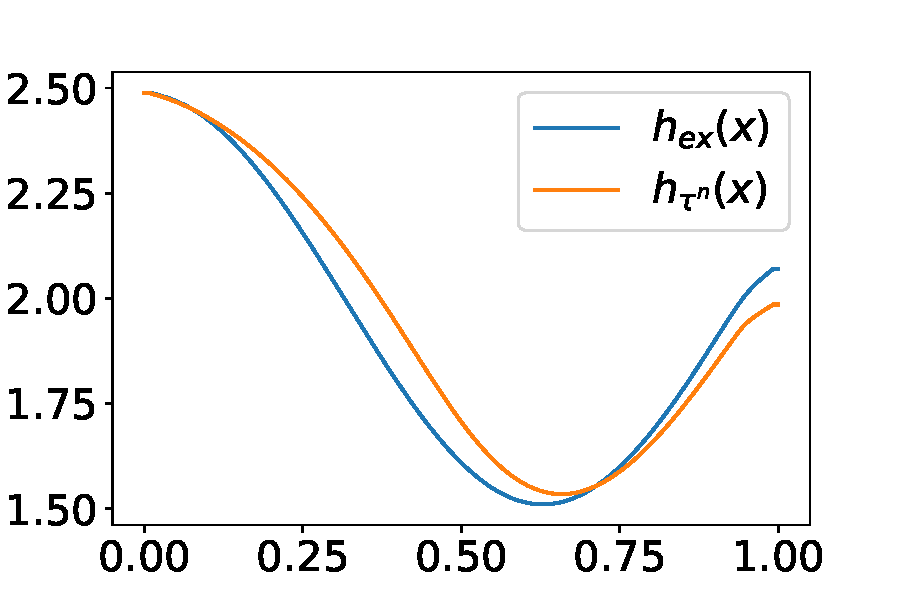
\includegraphics[scale = .8]{CFL1}
\end{figure}

Après un petit laps de temps, la solution approchée est déjà très éloignée de la solution exacte. Et en prenant un pas encore plus grand, par exemple $$\tau^{n}=1,9~\frac{h}{2\times\underset{j\in \{i,i+1\}}{\max} \underset{k\in\{1,2\}}{\max} |\lambda_{k}(U_{j}^{n}) |},$$ le phénomène empire encore :

\begin{figure}
\centering
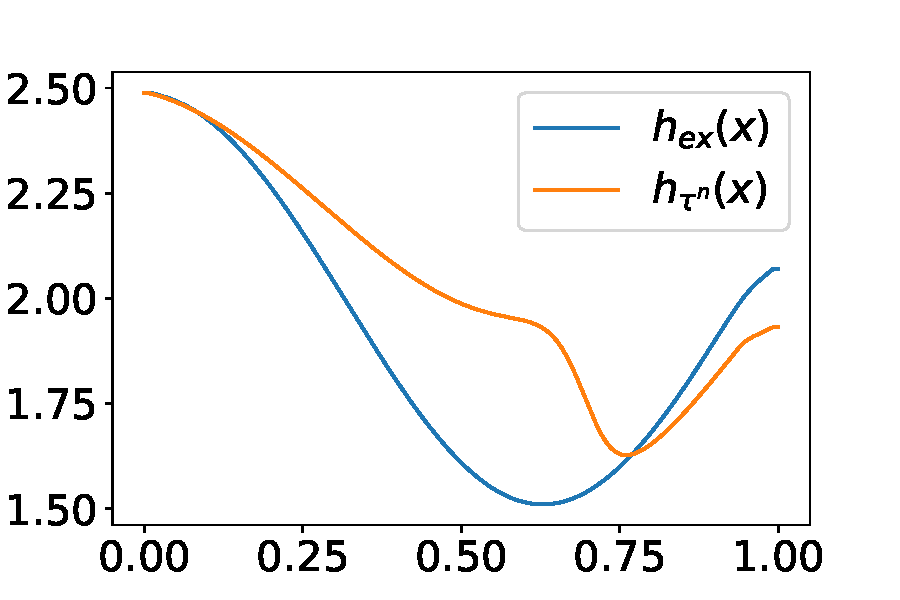
\includegraphics[scale = .8]{CFL2}
\end{figure}

Il faut donc veiller à ce que la condition CFL soit vérifiée, sans quoi le schéma propage des erreurs importantes.

\begin{comment}

Voici des représentations de la solution à différents instants (approximativement $t=0, 5, 10, 15$ et $20$ secondes) avec pas de temps égal $0.5\tau, \tau$ et $2\tau$ :

\begin{figure}[h]
\begin{center}$
\begin{array}{ccc}
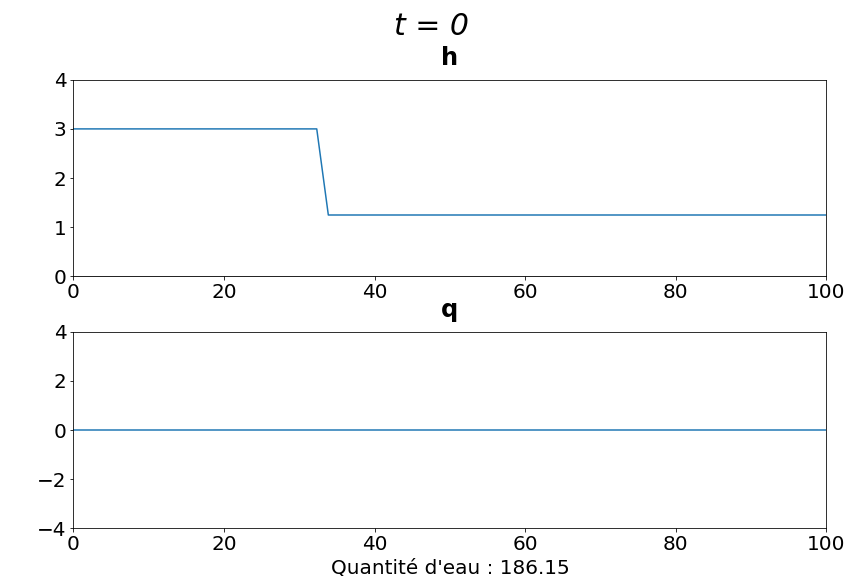
\includegraphics[scale = .35]{t0_tau05.png} &
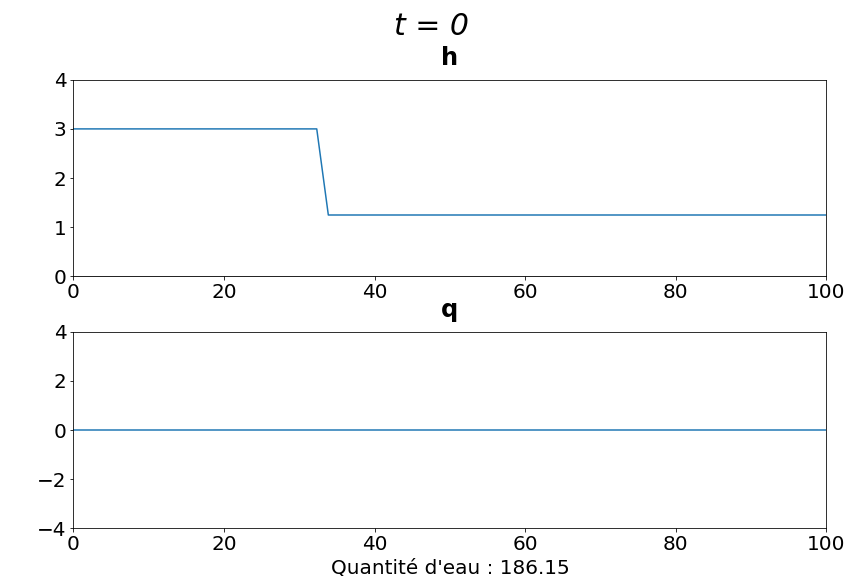
\includegraphics[scale = .35]{t0_tau.png} &
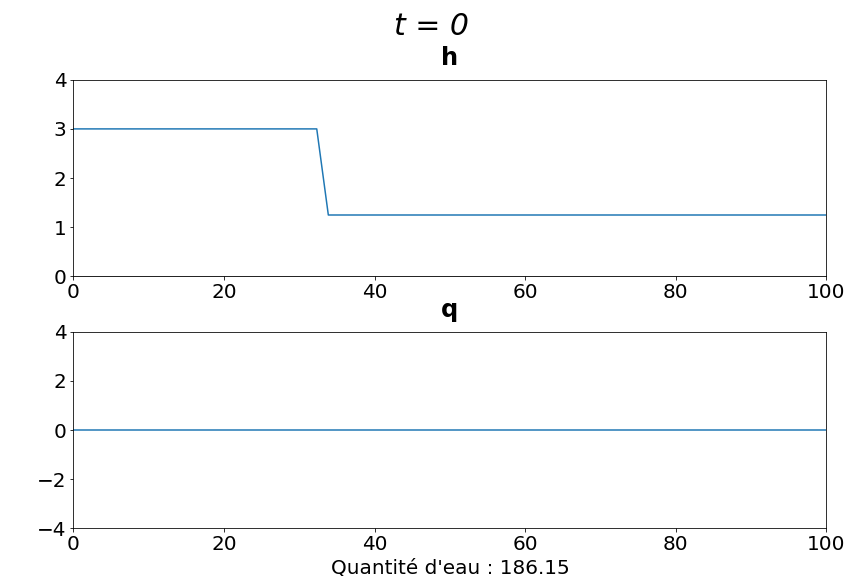
\includegraphics[scale = .35]{t0_tau2.png}
\\
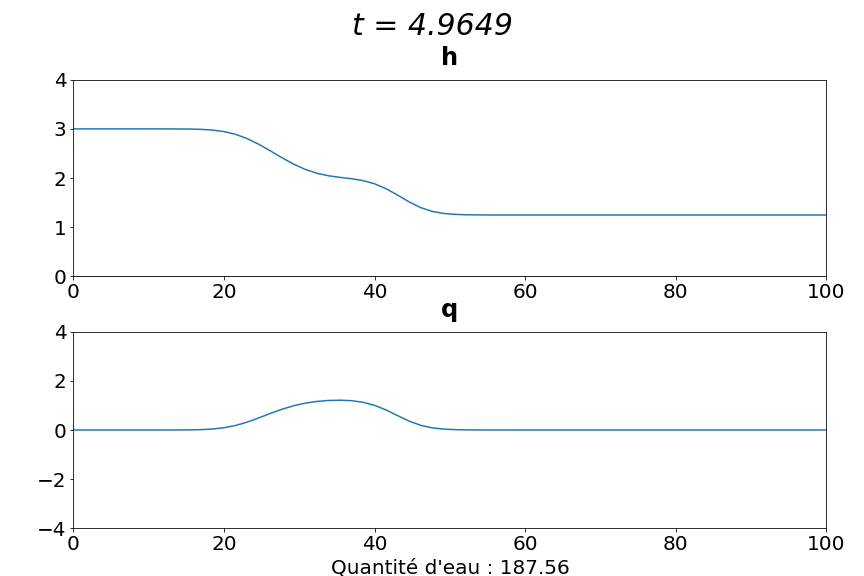
\includegraphics[scale = .35]{t5_tau05.png} &
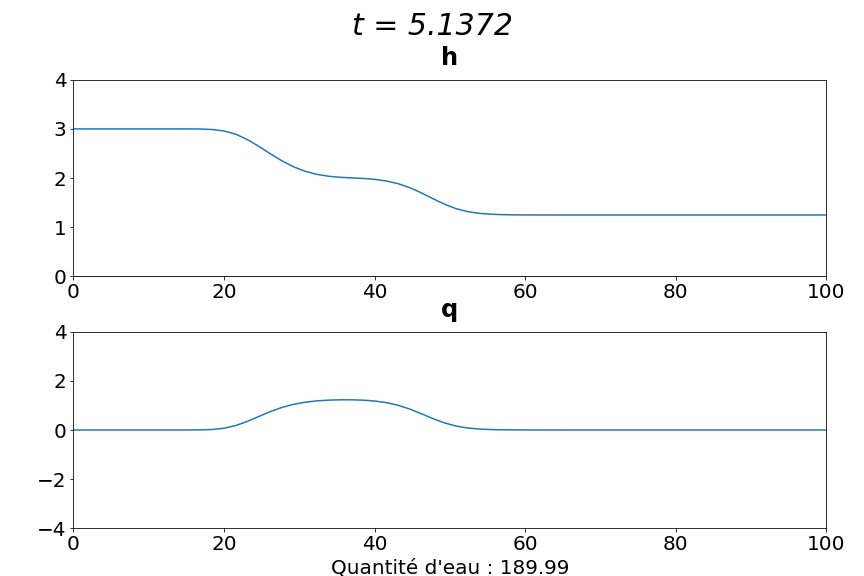
\includegraphics[scale = .35]{t5_tau.png} &
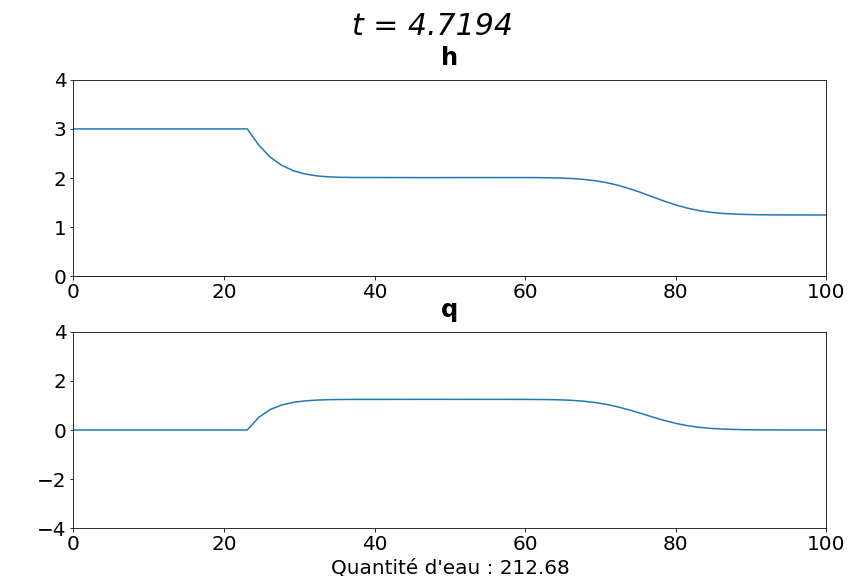
\includegraphics[scale = .35]{t5_tau2.png}
\\
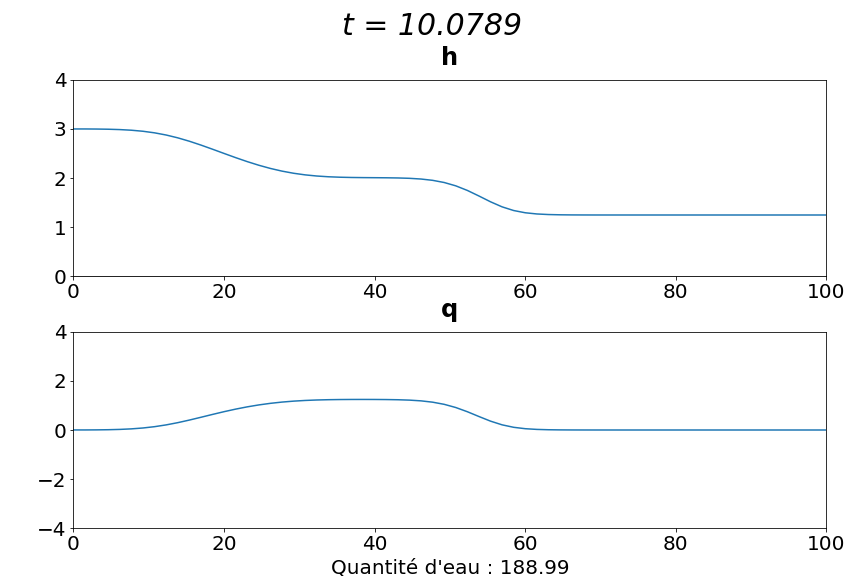
\includegraphics[scale = .35]{t10_tau05.png} &
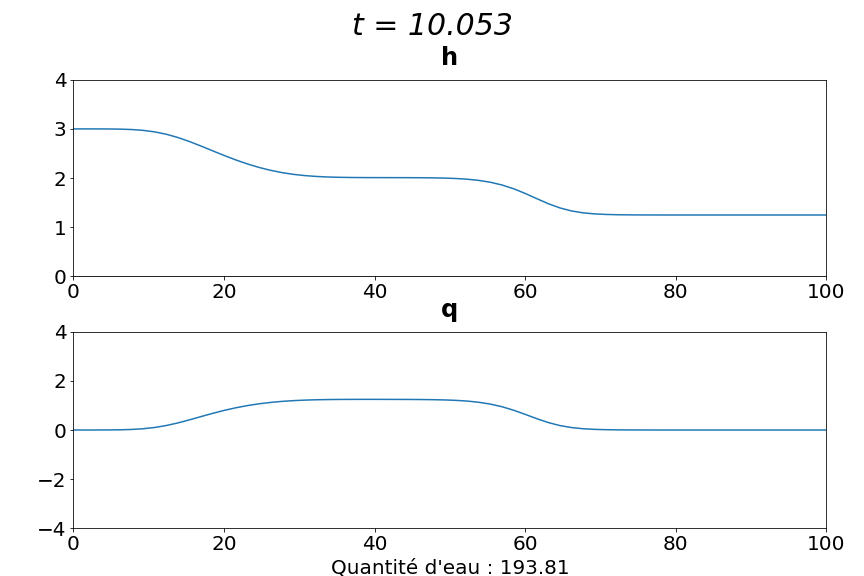
\includegraphics[scale = .35]{t10_tau.png} &
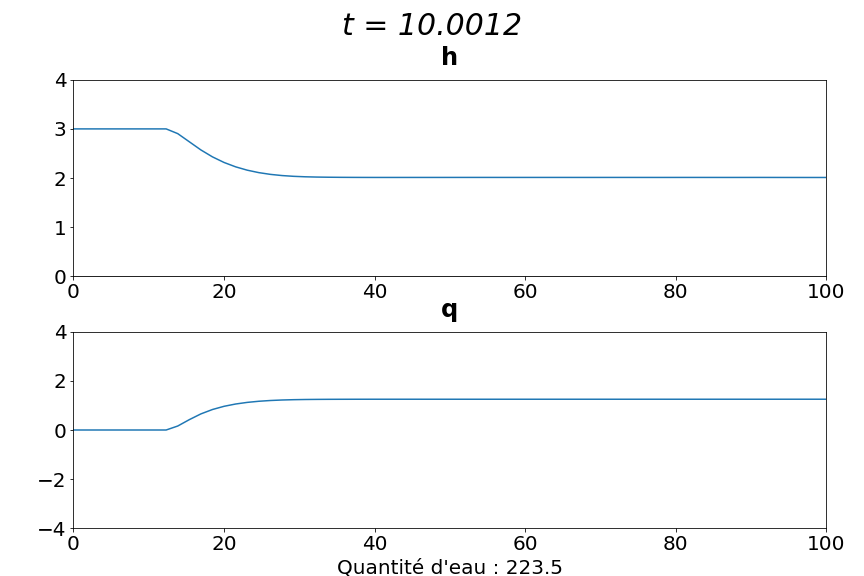
\includegraphics[scale = .35]{t10_tau2.png}
\\
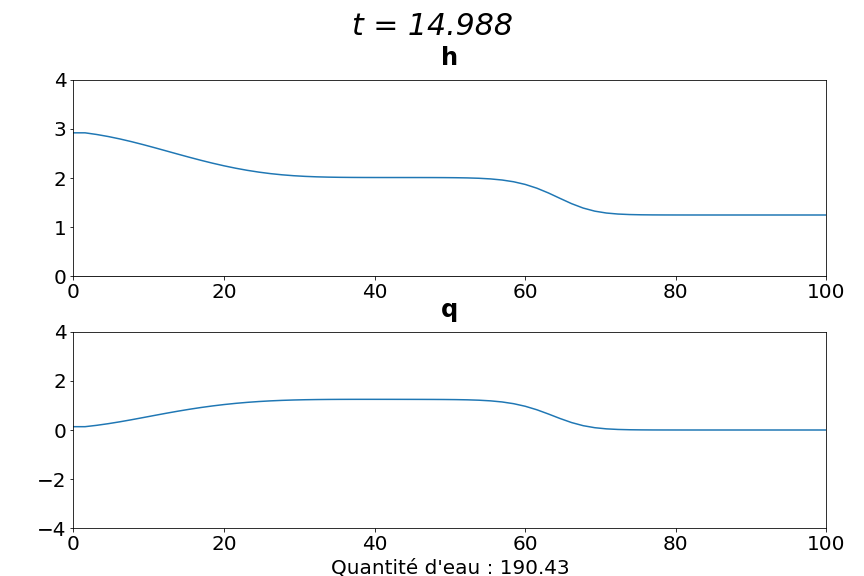
\includegraphics[scale = .35]{t15_tau05.png} &
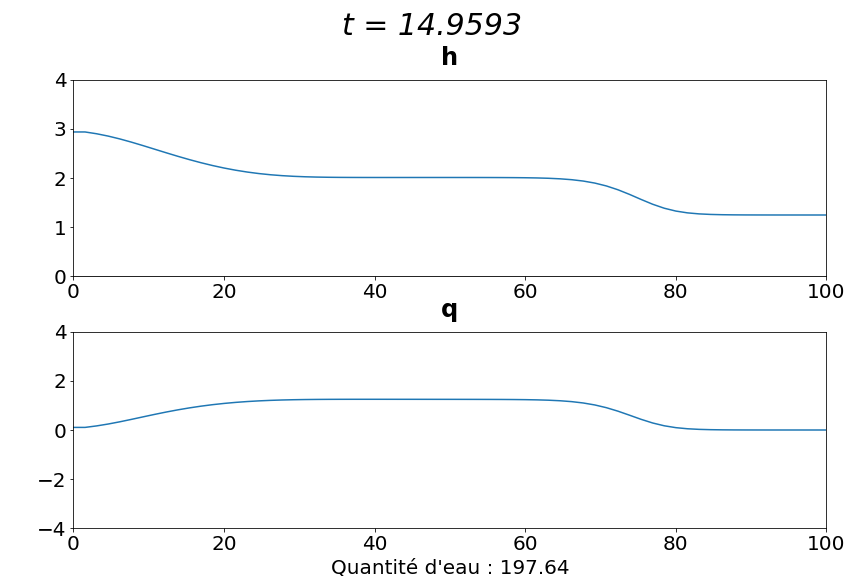
\includegraphics[scale = .35]{t15_tau.png} &
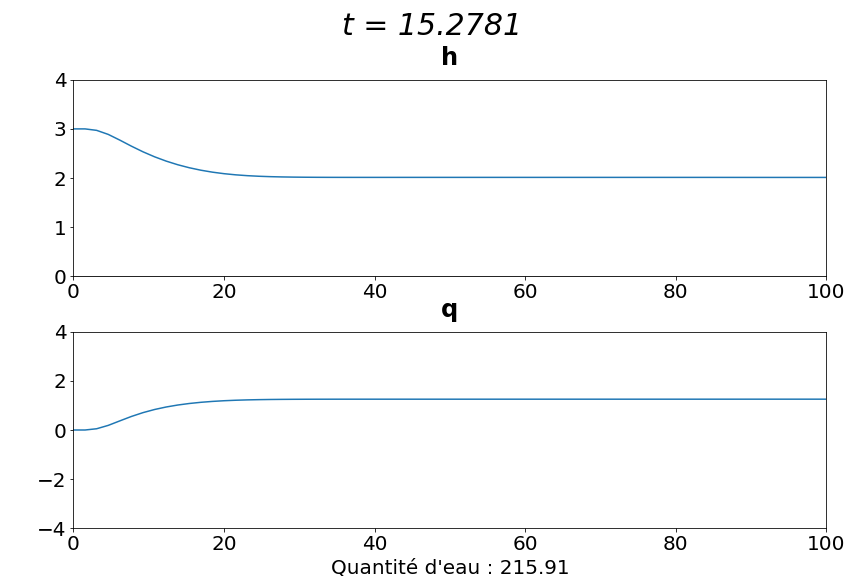
\includegraphics[scale = .35]{t15_tau2.png}
\end{array}$
\end{center}
\caption{Simulations pour différentes valeurs de $\tau$}
\end{figure}

On remarque immédiatement l'influence du pas temporel sur la conservation de la quantité d'eau. Plus le pas est choisi petit et meilleure est la conservation. On observe une dynamique similaire pour les deux cas qui respectent la condition CFL ($\tau$ et $0.5\tau$). Néanmoins, les évolutions sont quelque peu différentes (la vague issue de la rupture de barrage se déplace plus lentement lorsque le pas de temps est $0.5\tau$ ; cette différence dans les deux solutions obtenues vient peut être du fait que la condition doit être respectée strictement). Lorsque la condition CFL n'est pas vérifiée, l'évolution est très différente.


On retrouve le même phénomène dans le cas de la goutte d'eau qui tombe au centre du repère : voici les représentations pour $t=0, 10, 20, 30$ secondes, avec un pas de temps égal à $0.5\tau, \tau$ et $2\tau$.

\begin{figure}[h]
\begin{center}$
\begin{array}{ccc}
\includegraphics[scale = .35]{"deltaT=.5 tau t=0 N=64"} &
\includegraphics[scale = .35]{"deltaT=.5 tau t=0 N=64"} &
\includegraphics[scale = .35]{"deltaT=.5 tau t=0 N=64"}
\\
\includegraphics[scale = .35]{"deltaT=.5 tau t=10 N=64"} &
\includegraphics[scale = .35]{"deltaT=tau t=10 N=64"} &
\includegraphics[scale = .35]{"deltaT=2tau t=10 N=64"}
\\
\includegraphics[scale = .35]{"deltaT=.5 tau t=20 N=64"} &
\includegraphics[scale = .35]{"deltaT=tau t=20 N=64"} &
\includegraphics[scale = .35]{"deltaT=2tau t=20 N=64"}
\\
\includegraphics[scale = .35]{"deltaT=.5 tau t=30 N=64"} &
\includegraphics[scale = .35]{"deltaT=tau t=30 N=64"} &
\includegraphics[scale = .35]{"deltaT=2tau t=30 N=64"}
\end{array}$
\end{center}
\caption{Simulations pour différentes valeurs de $\tau$}
\end{figure}

De même, plus le pas temporel est faible, plus la quantité d'eau est conservée au cours du temps. On remarque aussi que la quantité d'eau est bien conservée quand la vague est au centre du repère. Cependant, quand elle atteint le bord et disparaît aux limites, la quantité d'eau baisse brutalement ( il suffit de comparer la quantité entre $t=0\ s$ et $t=20\ s$ puis la quantité entre $t=20\ s$ et $t=30\ s$ ). 
\end{comment}

\newpage
\section{Cas 2D}

\subsection{Présentation des équations}

Dans le cas bi-dimensionnel, nous avons maintenant trois inconnues : $h$, la hauteur de l'eau, ainsi que $u$ et $v$, la vitesse de l'eau selon l'axe $x$ et $y$ respectivement.

Nous avons les trois équations suivantes : 

$$\left\{
    \begin{array}{lll}
        \frac{\partial h}{\partial t} + \frac{\partial hu}{\partial x} + \frac{\partial hv}{\partial y} = 0 \\
        \frac{\partial hu}{\partial t} + \frac{\partial}{\partial x} ( hu^2 + \frac{gh^2}{2} ) + \frac{\partial}{\partial y} ( huv  ) = 0 \\
        \frac{\partial hv}{\partial t} + \frac{\partial}{\partial x} ( huv ) + \frac{\partial}{\partial y} ( hv^2 + \frac{gh^2}{2} ) = 0
    \end{array}
\right.
$$

En posant : 
$ W = \left[ {\begin{array}{c}   h \\    hu \\    hv \\  \end{array} } \right] $ ; 
$ F(W) = \left[ {\begin{array}{c}   hu \\    hu^2 + \frac{gh^2}{2}  \\    huv  \\  \end{array} } \right] $ ;
$ G(W) = \left[ {\begin{array}{c}   hv \\    huv  \\    hv^2 + \frac{gh^2}{2} \\  \end{array} } \right] $

On a le système suivant :

$$ \frac{\partial W}{\partial t} + \frac{\partial F(W)}{\partial x} + \frac{\partial G(W)}{\partial y} = 0 $$

\subsection{Calculs théoriques}

En notant $q_x = hu$ le débit selon l'axe $x$ et $q_y = hv$ le débit selon l'axe $y$, on peut réécrire W, F(W) et G(W) de la manière suivante :

$ W = \left[ {\begin{array}{c}   h \\    q_x \\    q_y \\  \end{array} } \right] $ ; 
$ F(W) = \left[ {\begin{array}{c}   q_x \\    q_x^2/h + \frac{gh^2}{2}  \\    q_xq_y/h  \\  \end{array} } \right] $ ;
$ G(W) = \left[ {\begin{array}{c}   q_y \\    q_xq_y/h   \\    q_y^2/h + \frac{gh^2}{2} \\  \end{array} } \right] $

On peut, de la même manière que dans le cas 1D, calculer les valeurs propres des systèmes associés à F et G : intéressons nous ici au cas de F.

\renewcommand{\arraystretch}{2}
$$ \partial_W F(W) = \begin{bmatrix} 
	0 & 1 & 0 \\
	-\frac{q_x^2}{h^2}+ gh & 2 \frac{q_x}{h} & 0\\
	-\frac{q_x q_y}{h^2} &  \frac{q_y}{h} & \frac{q_x}{h} \\
	\end{bmatrix} = J(W)
$$

Soient $\lambda _F \in \mathbb{R}$ , $ x = \left[ {\begin{array}{c}   x_1 \\    x_2 \\    x_3 \\  \end{array} } \right] \in \mathbb{R}^3$ tels que : $ J(W) x = \lambda _F x $

On a donc : 

$$\left\{
    \begin{array}{lll}
        x_2 = \lambda _F x_1 \\
        (-\frac{q_x^2}{h^2} + gh ) x_1 + 2 \frac{q_x}{h} x_2 = \lambda _F x_2  \\
        (-\frac{q_x q_y}{h^2} ) x_1 + \frac{q_y}{h} x_2 + \frac{q_x}{h} x_3 = \lambda _F x_3
    \end{array}
\right.
$$

Les deux premières lignes sont équivalentes à $ ( \lambda _F ^2 - \frac{2 \lambda _F q_x}{h} + (\frac{q_x^2}{h^2} - gh)) x_1 = 0$

$$ \Leftrightarrow x_1 = 0 \quad ou \quad \lambda _F ^2 - \frac{2 \lambda _F q_x}{h} + (\frac{q_x^2}{h^2} - gh ) = 0 $$

$$ \Leftrightarrow  \lambda _F = \frac{q_x}{h} = u \quad ou \quad \lambda _F = u \pm \sqrt{gh} $$

Les valeurs propres de cette matrice $J(W)$ sont donc $u$, $u + \sqrt{gh}$ et $u - \sqrt{gh}$.

Comme on cherche la plus grande en valeur absolue, il est inutile de prendre en compte $u$, car cette valeur propre est comprise entre $u + \sqrt{gh}$ et $u - \sqrt{gh}$.

On a la même chose pour le système avec G : les valeurs propres sont dans ce cas $v$, $v + \sqrt{gh}$ et $v - \sqrt{gh}$


\subsection{Discrétisation}

En s'inspirant de ce qui a été fait dans le cas 1D, on discrétise de la manière suivante :

$$ \frac{ W_{i,j}^{n+1} - W_{i,j}^{n} }{\Delta t} + \frac{ F_{i+\frac{1}{2},j}^{n} -  F_{i-\frac{1}{2},j}^{n} }{\Delta x} + \frac{G_{i,j+\frac{1}{2}}^{n} -  G_{i,j-\frac{1}{2}}^{n} }{\Delta y} = 0 $$

Ce qui nous donne finalement :

$$  W_{i,j}^{n+1} = W_{i,j}^n - \frac{\Delta t}{\Delta x} ( F_{i+\frac{1}{2},j}^{n} -  F_{i-\frac{1}{2},j}^{n} ) - \frac{\Delta t}{\Delta y} ( G_{i,j+\frac{1}{2}}^{n} -  G_{i,j-\frac{1}{2}}^{n} ) $$

Avec : 

$$ F_{i+\frac{1}{2},j} =  \frac{ F(W_{i+1,j}) + F(W_{i,j}) }{2} - c \frac{ W_{i+1,j} - W_{i,j} }{2} \quad avec \quad c = \sup_{W =  W_{i,j} ,  W_{i+1,j}} \sup_{k = 1,2} | \lambda _{F,k}(W) | $$

et

$$ G_{i,j+\frac{1}{2}} =  \frac{ G(W_{i,j+1}) + G(W_{i,j}) }{2} - c \frac{ W_{i,j+1} - W_{i,j} }{2} \quad avec \quad c = \sup_{W =  W_{i,j} ,  W_{i,j+1}} \sup_{k = 1,2} | \lambda _{G,k}k(W) | $$




\newpage
\renewcommand{\thesection}{\Alph{section}}
\appendix
\newpage
\section{Annexes}

    \hypertarget{impluxe9mentation-du-schuxe9ma-de-rusanov}{%
\subsection{Code de l'implémentation du schéma de Rusanov en 1D}\label{impluxe9mentation-du-schuxe9ma-de-rusanov}}

Voici le code à partir duquel nous avons obtenu les graphes du rapport.
Ce code permet aussi de générer des fichiers .gif et ainsi de visualiser
les évolutions (hauteur d'eau et débit) au cours du temps.

    \hypertarget{importations}{%
\subsubsection*{Importations}\label{importations}}

    \begin{tcolorbox}[breakable, size=fbox, boxrule=1pt, pad at break*=1mm,colback=cellbackground, colframe=cellborder]
\prompt{In}{incolor}{1}{\boxspacing}
\begin{Verbatim}[commandchars=\\\{\}]
\PY{k+kn}{import} \PY{n+nn}{math} \PY{k}{as} \PY{n+nn}{math} \PY{c+c1}{\PYZsh{} Pour les fonctions math}
\PY{k+kn}{import} \PY{n+nn}{matplotlib}\PY{n+nn}{.}\PY{n+nn}{pyplot} \PY{k}{as} \PY{n+nn}{plt} \PY{c+c1}{\PYZsh{} Pour l\PYZsq{}affichage des graphes}
\PY{k+kn}{from} \PY{n+nn}{matplotlib}\PY{n+nn}{.}\PY{n+nn}{backends}\PY{n+nn}{.}\PY{n+nn}{backend\PYZus{}agg} \PY{k+kn}{import} \PY{n}{FigureCanvasAgg} \PY{k}{as} \PY{n}{FigureCanvas}
\PY{k+kn}{from} \PY{n+nn}{matplotlib}\PY{n+nn}{.}\PY{n+nn}{figure} \PY{k+kn}{import} \PY{n}{Figure}
\PY{k+kn}{import} \PY{n+nn}{numpy} \PY{k}{as} \PY{n+nn}{np} \PY{c+c1}{\PYZsh{} Pour les tableaux numpy}
\PY{k+kn}{import} \PY{n+nn}{imageio} \PY{c+c1}{\PYZsh{} Pour faire des .gif}
\end{Verbatim}
\end{tcolorbox}

    \hypertarget{paramuxe8tres-du-probluxe8me}{%
\subsubsection*{Paramètres du problème}\label{paramuxe8tres-du-probluxe8me}}

    \begin{tcolorbox}[breakable, size=fbox, boxrule=1pt, pad at break*=1mm,colback=cellbackground, colframe=cellborder]
\prompt{In}{incolor}{2}{\boxspacing}
\begin{Verbatim}[commandchars=\\\{\}]
\PY{n}{g}\PY{o}{=}\PY{l+m+mi}{1} \PY{c+c1}{\PYZsh{} Constante gravitationnelle}

\PY{n}{xMin}\PY{o}{=}\PY{l+m+mi}{0} \PY{c+c1}{\PYZsh{} Bord gauche du domaine}
\PY{n}{xMax}\PY{o}{=}\PY{l+m+mi}{100} \PY{c+c1}{\PYZsh{} Bord droit du domaine}

\PY{n}{N}\PY{o}{=}\PY{l+m+mi}{512} \PY{c+c1}{\PYZsh{} Nombre de points (strictement à l\PYZsq{}intérieur)}
\PY{c+c1}{\PYZsh{} Donc au total, on considère N+2 points avec les bords}
\PY{n}{h}\PY{o}{=}\PY{p}{(}\PY{n}{xMax}\PY{o}{\PYZhy{}}\PY{n}{xMin}\PY{p}{)}\PY{o}{/}\PY{p}{(}\PY{n}{N}\PY{o}{+}\PY{l+m+mi}{1}\PY{p}{)} \PY{c+c1}{\PYZsh{} Pas du maillage spatial}

\PY{n}{Tmax}\PY{o}{=}\PY{l+m+mi}{10} \PY{c+c1}{\PYZsh{} Temps final de la simulation}
\PY{n}{t}\PY{o}{=}\PY{l+m+mi}{0} \PY{c+c1}{\PYZsh{} Temps dans la simulation}
\PY{n}{n}\PY{o}{=}\PY{l+m+mi}{0} \PY{c+c1}{\PYZsh{} Nombre d\PYZsq{}itérations}
\end{Verbatim}
\end{tcolorbox}

    \hypertarget{conditions-initiales-et-topographie}{%
\subsubsection*{Conditions initiales et
Topographie}\label{conditions-initiales-et-topographie}}

Dans la cellule ci-dessous, nous définissons la discrétisation de l'axe
des abscisses \(\textbf{X}\), ainsi que la topographie \(\textbf{Z}\) et
les profils initiaux de la hauteur d'eau \(h\) et du débit \(q\). Le
code en commentaire correspond à différentes initialisations possibles.
Pour le suite, notons
\(\textbf{U}= \begin{pmatrix}  h \\  q \\ \end{pmatrix} \in\mathbb{R}^{2}\)
le vecteur inconnu.

    \begin{tcolorbox}[breakable, size=fbox, boxrule=1pt, pad at break*=1mm,colback=cellbackground, colframe=cellborder]
\prompt{In}{incolor}{3}{\boxspacing}
\begin{Verbatim}[commandchars=\\\{\}]
\PY{n}{X}\PY{o}{=}\PY{n}{np}\PY{o}{.}\PY{n}{linspace}\PY{p}{(}\PY{n}{xMin}\PY{p}{,}\PY{n}{xMax}\PY{p}{,}\PY{n}{N}\PY{o}{+}\PY{l+m+mi}{2}\PY{p}{)} \PY{c+c1}{\PYZsh{} Discrétisation de [xMin, xMax]}
\PY{n}{U}\PY{o}{=}\PY{n}{np}\PY{o}{.}\PY{n}{ones}\PY{p}{(}\PY{p}{[}\PY{l+m+mi}{2}\PY{p}{,}\PY{n}{N}\PY{o}{+}\PY{l+m+mi}{2}\PY{p}{]}\PY{p}{)} \PY{c+c1}{\PYZsh{} discrétisation du vecteur (h, q)}
\PY{n}{Uprime}\PY{o}{=}\PY{n}{np}\PY{o}{.}\PY{n}{zeros}\PY{p}{(}\PY{p}{[}\PY{l+m+mi}{2}\PY{p}{,}\PY{n}{N}\PY{o}{+}\PY{l+m+mi}{2}\PY{p}{]}\PY{p}{)} \PY{c+c1}{\PYZsh{} Va servir d\PYZsq{}intermédiaire de calcul}
\PY{n}{Z}\PY{o}{=}\PY{n}{np}\PY{o}{.}\PY{n}{zeros}\PY{p}{(}\PY{n}{N}\PY{o}{+}\PY{l+m+mi}{2}\PY{p}{)} \PY{c+c1}{\PYZsh{} Discrétisation du fond Z}
 
\PY{c+c1}{\PYZsh{} Définitions de Z \PYZhy{}\PYZhy{}\PYZhy{}\PYZhy{}\PYZhy{}\PYZhy{}\PYZhy{}\PYZhy{}\PYZhy{}\PYZhy{}\PYZhy{}\PYZhy{}\PYZhy{}\PYZhy{}\PYZhy{}\PYZhy{}\PYZhy{}\PYZhy{}\PYZhy{}\PYZhy{}\PYZhy{}\PYZhy{}\PYZhy{}\PYZhy{}\PYZhy{}\PYZhy{}\PYZhy{}\PYZhy{}\PYZhy{}\PYZhy{}\PYZhy{}\PYZhy{}\PYZhy{}\PYZhy{}\PYZhy{}\PYZhy{}\PYZhy{}\PYZhy{}\PYZhy{}\PYZhy{}\PYZhy{}\PYZhy{}\PYZhy{}\PYZhy{}}

\PY{c+c1}{\PYZsh{} Conditions initiales avec Z en créneau :}
\PY{c+c1}{\PYZsh{} Z[(N+2)//5:2*(N+2)//5]=0.3}
\PY{c+c1}{\PYZsh{} Z[3*(N+2)//5:4*(N+2)//5]=0.3}

\PY{c+c1}{\PYZsh{} Conditions initiales avec Z en bosse C infini :}
\PY{c+c1}{\PYZsh{} Z=1/(1+.1*(X\PYZhy{}50)**2)}

\PY{c+c1}{\PYZsh{} Conditions initiales avec Z en escalier descendant :}
\PY{c+c1}{\PYZsh{} Z[0:(N+2)//4]=.75}
\PY{c+c1}{\PYZsh{} Z[(N+2)//4:3*(N+2)//4]=0.25}

\PY{c+c1}{\PYZsh{} Conditions initiales avec Z en tangente hyperbolique :}
\PY{c+c1}{\PYZsh{} Z=np.tanh(5\PYZhy{}X)/2+.5}


\PY{c+c1}{\PYZsh{} Définitions du h initial \PYZhy{}\PYZhy{}\PYZhy{}\PYZhy{}\PYZhy{}\PYZhy{}\PYZhy{}\PYZhy{}\PYZhy{}\PYZhy{}\PYZhy{}\PYZhy{}\PYZhy{}\PYZhy{}\PYZhy{}\PYZhy{}\PYZhy{}\PYZhy{}\PYZhy{}\PYZhy{}\PYZhy{}\PYZhy{}\PYZhy{}\PYZhy{}\PYZhy{}\PYZhy{}\PYZhy{}\PYZhy{}\PYZhy{}\PYZhy{}\PYZhy{}\PYZhy{}\PYZhy{}\PYZhy{}\PYZhy{}\PYZhy{}}

\PY{c+c1}{\PYZsh{} Hauteur de l\PYZsq{}eau en escalier }
\PY{n}{U}\PY{p}{[}\PY{l+m+mi}{0}\PY{p}{,}\PY{l+m+mi}{0}\PY{p}{:}\PY{p}{(}\PY{n}{N}\PY{o}{+}\PY{l+m+mi}{2}\PY{p}{)}\PY{o}{/}\PY{o}{/}\PY{l+m+mi}{3}\PY{p}{]}\PY{o}{=}\PY{l+m+mi}{3}\PY{o}{\PYZhy{}}\PY{n}{Z}\PY{p}{[}\PY{p}{:}\PY{p}{(}\PY{n}{N}\PY{o}{+}\PY{l+m+mi}{2}\PY{p}{)}\PY{o}{/}\PY{o}{/}\PY{l+m+mi}{3}\PY{p}{]}
\PY{c+c1}{\PYZsh{} U[0,(N+2)//3:N+2]=1.25\PYZhy{}Z[(N+2)//3:N+2]}

\PY{c+c1}{\PYZsh{} Hauteur de l\PYZsq{}eau constante}
\PY{c+c1}{\PYZsh{} U[0,:]=1\PYZhy{}Z}

\PY{c+c1}{\PYZsh{} Hauteur de l\PYZsq{}eau en bosse}
\PY{c+c1}{\PYZsh{} U[0,:]=1+2/(1+.05*(X\PYZhy{}50)**2)\PYZhy{}Z}


\PY{c+c1}{\PYZsh{} Définitions du q initial \PYZhy{}\PYZhy{}\PYZhy{}\PYZhy{}\PYZhy{}\PYZhy{}\PYZhy{}\PYZhy{}\PYZhy{}\PYZhy{}\PYZhy{}\PYZhy{}\PYZhy{}\PYZhy{}\PYZhy{}\PYZhy{}\PYZhy{}\PYZhy{}\PYZhy{}\PYZhy{}\PYZhy{}\PYZhy{}\PYZhy{}\PYZhy{}\PYZhy{}\PYZhy{}\PYZhy{}\PYZhy{}\PYZhy{}\PYZhy{}\PYZhy{}\PYZhy{}\PYZhy{}\PYZhy{}\PYZhy{}\PYZhy{}}

\PY{c+c1}{\PYZsh{} Débit de l\PYZsq{}eau constant}
\PY{n}{U}\PY{p}{[}\PY{l+m+mi}{1}\PY{p}{,}\PY{p}{:}\PY{p}{]}\PY{o}{=}\PY{l+m+mi}{0}
\end{Verbatim}
\end{tcolorbox}

    \hypertarget{nombre-de-sauvegardes-durant-la-simulation}{%
\subsubsection*{Nombre de sauvegardes durant la
simulation}\label{nombre-de-sauvegardes-durant-la-simulation}}

Quelques variables qui vont nous servir pour enregistrer des étapes de
la simulation, sans pour autant les sauvegarder toutes. Sans ça, le
nombre d'images à sauver deviendrait vite trop important.

    \begin{tcolorbox}[breakable, size=fbox, boxrule=1pt, pad at break*=1mm,colback=cellbackground, colframe=cellborder]
\prompt{In}{incolor}{4}{\boxspacing}
\begin{Verbatim}[commandchars=\\\{\}]
\PY{n}{nSauvegarde}\PY{o}{=}\PY{l+m+mi}{10} \PY{c+c1}{\PYZsh{} Nombre de sauvegardes au cours de la simulation}
\PY{n}{tSauvegarde}\PY{o}{=}\PY{p}{[}\PY{k+kc}{False} \PY{k}{for} \PY{n}{i} \PY{o+ow}{in} \PY{n+nb}{range}\PY{p}{(}\PY{n}{nSauvegarde}\PY{p}{)}\PY{p}{]}
\PY{n}{images}\PY{o}{=}\PY{p}{[}\PY{p}{]}
\PY{n}{j}\PY{o}{=}\PY{l+m+mi}{0} \PY{c+c1}{\PYZsh{} Nombre de sauvegardes déjà effectuées}
\end{Verbatim}
\end{tcolorbox}

    \hypertarget{affichage-des-images}{%
\subsubsection*{Affichage des images}\label{affichage-des-images}}

La fonction ci-dessous permet de gérer l'affichage de la solution. Elle
est suivie d'un test. Les graphes qui s'affichent sont ceux de \(h\) et
\(q\) à \(t=0\).

    \begin{tcolorbox}[breakable, size=fbox, boxrule=1pt, pad at break*=1mm,colback=cellbackground, colframe=cellborder]
\prompt{In}{incolor}{5}{\boxspacing}
\begin{Verbatim}[commandchars=\\\{\}]
\PY{k}{def} \PY{n+nf}{affiche\PYZus{}U}\PY{p}{(}\PY{n}{t}\PY{p}{)}\PY{p}{:}
    
    \PY{n}{t\PYZus{}int}\PY{o}{=}\PY{n+nb}{round}\PY{p}{(}\PY{n}{t}\PY{p}{,}\PY{l+m+mi}{4}\PY{p}{)} \PY{c+c1}{\PYZsh{} Troncature de t après la 4eme décimale}
    
    \PY{n}{fig}\PY{p}{,}\PY{n}{axs}\PY{o}{=}\PY{n}{plt}\PY{o}{.}\PY{n}{subplots}\PY{p}{(}\PY{l+m+mi}{2}\PY{p}{,}\PY{l+m+mi}{1}\PY{p}{,}\PY{n}{figsize}\PY{o}{=}\PY{p}{(}\PY{l+m+mi}{12}\PY{p}{,}\PY{l+m+mi}{8}\PY{p}{)}\PY{p}{)}
    
    \PY{n}{fig}\PY{o}{.}\PY{n}{suptitle}\PY{p}{(}\PY{l+s+s2}{\PYZdq{}}\PY{l+s+s2}{t = }\PY{l+s+s2}{\PYZdq{}}\PY{o}{+}\PY{n+nb}{str}\PY{p}{(}\PY{n}{t\PYZus{}int}\PY{p}{)}\PY{p}{,}\PY{n}{style}\PY{o}{=}\PY{l+s+s1}{\PYZsq{}}\PY{l+s+s1}{italic}\PY{l+s+s1}{\PYZsq{}}\PY{p}{,}\PY{n}{size}\PY{o}{=}\PY{l+m+mi}{30}\PY{p}{)}
    \PY{n}{fig}\PY{o}{.}\PY{n}{tight\PYZus{}layout}\PY{p}{(}\PY{p}{)}
    
    \PY{n}{plt}\PY{o}{.}\PY{n}{rc}\PY{p}{(}\PY{l+s+s1}{\PYZsq{}}\PY{l+s+s1}{font}\PY{l+s+s1}{\PYZsq{}}\PY{p}{,} \PY{n}{size}\PY{o}{=}\PY{l+m+mi}{20}\PY{p}{)}
    
    \PY{n}{h\PYZus{}z}\PY{o}{=}\PY{n}{U}\PY{p}{[}\PY{l+m+mi}{0}\PY{p}{,}\PY{p}{:}\PY{p}{]}\PY{o}{+}\PY{n}{Z}
    
    \PY{n}{axs}\PY{p}{[}\PY{l+m+mi}{0}\PY{p}{]}\PY{o}{.}\PY{n}{plot}\PY{p}{(}\PY{n}{X}\PY{p}{,}\PY{n}{h\PYZus{}z}\PY{p}{)}
    \PY{n}{axs}\PY{p}{[}\PY{l+m+mi}{0}\PY{p}{]}\PY{o}{.}\PY{n}{set\PYZus{}title}\PY{p}{(}\PY{l+s+s2}{\PYZdq{}}\PY{l+s+s2}{h}\PY{l+s+s2}{\PYZdq{}}\PY{p}{,}\PY{n}{fontweight}\PY{o}{=}\PY{l+s+s2}{\PYZdq{}}\PY{l+s+s2}{bold}\PY{l+s+s2}{\PYZdq{}}\PY{p}{,}\PY{n}{pad}\PY{o}{=}\PY{l+m+mi}{15}\PY{p}{)}
    \PY{n}{axs}\PY{p}{[}\PY{l+m+mi}{0}\PY{p}{]}\PY{o}{.}\PY{n}{set\PYZus{}xlim}\PY{p}{(}\PY{p}{[}\PY{n}{xMin}\PY{p}{,}\PY{n}{xMax}\PY{p}{]}\PY{p}{)}
    \PY{n}{axs}\PY{p}{[}\PY{l+m+mi}{0}\PY{p}{]}\PY{o}{.}\PY{n}{set\PYZus{}ylim}\PY{p}{(}\PY{p}{[}\PY{l+m+mi}{0}\PY{p}{,}\PY{l+m+mi}{4}\PY{p}{]}\PY{p}{)}
    \PY{n}{axs}\PY{p}{[}\PY{l+m+mi}{0}\PY{p}{]}\PY{o}{.}\PY{n}{fill\PYZus{}between}\PY{p}{(}\PY{n}{X}\PY{p}{,}\PY{n}{Z}\PY{p}{,}\PY{n}{step}\PY{o}{=}\PY{l+s+s2}{\PYZdq{}}\PY{l+s+s2}{pre}\PY{l+s+s2}{\PYZdq{}}\PY{p}{,}\PY{n}{alpha}\PY{o}{=}\PY{l+m+mf}{0.5}\PY{p}{,}\PY{n}{color}\PY{o}{=}\PY{l+s+s2}{\PYZdq{}}\PY{l+s+s2}{grey}\PY{l+s+s2}{\PYZdq{}}\PY{p}{)}
    
    \PY{n}{axs}\PY{p}{[}\PY{l+m+mi}{1}\PY{p}{]}\PY{o}{.}\PY{n}{plot}\PY{p}{(}\PY{n}{X}\PY{p}{,}\PY{n}{U}\PY{p}{[}\PY{l+m+mi}{1}\PY{p}{,}\PY{p}{:}\PY{p}{]}\PY{p}{)}
    \PY{n}{axs}\PY{p}{[}\PY{l+m+mi}{1}\PY{p}{]}\PY{o}{.}\PY{n}{set\PYZus{}title}\PY{p}{(}\PY{l+s+s2}{\PYZdq{}}\PY{l+s+s2}{q}\PY{l+s+s2}{\PYZdq{}}\PY{p}{,} \PY{n}{fontweight}\PY{o}{=}\PY{l+s+s2}{\PYZdq{}}\PY{l+s+s2}{bold}\PY{l+s+s2}{\PYZdq{}}\PY{p}{,}\PY{n}{pad}\PY{o}{=}\PY{l+m+mi}{15}\PY{p}{)}
    \PY{n}{axs}\PY{p}{[}\PY{l+m+mi}{1}\PY{p}{]}\PY{o}{.}\PY{n}{set\PYZus{}xlim}\PY{p}{(}\PY{p}{[}\PY{n}{xMin}\PY{p}{,}\PY{n}{xMax}\PY{p}{]}\PY{p}{)}
    \PY{n}{axs}\PY{p}{[}\PY{l+m+mi}{1}\PY{p}{]}\PY{o}{.}\PY{n}{set\PYZus{}ylim}\PY{p}{(}\PY{p}{[}\PY{o}{\PYZhy{}}\PY{l+m+mi}{4}\PY{p}{,}\PY{l+m+mi}{4}\PY{p}{]}\PY{p}{)}
    
    \PY{c+c1}{\PYZsh{} axs[1].set\PYZus{}xlabel(\PYZdq{}Quantité d\PYZsq{}eau : \PYZdq{}+str(round(sum(U[0,:])*h,2)))}
    
    \PY{n}{plt}\PY{o}{.}\PY{n}{show}\PY{p}{(}\PY{p}{)}

\PY{n}{affiche\PYZus{}U}\PY{p}{(}\PY{l+m+mi}{0}\PY{p}{)} \PY{c+c1}{\PYZsh{} Test d\PYZsq{}affichage de la solution}
\end{Verbatim}
\end{tcolorbox}

    \begin{center}
    \includegraphics[scale=0.75]{output_10_0.png}
    \end{center}
    { \hspace*{\fill} \\}
    
    \hypertarget{sauvegarde-des-images}{%
\subsubsection*{Sauvegarde des images}\label{sauvegarde-des-images}}

\emph{enregistre\_U} effectue un traitement identique à
\emph{affiche\_U}. La seule différence est qu'elle enregistre le plot
dans le répertoire courant plutôt que de l'afficher.

    \begin{tcolorbox}[breakable, size=fbox, boxrule=1pt, pad at break*=1mm,colback=cellbackground, colframe=cellborder]
\prompt{In}{incolor}{6}{\boxspacing}
\begin{Verbatim}[commandchars=\\\{\}]
\PY{k}{def} \PY{n+nf}{enregistre\PYZus{}U}\PY{p}{(}\PY{n}{n}\PY{p}{,}\PY{n}{t}\PY{p}{)}\PY{p}{:}

    \PY{n}{t\PYZus{}int}\PY{o}{=}\PY{n+nb}{round}\PY{p}{(}\PY{n}{t}\PY{p}{,}\PY{l+m+mi}{4}\PY{p}{)} \PY{c+c1}{\PYZsh{} Troncature de t après la 4eme décimale}
      
    \PY{n}{fig}\PY{p}{,}\PY{n}{axs}\PY{o}{=}\PY{n}{plt}\PY{o}{.}\PY{n}{subplots}\PY{p}{(}\PY{l+m+mi}{2}\PY{p}{,}\PY{l+m+mi}{1}\PY{p}{,}\PY{n}{figsize}\PY{o}{=}\PY{p}{(}\PY{l+m+mi}{12}\PY{p}{,}\PY{l+m+mi}{8}\PY{p}{)}\PY{p}{)}
    
    \PY{n}{fig}\PY{o}{.}\PY{n}{suptitle}\PY{p}{(}\PY{l+s+s2}{\PYZdq{}}\PY{l+s+s2}{t = }\PY{l+s+s2}{\PYZdq{}}\PY{o}{+}\PY{n+nb}{str}\PY{p}{(}\PY{n}{t\PYZus{}int}\PY{p}{)}\PY{p}{,}\PY{n}{style}\PY{o}{=}\PY{l+s+s1}{\PYZsq{}}\PY{l+s+s1}{italic}\PY{l+s+s1}{\PYZsq{}}\PY{p}{,}\PY{n}{size}\PY{o}{=}\PY{l+m+mi}{30}\PY{p}{)}
    \PY{n}{fig}\PY{o}{.}\PY{n}{tight\PYZus{}layout}\PY{p}{(}\PY{p}{)}
    
    \PY{n}{plt}\PY{o}{.}\PY{n}{rc}\PY{p}{(}\PY{l+s+s1}{\PYZsq{}}\PY{l+s+s1}{font}\PY{l+s+s1}{\PYZsq{}}\PY{p}{,}\PY{n}{size}\PY{o}{=}\PY{l+m+mi}{20}\PY{p}{)}
    
    \PY{n}{h\PYZus{}z} \PY{o}{=} \PY{n}{U}\PY{p}{[}\PY{l+m+mi}{0}\PY{p}{,}\PY{p}{:}\PY{p}{]}\PY{o}{+}\PY{n}{Z}
    
    \PY{n}{axs}\PY{p}{[}\PY{l+m+mi}{0}\PY{p}{]}\PY{o}{.}\PY{n}{plot}\PY{p}{(}\PY{n}{X}\PY{p}{,}\PY{n}{h\PYZus{}z}\PY{p}{)}
    \PY{n}{axs}\PY{p}{[}\PY{l+m+mi}{0}\PY{p}{]}\PY{o}{.}\PY{n}{set\PYZus{}title}\PY{p}{(}\PY{l+s+s2}{\PYZdq{}}\PY{l+s+s2}{h}\PY{l+s+s2}{\PYZdq{}}\PY{p}{,} \PY{n}{fontweight}\PY{o}{=}\PY{l+s+s2}{\PYZdq{}}\PY{l+s+s2}{bold}\PY{l+s+s2}{\PYZdq{}}\PY{p}{,} \PY{n}{pad}\PY{o}{=}\PY{l+m+mi}{15}\PY{p}{)}
    \PY{n}{axs}\PY{p}{[}\PY{l+m+mi}{0}\PY{p}{]}\PY{o}{.}\PY{n}{set\PYZus{}xlim}\PY{p}{(}\PY{p}{[}\PY{n}{xMin}\PY{p}{,}\PY{n}{xMax}\PY{p}{]}\PY{p}{)}
    \PY{n}{axs}\PY{p}{[}\PY{l+m+mi}{0}\PY{p}{]}\PY{o}{.}\PY{n}{set\PYZus{}ylim}\PY{p}{(}\PY{p}{[}\PY{l+m+mi}{0}\PY{p}{,}\PY{l+m+mi}{4}\PY{p}{]}\PY{p}{)}
    \PY{n}{axs}\PY{p}{[}\PY{l+m+mi}{0}\PY{p}{]}\PY{o}{.}\PY{n}{fill\PYZus{}between}\PY{p}{(}\PY{n}{X}\PY{p}{,}\PY{n}{Z}\PY{p}{,}\PY{n}{step}\PY{o}{=}\PY{l+s+s2}{\PYZdq{}}\PY{l+s+s2}{pre}\PY{l+s+s2}{\PYZdq{}}\PY{p}{,}\PY{n}{alpha}\PY{o}{=}\PY{l+m+mf}{0.5}\PY{p}{,}\PY{n}{color}\PY{o}{=}\PY{l+s+s2}{\PYZdq{}}\PY{l+s+s2}{grey}\PY{l+s+s2}{\PYZdq{}}\PY{p}{)}
    
    \PY{n}{axs}\PY{p}{[}\PY{l+m+mi}{1}\PY{p}{]}\PY{o}{.}\PY{n}{plot}\PY{p}{(}\PY{n}{X}\PY{p}{,}\PY{n}{U}\PY{p}{[}\PY{l+m+mi}{1}\PY{p}{,}\PY{p}{:}\PY{p}{]}\PY{p}{)}
    \PY{n}{axs}\PY{p}{[}\PY{l+m+mi}{1}\PY{p}{]}\PY{o}{.}\PY{n}{set\PYZus{}title}\PY{p}{(}\PY{l+s+s2}{\PYZdq{}}\PY{l+s+s2}{q}\PY{l+s+s2}{\PYZdq{}}\PY{p}{,} \PY{n}{fontweight}\PY{o}{=}\PY{l+s+s2}{\PYZdq{}}\PY{l+s+s2}{bold}\PY{l+s+s2}{\PYZdq{}}\PY{p}{,} \PY{n}{pad}\PY{o}{=}\PY{l+m+mi}{15}\PY{p}{)}
    \PY{n}{axs}\PY{p}{[}\PY{l+m+mi}{1}\PY{p}{]}\PY{o}{.}\PY{n}{set\PYZus{}xlim}\PY{p}{(}\PY{p}{[}\PY{n}{xMin}\PY{p}{,}\PY{n}{xMax}\PY{p}{]}\PY{p}{)}
    \PY{n}{axs}\PY{p}{[}\PY{l+m+mi}{1}\PY{p}{]}\PY{o}{.}\PY{n}{set\PYZus{}ylim}\PY{p}{(}\PY{p}{[}\PY{o}{\PYZhy{}}\PY{l+m+mi}{4}\PY{p}{,}\PY{l+m+mi}{4}\PY{p}{]}\PY{p}{)}
    
    \PY{c+c1}{\PYZsh{} axs[1].set\PYZus{}xlabel(\PYZdq{}Quantité d\PYZsq{}eau : \PYZdq{}+str(round(sum(U[0,:])*h,2)))}
    
    \PY{c+c1}{\PYZsh{} To remove the huge white borders}
    \PY{n}{axs}\PY{p}{[}\PY{l+m+mi}{0}\PY{p}{]}\PY{o}{.}\PY{n}{margins}\PY{p}{(}\PY{l+m+mi}{0}\PY{p}{)}
    \PY{n}{axs}\PY{p}{[}\PY{l+m+mi}{1}\PY{p}{]}\PY{o}{.}\PY{n}{margins}\PY{p}{(}\PY{l+m+mi}{0}\PY{p}{)}

    \PY{n}{fig}\PY{o}{.}\PY{n}{canvas}\PY{o}{.}\PY{n}{draw}\PY{p}{(}\PY{p}{)}
    \PY{n}{image\PYZus{}from\PYZus{}plot}\PY{o}{=}\PY{n}{np}\PY{o}{.}\PY{n}{frombuffer}\PY{p}{(}\PY{n}{fig}\PY{o}{.}\PY{n}{canvas}\PY{o}{.}\PY{n}{tostring\PYZus{}rgb}\PY{p}{(}\PY{p}{)}\PY{p}{,} \PY{n}{dtype}\PY{o}{=}\PY{n}{np}\PY{o}{.}\PY{n}{uint8}\PY{p}{)}
    \PY{n}{image\PYZus{}from\PYZus{}plot}\PY{o}{=}\PY{n}{image\PYZus{}from\PYZus{}plot}\PY{o}{.}\PY{n}{reshape}\PY{p}{(}\PY{n}{fig}\PY{o}{.}\PY{n}{canvas}\PY{o}{.}\PY{n}{get\PYZus{}width\PYZus{}height}\PY{p}{(}\PY{p}{)}\PY{p}{[}\PY{p}{:}\PY{p}{:}\PY{o}{\PYZhy{}}\PY{l+m+mi}{1}\PY{p}{]}\PY{o}{+}\PY{p}{(}\PY{l+m+mi}{3}\PY{p}{,}\PY{p}{)}\PY{p}{)}
    
    \PY{n}{images}\PY{o}{.}\PY{n}{append}\PY{p}{(}\PY{n}{image\PYZus{}from\PYZus{}plot}\PY{p}{)}
    
    \PY{c+c1}{\PYZsh{}Sauvegarde dans un fichier .png}
    \PY{n}{plt}\PY{o}{.}\PY{n}{savefig}\PY{p}{(}\PY{l+s+s2}{\PYZdq{}}\PY{l+s+s2}{etape}\PY{l+s+s2}{\PYZdq{}}\PY{o}{+}\PY{n+nb}{str}\PY{p}{(}\PY{n}{n}\PY{p}{)}\PY{o}{+}\PY{l+s+s2}{\PYZdq{}}\PY{l+s+s2}{.png}\PY{l+s+s2}{\PYZdq{}}\PY{p}{)}
    
    \PY{n}{plt}\PY{o}{.}\PY{n}{close}\PY{p}{(}\PY{p}{)}
    
\PY{n}{enregistre\PYZus{}U}\PY{p}{(}\PY{l+m+mi}{0}\PY{p}{,}\PY{l+m+mi}{0}\PY{p}{)}
\end{Verbatim}
\end{tcolorbox}

    \hypertarget{fonctions-qui-interviennent-dans-le-schuxe9ma}{%
\subsubsection*{Fonctions qui interviennent dans le
schéma}\label{fonctions-qui-interviennent-dans-le-schuxe9ma}}

\(\textbf{U}= \begin{pmatrix}  h \\  q \\ \end{pmatrix} \in\mathbb{R}^{2}\)
est le vecteur inconnu. Les différentes fonctions du schéma qu'il s'agit
d'implémenter sont \(\textbf{F}(\textbf{U})\),
\(\textbf{B}(\textbf{U})\) et \(\mathcal{F}_{i+\frac{1}{2}}^n\).
Rappelons les différentes définitions :

\[
\textbf{F} (\textbf{U}) =
\begin{pmatrix}
   q                                \\
   \frac{q^{2}}{h}+g\frac{h^{2}}{2} \\
\end{pmatrix}\in\mathbb{R}^{2} ~
\text{et} ~~ \textbf{B} (\textbf{U}) =
\begin{pmatrix}
   0                                \\
   -gh \frac{\partial Z}{\partial x}\\
\end{pmatrix}
\in\mathbb{R}^{2}.
\]

\(\textbf{F} (\textbf{U})\) désigne la fonction flux et
\(\textbf{B} (\textbf{U})\) le terme source. Avec ces notations, le
système de départ se réécrit :

\[\frac{\partial\textbf{U}}{\partial t}+\frac{\partial}{\partial x}(\textbf{F} (\textbf{U})) = \textbf{B} (\textbf{U}).\]

Et si l'on suppose que \(Z\equiv 0\), alors le schéma s'écrit simplement
:

\[\frac{\textbf{U}_i^{n+1}-\textbf{U}_i^{n}}{\Delta t^n}+\frac{\mathcal{F}_{i+\frac{1}{2}}^n - \mathcal{F}_{i-\frac{1}{2}}^n}{\Delta x_i}=0\]

Avec
\[\mathcal{F}_{i+\frac{1}{2}}^n=\frac{\textbf{F}(\textbf{U}_i^{n})+\textbf{F}(\textbf{U}_{i+1}^{n})}{2}-\max_{j\in\{i,i+1\}}\max_{k\in\{1,2\}}|\lambda_k(\textbf{U}_j^n)|\frac{\textbf{U}_{i+1}^n-\textbf{U}_i^n}{2}.\]

En prenant une topographie \(Z\) non triviale, on peut essayer de
prendre le même schéma en rajoutant le terme source. Si l'on a accès à
la dérivée \(Z'\) de \(Z\), le schéma s'écrit alors :

\[\frac{\textbf{U}_i^{n+1}-\textbf{U}_i^{n}}{\Delta t^n}+\frac{\mathcal{F}_{i+\frac{1}{2}}^n - \mathcal{F}_{i-\frac{1}{2}}^n}{\Delta x_i}= \begin{pmatrix}
0 \\
-gh_i Z'_i\\
\end{pmatrix}\]

ou bien en utilisant des différences finies centrées pour approcher les
dérivées :

\[\frac{\textbf{U}_i^{n+1}-\textbf{U}_i^{n}}{\Delta t^n}+\frac{\mathcal{F}_{i+\frac{1}{2}}^n - \mathcal{F}_{i-\frac{1}{2}}^n}{\Delta x_i}= \begin{pmatrix}
0 \\
-gh_i \frac{Z_{i+1}-Z_{i-1}}{2\Delta x_i}\\
\end{pmatrix}\]

    \begin{tcolorbox}[breakable, size=fbox, boxrule=1pt, pad at break*=1mm,colback=cellbackground, colframe=cellborder]
\prompt{In}{incolor}{7}{\boxspacing}
\begin{Verbatim}[commandchars=\\\{\}]
\PY{c+c1}{\PYZsh{} Fonction F du schéma :}
\PY{c+c1}{\PYZsh{} Entrée : vecteur U = (h, q) (type numpy.ndarray)}
\PY{c+c1}{\PYZsh{} Sortie : F(U) (type numpy.ndarray)}
\PY{k}{def} \PY{n+nf}{F}\PY{p}{(}\PY{n}{U}\PY{p}{)}\PY{p}{:}
    \PY{k}{return} \PY{n}{np}\PY{o}{.}\PY{n}{array}\PY{p}{(}\PY{p}{[}\PY{n}{U}\PY{p}{[}\PY{l+m+mi}{1}\PY{p}{]}\PY{p}{,}\PY{n}{U}\PY{p}{[}\PY{l+m+mi}{1}\PY{p}{]}\PY{o}{*}\PY{o}{*}\PY{l+m+mi}{2}\PY{o}{/}\PY{n}{U}\PY{p}{[}\PY{l+m+mi}{0}\PY{p}{]}\PY{o}{+}\PY{n}{g}\PY{o}{*}\PY{n}{U}\PY{p}{[}\PY{l+m+mi}{0}\PY{p}{]}\PY{o}{*}\PY{o}{*}\PY{l+m+mi}{2}\PY{o}{/}\PY{l+m+mi}{2}\PY{p}{]}\PY{p}{)}

\PY{c+c1}{\PYZsh{} Fonction B du schéma :}
\PY{c+c1}{\PYZsh{} Entrées : * vecteur U = (h, q) (type numpy.ndarray)}
\PY{c+c1}{\PYZsh{}           * valeur dxZ de la dérivée spatiale de Z }
\PY{c+c1}{\PYZsh{} Sortie : B(U) (type numpy.ndarray)}
\PY{k}{def} \PY{n+nf}{B}\PY{p}{(}\PY{n}{U}\PY{p}{,}\PY{n}{i}\PY{p}{)}\PY{p}{:}
    \PY{k}{return} \PY{n}{np}\PY{o}{.}\PY{n}{array}\PY{p}{(}\PY{p}{[}\PY{l+m+mi}{0}\PY{p}{,}\PY{o}{\PYZhy{}}\PY{n}{g}\PY{o}{*}\PY{n}{U}\PY{p}{[}\PY{l+m+mi}{0}\PY{p}{]}\PY{o}{*}\PY{p}{(}\PY{n}{Z}\PY{p}{[}\PY{n}{i}\PY{o}{+}\PY{l+m+mi}{1}\PY{p}{]}\PY{o}{\PYZhy{}}\PY{n}{Z}\PY{p}{[}\PY{n}{i}\PY{o}{\PYZhy{}}\PY{l+m+mi}{1}\PY{p}{]}\PY{p}{)}\PY{o}{/}\PY{l+m+mi}{2}\PY{p}{]}\PY{p}{)}

\PY{c+c1}{\PYZsh{} Fonction qui retourne la valeur propre max en module}
\PY{c+c1}{\PYZsh{} Entrées : * U solution discrétisée (type numpy.ndarray de taille 2*(N+2))}
\PY{c+c1}{\PYZsh{}           * indice i de la position spatiale}
\PY{c+c1}{\PYZsh{} Sortie : max\PYZus{}j max\PYZus{}k |lambda\PYZus{}k(U\PYZus{}j\PYZca{}n)|}
\PY{k}{def} \PY{n+nf}{vmax}\PY{p}{(}\PY{n}{U}\PY{p}{,}\PY{n}{i}\PY{p}{)}\PY{p}{:}
    \PY{n}{res} \PY{o}{=} \PY{n+nb}{abs}\PY{p}{(}\PY{n}{U}\PY{p}{[}\PY{l+m+mi}{1}\PY{p}{,}\PY{n}{i}\PY{p}{]}\PY{o}{/}\PY{n}{U}\PY{p}{[}\PY{l+m+mi}{0}\PY{p}{,}\PY{n}{i}\PY{p}{]}\PY{o}{+}\PY{n}{math}\PY{o}{.}\PY{n}{sqrt}\PY{p}{(}\PY{n}{g}\PY{o}{*}\PY{n}{U}\PY{p}{[}\PY{l+m+mi}{0}\PY{p}{,}\PY{n}{i}\PY{p}{]}\PY{p}{)}\PY{p}{)}
    \PY{n}{res} \PY{o}{=} \PY{n+nb}{max}\PY{p}{(}\PY{n}{res}\PY{p}{,}\PY{n+nb}{abs}\PY{p}{(}\PY{n}{U}\PY{p}{[}\PY{l+m+mi}{1}\PY{p}{,}\PY{n}{i}\PY{p}{]}\PY{o}{/}\PY{n}{U}\PY{p}{[}\PY{l+m+mi}{0}\PY{p}{,}\PY{n}{i}\PY{p}{]}\PY{o}{\PYZhy{}}\PY{n}{math}\PY{o}{.}\PY{n}{sqrt}\PY{p}{(}\PY{n}{g}\PY{o}{*}\PY{n}{U}\PY{p}{[}\PY{l+m+mi}{0}\PY{p}{,}\PY{n}{i}\PY{p}{]}\PY{p}{)}\PY{p}{)}\PY{p}{)}
    \PY{n}{res} \PY{o}{=} \PY{n+nb}{max}\PY{p}{(}\PY{n}{res}\PY{p}{,}\PY{n+nb}{abs}\PY{p}{(}\PY{n}{U}\PY{p}{[}\PY{l+m+mi}{1}\PY{p}{,}\PY{n}{i}\PY{o}{+}\PY{l+m+mi}{1}\PY{p}{]}\PY{o}{/}\PY{n}{U}\PY{p}{[}\PY{l+m+mi}{0}\PY{p}{,}\PY{n}{i}\PY{o}{+}\PY{l+m+mi}{1}\PY{p}{]}\PY{o}{+}\PY{n}{math}\PY{o}{.}\PY{n}{sqrt}\PY{p}{(}\PY{n}{g}\PY{o}{*}\PY{n}{U}\PY{p}{[}\PY{l+m+mi}{0}\PY{p}{,}\PY{n}{i}\PY{o}{+}\PY{l+m+mi}{1}\PY{p}{]}\PY{p}{)}\PY{p}{)}\PY{p}{)}
    \PY{n}{res} \PY{o}{=} \PY{n+nb}{max}\PY{p}{(}\PY{n}{res}\PY{p}{,}\PY{n+nb}{abs}\PY{p}{(}\PY{n}{U}\PY{p}{[}\PY{l+m+mi}{1}\PY{p}{,}\PY{n}{i}\PY{o}{+}\PY{l+m+mi}{1}\PY{p}{]}\PY{o}{/}\PY{n}{U}\PY{p}{[}\PY{l+m+mi}{0}\PY{p}{,}\PY{n}{i}\PY{o}{+}\PY{l+m+mi}{1}\PY{p}{]}\PY{o}{\PYZhy{}}\PY{n}{math}\PY{o}{.}\PY{n}{sqrt}\PY{p}{(}\PY{n}{g}\PY{o}{*}\PY{n}{U}\PY{p}{[}\PY{l+m+mi}{0}\PY{p}{,}\PY{n}{i}\PY{o}{+}\PY{l+m+mi}{1}\PY{p}{]}\PY{p}{)}\PY{p}{)}\PY{p}{)}
    \PY{k}{return} \PY{n}{res}

\PY{c+c1}{\PYZsh{} Fonction flux numérique :}
\PY{c+c1}{\PYZsh{} Entrées : * U solution discrétisée (type numpy.ndarray de taille 2*(N+2))}
\PY{c+c1}{\PYZsh{}           * indice i de la position spatiale}
\PY{c+c1}{\PYZsh{} Sortie : F\PYZus{}\PYZob{}i+1/2\PYZcb{}\PYZca{}n}
\PY{k}{def} \PY{n+nf}{F\PYZus{}ronde}\PY{p}{(}\PY{n}{U}\PY{p}{,}\PY{n}{i}\PY{p}{)}\PY{p}{:}
    \PY{k}{return} \PY{p}{(}\PY{n}{F}\PY{p}{(}\PY{n}{U}\PY{p}{[}\PY{p}{:}\PY{p}{,}\PY{n}{i}\PY{p}{]}\PY{p}{)}\PY{o}{+}\PY{n}{F}\PY{p}{(}\PY{n}{U}\PY{p}{[}\PY{p}{:}\PY{p}{,}\PY{n}{i}\PY{o}{+}\PY{l+m+mi}{1}\PY{p}{]}\PY{p}{)}\PY{p}{)}\PY{o}{/}\PY{l+m+mi}{2}\PY{o}{\PYZhy{}}\PY{n}{vmax}\PY{p}{(}\PY{n}{U}\PY{p}{,}\PY{n}{i}\PY{p}{)}\PY{o}{*}\PY{p}{(}\PY{n}{U}\PY{p}{[}\PY{p}{:}\PY{p}{,}\PY{n}{i}\PY{o}{+}\PY{l+m+mi}{1}\PY{p}{]}\PY{o}{\PYZhy{}}\PY{n}{U}\PY{p}{[}\PY{p}{:}\PY{p}{,}\PY{n}{i}\PY{p}{]}\PY{p}{)}\PY{o}{/}\PY{l+m+mi}{2}
\end{Verbatim}
\end{tcolorbox}

    \hypertarget{boucle-de-ruxe9solution-numuxe9rique}{%
\subsubsection*{Boucle de résolution
numérique}\label{boucle-de-ruxe9solution-numuxe9rique}}

Une fois le pas de temps \(\Delta t^n\) déterminé selon le critère qui
garanti le respect de la conditions CFL, on passe du temps \(t^n\) au
temps \(t^{n+1}\) suivant la relation explicite suivante :

\[\textbf{U}_i^{n+1}=\textbf{U}_i^{n}-\Delta t^n\frac{\mathcal{F}_{i+\frac{1}{2}}^n - \Delta t^n\mathcal{F}_{i-\frac{1}{2}}^n}{\Delta x_i}+\Delta t^n \begin{pmatrix}
0 \\
-gh_i \frac{Z_{i+1}-Z_{i-1}}{2\Delta x_i}\\
\end{pmatrix}\]

    \begin{tcolorbox}[breakable, size=fbox, boxrule=1pt, pad at break*=1mm,colback=cellbackground, colframe=cellborder]
\prompt{In}{incolor}{8}{\boxspacing}
\begin{Verbatim}[commandchars=\\\{\}]
\PY{k}{while}\PY{p}{(}\PY{n}{t}\PY{o}{\PYZlt{}}\PY{n}{Tmax}\PY{p}{)}\PY{p}{:} \PY{c+c1}{\PYZsh{} Tant que le temps max n\PYZsq{}est pas atteint :}
    
    \PY{n}{M} \PY{o}{=} \PY{n}{vmax}\PY{p}{(}\PY{n}{U}\PY{p}{,} \PY{l+m+mi}{0}\PY{p}{)}
    \PY{k}{for} \PY{n}{i} \PY{o+ow}{in} \PY{n+nb}{range}\PY{p}{(}\PY{l+m+mi}{1}\PY{p}{,} \PY{n}{N}\PY{o}{+}\PY{l+m+mi}{1}\PY{p}{)}\PY{p}{:}
        \PY{n}{M} \PY{o}{=} \PY{n+nb}{max}\PY{p}{(}\PY{n}{M}\PY{p}{,} \PY{n}{vmax}\PY{p}{(}\PY{n}{U}\PY{p}{,} \PY{n}{i}\PY{p}{)}\PY{p}{)}
    
    \PY{c+c1}{\PYZsh{} Pour assurer la stabilité, tau doit être inférieur à h/(2* max(vp))}
    \PY{n}{tau} \PY{o}{=} \PY{l+m+mf}{0.8}\PY{o}{*}\PY{n}{h}\PY{o}{/}\PY{p}{(}\PY{l+m+mi}{2}\PY{o}{*}\PY{n}{M}\PY{p}{)}
    
    \PY{k}{for} \PY{n}{i} \PY{o+ow}{in} \PY{n+nb}{range}\PY{p}{(}\PY{l+m+mi}{1}\PY{p}{,} \PY{n}{N}\PY{o}{+}\PY{l+m+mi}{1}\PY{p}{)}\PY{p}{:}
        \PY{n}{Uprime}\PY{p}{[}\PY{p}{:}\PY{p}{,}\PY{n}{i}\PY{p}{]} \PY{o}{=} \PY{n}{U}\PY{p}{[}\PY{p}{:}\PY{p}{,}\PY{n}{i}\PY{p}{]}\PY{o}{+}\PY{n}{tau}\PY{o}{/}\PY{n}{h}\PY{o}{*}\PY{p}{(}\PY{n}{F\PYZus{}ronde}\PY{p}{(}\PY{n}{U}\PY{p}{,}\PY{n}{i}\PY{o}{\PYZhy{}}\PY{l+m+mi}{1}\PY{p}{)}\PY{o}{\PYZhy{}}\PY{n}{F\PYZus{}ronde}\PY{p}{(}\PY{n}{U}\PY{p}{,}\PY{n}{i}\PY{p}{)}\PY{p}{)}
        \PY{n}{Uprime}\PY{p}{[}\PY{p}{:}\PY{p}{,}\PY{n}{i}\PY{p}{]} \PY{o}{\PYZhy{}}\PY{o}{=} \PY{n}{tau}\PY{o}{*}\PY{n}{B}\PY{p}{(}\PY{n}{U}\PY{p}{[}\PY{p}{:}\PY{p}{,}\PY{n}{i}\PY{p}{]}\PY{p}{,}\PY{n}{i}\PY{p}{)}
        
    \PY{n}{U} \PY{o}{=} \PY{n}{Uprime}
    
    \PY{c+c1}{\PYZsh{} Conditions aux bords}
    \PY{n}{U}\PY{p}{[}\PY{p}{:}\PY{p}{,}\PY{l+m+mi}{0}\PY{p}{]} \PY{o}{=} \PY{n}{U}\PY{p}{[}\PY{p}{:}\PY{p}{,}\PY{l+m+mi}{1}\PY{p}{]}
    \PY{n}{U}\PY{p}{[}\PY{p}{:}\PY{p}{,}\PY{n}{N}\PY{o}{+}\PY{l+m+mi}{1}\PY{p}{]} \PY{o}{=} \PY{n}{U}\PY{p}{[}\PY{p}{:}\PY{p}{,}\PY{n}{N}\PY{p}{]}

    \PY{n}{t}\PY{o}{+}\PY{o}{=}\PY{n}{tau}
    \PY{n}{n}\PY{o}{+}\PY{o}{=}\PY{l+m+mi}{1}
    
    \PY{k}{if} \PY{p}{(}\PY{n}{t} \PY{o}{\PYZgt{}} \PY{n}{Tmax}\PY{o}{/}\PY{n}{nSauvegarde}\PY{o}{*}\PY{n}{j} \PY{o+ow}{and} \PY{p}{(}\PY{n}{j}\PY{o}{\PYZlt{}}\PY{n}{nSauvegarde}\PY{p}{)} \PY{o+ow}{and} \PY{p}{(}\PY{o+ow}{not} \PY{n}{tSauvegarde}\PY{p}{[}\PY{n}{j}\PY{p}{]}\PY{p}{)}\PY{p}{)}\PY{p}{:}
        \PY{n}{enregistre\PYZus{}U}\PY{p}{(}\PY{n}{n}\PY{p}{,}\PY{n}{t}\PY{p}{)}
        \PY{c+c1}{\PYZsh{}affiche\PYZus{}U()}
        \PY{n}{tSauvegarde}\PY{p}{[}\PY{n}{j}\PY{p}{]}\PY{o}{=}\PY{k+kc}{True}
        \PY{n}{j}\PY{o}{+}\PY{o}{=}\PY{l+m+mi}{1}

\PY{n+nb}{print}\PY{p}{(}\PY{l+s+s2}{\PYZdq{}}\PY{l+s+s2}{Nombre d}\PY{l+s+s2}{\PYZsq{}}\PY{l+s+s2}{itérations : }\PY{l+s+s2}{\PYZdq{}} \PY{o}{+} \PY{n+nb}{str}\PY{p}{(}\PY{n}{n}\PY{p}{)}\PY{p}{)}
\PY{n}{imageio}\PY{o}{.}\PY{n}{mimsave}\PY{p}{(}\PY{l+s+s1}{\PYZsq{}}\PY{l+s+s1}{movie.gif}\PY{l+s+s1}{\PYZsq{}}\PY{p}{,} \PY{n}{images}\PY{p}{)}
\PY{n+nb}{print}\PY{p}{(}\PY{l+s+s2}{\PYZdq{}}\PY{l+s+s2}{Gif Sauvegardé dans le dossier sous le nom : movie.gif}\PY{l+s+s2}{\PYZdq{}}\PY{p}{)}
\end{Verbatim}
\end{tcolorbox}

\newpage
\subsection{Code de l'implémentation du schéma de Rusanov en 2D}

    \subsubsection*{Équations dans le cas 2D}

Les équations de Saint-Venant dans en 2D sont les suivantes :

\[ \frac{\partial h}{\partial t} + \frac{\partial hu}{\partial x} + \frac{\partial hv}{\partial y} = 0\]

\[ \frac{\partial hu}{\partial t} + \frac{\partial}{\partial x} ( hu^2 + \frac{gh^2}{2} ) + \frac{\partial}{\partial y} ( huv + \frac{gh^2}{2} ) = 0\]

\[ \frac{\partial hv}{\partial t} + \frac{\partial}{\partial x} ( huv + \frac{gh^2}{2} ) + \frac{\partial}{\partial y} ( hv^2 + \frac{gh^2}{2} ) = 0\]

On fait l'implémentation du cas 2D sur le même modèle que dans le cas
1D.

    \hypertarget{importations}{%
\subsubsection**{Importations}\label{importations}}

    \begin{tcolorbox}[breakable, size=fbox, boxrule=1pt, pad at break*=1mm,colback=cellbackground, colframe=cellborder]
\prompt{In}{incolor}{1}{\boxspacing}
\begin{Verbatim}[commandchars=\\\{\}]
\PY{k+kn}{import} \PY{n+nn}{math} \PY{k}{as} \PY{n+nn}{math} \PY{c+c1}{\PYZsh{} Pour les fonctions math}

\PY{k+kn}{import} \PY{n+nn}{matplotlib}\PY{n+nn}{.}\PY{n+nn}{pyplot} \PY{k}{as} \PY{n+nn}{plt} \PY{c+c1}{\PYZsh{} Pour l\PYZsq{}affichage des graphes}
\PY{k+kn}{from} \PY{n+nn}{matplotlib}\PY{n+nn}{.}\PY{n+nn}{backends}\PY{n+nn}{.}\PY{n+nn}{backend\PYZus{}agg} \PY{k+kn}{import} \PY{n}{FigureCanvasAgg} \PY{k}{as} \PY{n}{FigureCanvas}
\PY{k+kn}{from} \PY{n+nn}{matplotlib}\PY{n+nn}{.}\PY{n+nn}{figure} \PY{k+kn}{import} \PY{n}{Figure}
\PY{k+kn}{from} \PY{n+nn}{mpl\PYZus{}toolkits} \PY{k+kn}{import} \PY{n}{mplot3d} 

\PY{n}{plt}\PY{o}{.}\PY{n}{rc}\PY{p}{(}\PY{l+s+s1}{\PYZsq{}}\PY{l+s+s1}{font}\PY{l+s+s1}{\PYZsq{}}\PY{p}{,} \PY{n}{size}\PY{o}{=}\PY{l+m+mi}{20}\PY{p}{)}

\PY{k+kn}{import} \PY{n+nn}{numpy} \PY{k}{as} \PY{n+nn}{np} \PY{c+c1}{\PYZsh{} Pour les tableaux numpy}
\PY{k+kn}{import} \PY{n+nn}{imageio} \PY{c+c1}{\PYZsh{} Pour faire des .gif}
\end{Verbatim}
\end{tcolorbox}

    \hypertarget{paramuxe8tres-du-probluxe8me}{%
\subsubsection*{Paramètres du problème}\label{paramuxe8tres-du-probluxe8me}}

    \begin{tcolorbox}[breakable, size=fbox, boxrule=1pt, pad at break*=1mm,colback=cellbackground, colframe=cellborder]
\prompt{In}{incolor}{1}{\boxspacing}
\begin{Verbatim}[commandchars=\\\{\}]
\PY{n}{g}\PY{o}{=}\PY{l+m+mi}{1} \PY{c+c1}{\PYZsh{} Constante gravitationnelle}

\PY{n}{xMin}\PY{o}{=}\PY{l+m+mi}{0} \PY{c+c1}{\PYZsh{} Bord gauche du domaine}
\PY{n}{xMax}\PY{o}{=}\PY{l+m+mi}{100} \PY{c+c1}{\PYZsh{} Bord droit du domaine}

\PY{n}{yMin} \PY{o}{=} \PY{l+m+mi}{0} \PY{c+c1}{\PYZsh{}Bord bas du domaine}
\PY{n}{yMax} \PY{o}{=} \PY{l+m+mi}{100} \PY{c+c1}{\PYZsh{}Bord haut du domaine}

\PY{n}{N}\PY{o}{=}\PY{l+m+mi}{64} \PY{c+c1}{\PYZsh{} Nombre de points (strictement à l\PYZsq{}intérieur)}
\PY{c+c1}{\PYZsh{} Donc au total, on considère (N+2)\PYZca{}2 points avec les bords}

\PY{n}{h}\PY{o}{=}\PY{p}{(}\PY{n}{xMax}\PY{o}{\PYZhy{}}\PY{n}{xMin}\PY{p}{)}\PY{o}{/}\PY{p}{(}\PY{n}{N}\PY{o}{+}\PY{l+m+mi}{1}\PY{p}{)} \PY{c+c1}{\PYZsh{} Pas du maillage spatial, le même pour X et Y}

\PY{n}{Tmax}\PY{o}{=}\PY{l+m+mi}{10} \PY{c+c1}{\PYZsh{} Temps final de la simulation}
\PY{n}{t}\PY{o}{=}\PY{l+m+mi}{0} \PY{c+c1}{\PYZsh{} Temps dans la simulation}
\PY{n}{n}\PY{o}{=}\PY{l+m+mi}{0} \PY{c+c1}{\PYZsh{} Nombre d\PYZsq{}itérations}
\end{Verbatim}
\end{tcolorbox}

    \hypertarget{conditions-initiales}{%
\subsubsection**{Conditions initiales}\label{conditions-initiales}}

Dans la cellule ci-dessous, nous définissons la discrétisation de l'axe
des abscisses \(\textbf{X}\), ainsi que les profils initiaux de la
hauteur d'eau \(h\) et des débits \(hu\) et \(hv\).

    \begin{tcolorbox}[breakable, size=fbox, boxrule=1pt, pad at break*=1mm,colback=cellbackground, colframe=cellborder]
\prompt{In}{incolor}{72}{\boxspacing}
\begin{Verbatim}[commandchars=\\\{\}]
\PY{n}{X}\PY{p}{,}\PY{n}{Y}\PY{o}{=}\PY{n}{np}\PY{o}{.}\PY{n}{mgrid}\PY{p}{[}\PY{n}{xMin}\PY{p}{:}\PY{n}{xMax}\PY{o}{+}\PY{l+m+mi}{2}\PY{o}{*}\PY{n}{h}\PY{o}{/}\PY{l+m+mi}{3}\PY{p}{:}\PY{n}{h}\PY{p}{,}\PY{n}{yMin}\PY{p}{:}\PY{n}{yMax}\PY{o}{+}\PY{l+m+mi}{2}\PY{o}{*}\PY{n}{h}\PY{o}{/}\PY{l+m+mi}{3}\PY{p}{:}\PY{n}{h}\PY{p}{]} \PY{c+c1}{\PYZsh{} Discrétisation de [xMin, xMax] et [yMin, yMax]}
\PY{n}{XY} \PY{o}{=} \PY{n}{X}\PY{o}{+}\PY{n}{Y}\PY{o}{*}\PY{l+m+mi}{1}\PY{n}{j}

\PY{n}{W0} \PY{o}{=} \PY{n}{np}\PY{o}{.}\PY{n}{ones}\PY{p}{(}\PY{p}{[}\PY{n}{N}\PY{o}{+}\PY{l+m+mi}{2}\PY{p}{,}\PY{n}{N}\PY{o}{+}\PY{l+m+mi}{2}\PY{p}{]}\PY{p}{)} \PY{c+c1}{\PYZsh{} Discrétisation de h}
\PY{n}{W1} \PY{o}{=} \PY{n}{np}\PY{o}{.}\PY{n}{ones}\PY{p}{(}\PY{p}{[}\PY{n}{N}\PY{o}{+}\PY{l+m+mi}{2}\PY{p}{,}\PY{n}{N}\PY{o}{+}\PY{l+m+mi}{2}\PY{p}{]}\PY{p}{)} \PY{c+c1}{\PYZsh{} Discrétisation de hu}
\PY{n}{W2} \PY{o}{=} \PY{n}{np}\PY{o}{.}\PY{n}{ones}\PY{p}{(}\PY{p}{[}\PY{n}{N}\PY{o}{+}\PY{l+m+mi}{2}\PY{p}{,}\PY{n}{N}\PY{o}{+}\PY{l+m+mi}{2}\PY{p}{]}\PY{p}{)} \PY{c+c1}{\PYZsh{} Discrétisation de hv}

\PY{c+c1}{\PYZsh{} Définitions du h initial \PYZhy{}\PYZhy{}\PYZhy{}\PYZhy{}\PYZhy{}\PYZhy{}\PYZhy{}\PYZhy{}\PYZhy{}\PYZhy{}\PYZhy{}\PYZhy{}\PYZhy{}\PYZhy{}\PYZhy{}\PYZhy{}\PYZhy{}\PYZhy{}\PYZhy{}\PYZhy{}\PYZhy{}\PYZhy{}\PYZhy{}\PYZhy{}\PYZhy{}\PYZhy{}\PYZhy{}\PYZhy{}\PYZhy{}\PYZhy{}\PYZhy{}\PYZhy{}\PYZhy{}\PYZhy{}\PYZhy{}\PYZhy{}}

\PY{c+c1}{\PYZsh{} Hauteur de l\PYZsq{}eau en escalier }
\PY{c+c1}{\PYZsh{} W0[0,0:(N+2)//3]   = 3}
\PY{c+c1}{\PYZsh{} W0[0,(N+2)//3:N+2] = 1.25}

\PY{c+c1}{\PYZsh{} Hauteur de l\PYZsq{}eau constante}
\PY{c+c1}{\PYZsh{} W0[0,:]=1}

\PY{c+c1}{\PYZsh{} Hauteur de l\PYZsq{}eau en bosse}
\PY{n}{W0} \PY{o}{=} \PY{l+m+mi}{1}\PY{o}{+}\PY{l+m+mi}{5}\PY{o}{/}\PY{p}{(}\PY{l+m+mi}{4} \PY{o}{+} \PY{l+m+mf}{.01}\PY{o}{*}\PY{p}{(} \PY{p}{(}\PY{n}{X}\PY{o}{\PYZhy{}}\PY{l+m+mi}{50}\PY{p}{)}\PY{o}{*}\PY{o}{*}\PY{l+m+mi}{2} \PY{o}{+} \PY{p}{(}\PY{n}{Y}\PY{o}{\PYZhy{}}\PY{l+m+mi}{50}\PY{p}{)}\PY{o}{*}\PY{o}{*}\PY{l+m+mi}{2} \PY{p}{)} \PY{p}{)}

\PY{c+c1}{\PYZsh{} Définitions du débit initial \PYZhy{}\PYZhy{}\PYZhy{}\PYZhy{}\PYZhy{}\PYZhy{}\PYZhy{}\PYZhy{}\PYZhy{}\PYZhy{}\PYZhy{}\PYZhy{}\PYZhy{}\PYZhy{}\PYZhy{}\PYZhy{}\PYZhy{}\PYZhy{}\PYZhy{}\PYZhy{}\PYZhy{}\PYZhy{}\PYZhy{}\PYZhy{}\PYZhy{}\PYZhy{}\PYZhy{}\PYZhy{}\PYZhy{}\PYZhy{}\PYZhy{}\PYZhy{}\PYZhy{}\PYZhy{}\PYZhy{}\PYZhy{}}

\PY{c+c1}{\PYZsh{} Débit de l\PYZsq{}eau constant}
\PY{n}{W1}\PY{p}{[}\PY{p}{:}\PY{p}{,}\PY{p}{:}\PY{p}{]}\PY{o}{=}\PY{l+m+mi}{0}
\PY{n}{W2}\PY{p}{[}\PY{p}{:}\PY{p}{,}\PY{p}{:}\PY{p}{]}\PY{o}{=}\PY{l+m+mi}{0}
\end{Verbatim}
\end{tcolorbox}

    \hypertarget{nombre-de-sauvegardes-durant-la-simulation}{%
\subsubsection*{Nombre de sauvegardes durant la
simulation}\label{nombre-de-sauvegardes-durant-la-simulation}}

Quelques variables qui vont nous servir pour enregistrer des étapes de
la simulation, sans pour autant les sauvegarder toutes. Sans ça, le
nombre d'images à sauver deviendrait vite trop important.

    \begin{tcolorbox}[breakable, size=fbox, boxrule=1pt, pad at break*=1mm,colback=cellbackground, colframe=cellborder]
\prompt{In}{incolor}{73}{\boxspacing}
\begin{Verbatim}[commandchars=\\\{\}]
\PY{n}{nSauvegarde}\PY{o}{=}\PY{l+m+mi}{100} \PY{c+c1}{\PYZsh{} Nombre de sauvegardes au cours de la simulation}
\PY{n}{tSauvegarde}\PY{o}{=}\PY{p}{[}\PY{k+kc}{False} \PY{k}{for} \PY{n}{i} \PY{o+ow}{in} \PY{n+nb}{range}\PY{p}{(}\PY{n}{nSauvegarde}\PY{p}{)}\PY{p}{]}
\PY{n}{images}\PY{o}{=}\PY{p}{[}\PY{p}{]}
\PY{n}{k}\PY{o}{=}\PY{l+m+mi}{0} \PY{c+c1}{\PYZsh{} Nombre de sauvegardes déjà effectuées}
\end{Verbatim}
\end{tcolorbox}

    \hypertarget{affichage-des-images}{%
\subsubsection*{Affichage des images}\label{affichage-des-images}}

La fonction ci-dessous permet de gérer l'affichage de la solution. Elle
est suivie d'un test. Les graphes qui s'affichent sont ceux de \(h\) et
\(q\) à \(t=0\).

    \begin{tcolorbox}[breakable, size=fbox, boxrule=1pt, pad at break*=1mm,colback=cellbackground, colframe=cellborder]
\prompt{In}{incolor}{74}{\boxspacing}
\begin{Verbatim}[commandchars=\\\{\}]
\PY{k}{def} \PY{n+nf}{affiche\PYZus{}W}\PY{p}{(}\PY{n}{t}\PY{o}{=}\PY{l+m+mi}{0}\PY{p}{,}\PY{n}{index}\PY{o}{=}\PY{l+m+mi}{0}\PY{p}{)}\PY{p}{:}
    
    \PY{c+c1}{\PYZsh{}index : suivant que l\PYZsq{}on veuille afficher h, u ou v}
    
    \PY{n}{t\PYZus{}int}\PY{o}{=}\PY{n+nb}{round}\PY{p}{(}\PY{n}{t}\PY{p}{,}\PY{l+m+mi}{4}\PY{p}{)} \PY{c+c1}{\PYZsh{} Troncature de t après la 4eme décimale}
    
    \PY{n}{fig} \PY{o}{=} \PY{n}{plt}\PY{o}{.}\PY{n}{figure}\PY{p}{(}\PY{n}{figsize} \PY{o}{=}\PY{p}{(}\PY{l+m+mi}{14}\PY{p}{,} \PY{l+m+mi}{9}\PY{p}{)}\PY{p}{)} 
    \PY{n}{ax} \PY{o}{=} \PY{n}{plt}\PY{o}{.}\PY{n}{axes}\PY{p}{(}\PY{n}{projection} \PY{o}{=}\PY{l+s+s1}{\PYZsq{}}\PY{l+s+s1}{3d}\PY{l+s+s1}{\PYZsq{}}\PY{p}{)} 

    \PY{k}{if}\PY{p}{(}\PY{n}{index}\PY{o}{==}\PY{l+m+mi}{0}\PY{p}{)}\PY{p}{:}
        \PY{n}{ax}\PY{o}{.}\PY{n}{plot\PYZus{}surface}\PY{p}{(}\PY{n}{X}\PY{p}{,} \PY{n}{Y}\PY{p}{,} \PY{n}{W0}\PY{p}{)} 
        \PY{n}{ax}\PY{o}{.}\PY{n}{set\PYZus{}title}\PY{p}{(}\PY{l+s+s2}{\PYZdq{}}\PY{l+s+s2}{h}\PY{l+s+s2}{\PYZdq{}}\PY{p}{,}\PY{n}{fontweight}\PY{o}{=}\PY{l+s+s2}{\PYZdq{}}\PY{l+s+s2}{bold}\PY{l+s+s2}{\PYZdq{}}\PY{p}{,}\PY{n}{pad}\PY{o}{=}\PY{l+m+mi}{15}\PY{p}{)}
        \PY{n}{ax}\PY{o}{.}\PY{n}{set\PYZus{}zlim}\PY{p}{(}\PY{p}{[}\PY{l+m+mi}{0}\PY{p}{,}\PY{l+m+mi}{4}\PY{p}{]}\PY{p}{)}
    \PY{k}{elif}\PY{p}{(}\PY{n}{index}\PY{o}{==}\PY{l+m+mi}{1}\PY{p}{)}\PY{p}{:}
        \PY{n}{ax}\PY{o}{.}\PY{n}{plot\PYZus{}surface}\PY{p}{(}\PY{n}{X}\PY{p}{,} \PY{n}{Y}\PY{p}{,} \PY{n}{W1}\PY{p}{)}
        \PY{n}{ax}\PY{o}{.}\PY{n}{set\PYZus{}title}\PY{p}{(}\PY{l+s+s2}{\PYZdq{}}\PY{l+s+s2}{hu}\PY{l+s+s2}{\PYZdq{}}\PY{p}{,}\PY{n}{fontweight}\PY{o}{=}\PY{l+s+s2}{\PYZdq{}}\PY{l+s+s2}{bold}\PY{l+s+s2}{\PYZdq{}}\PY{p}{,}\PY{n}{pad}\PY{o}{=}\PY{l+m+mi}{15}\PY{p}{)}
        \PY{n}{ax}\PY{o}{.}\PY{n}{set\PYZus{}zlim}\PY{p}{(}\PY{p}{[}\PY{o}{\PYZhy{}}\PY{l+m+mi}{1}\PY{p}{,}\PY{l+m+mi}{1}\PY{p}{]}\PY{p}{)}
    \PY{k}{elif}\PY{p}{(}\PY{n}{index}\PY{o}{==}\PY{l+m+mi}{2}\PY{p}{)}\PY{p}{:}
        \PY{n}{ax}\PY{o}{.}\PY{n}{plot\PYZus{}surface}\PY{p}{(}\PY{n}{X}\PY{p}{,} \PY{n}{Y}\PY{p}{,} \PY{n}{W2}\PY{p}{)}
        \PY{n}{ax}\PY{o}{.}\PY{n}{set\PYZus{}title}\PY{p}{(}\PY{l+s+s2}{\PYZdq{}}\PY{l+s+s2}{hv}\PY{l+s+s2}{\PYZdq{}}\PY{p}{,}\PY{n}{fontweight}\PY{o}{=}\PY{l+s+s2}{\PYZdq{}}\PY{l+s+s2}{bold}\PY{l+s+s2}{\PYZdq{}}\PY{p}{,}\PY{n}{pad}\PY{o}{=}\PY{l+m+mi}{15}\PY{p}{)}
        \PY{n}{ax}\PY{o}{.}\PY{n}{set\PYZus{}zlim}\PY{p}{(}\PY{p}{[}\PY{o}{\PYZhy{}}\PY{l+m+mi}{1}\PY{p}{,}\PY{l+m+mi}{1}\PY{p}{]}\PY{p}{)}
    \PY{k}{else}\PY{p}{:}
        \PY{n+nb}{print}\PY{p}{(}\PY{l+s+s2}{\PYZdq{}}\PY{l+s+s2}{Mauvaise valeur d}\PY{l+s+s2}{\PYZsq{}}\PY{l+s+s2}{index}\PY{l+s+s2}{\PYZdq{}}\PY{p}{)}
        
    \PY{n}{fig}\PY{o}{.}\PY{n}{suptitle}\PY{p}{(}\PY{l+s+s2}{\PYZdq{}}\PY{l+s+s2}{t = }\PY{l+s+s2}{\PYZdq{}}\PY{o}{+}\PY{n+nb}{str}\PY{p}{(}\PY{n}{t\PYZus{}int}\PY{p}{)}\PY{p}{,}\PY{n}{style}\PY{o}{=}\PY{l+s+s1}{\PYZsq{}}\PY{l+s+s1}{italic}\PY{l+s+s1}{\PYZsq{}}\PY{p}{,}\PY{n}{size}\PY{o}{=}\PY{l+m+mi}{30}\PY{p}{)}
            
    \PY{n}{ax}\PY{o}{.}\PY{n}{set\PYZus{}xlim}\PY{p}{(}\PY{p}{[}\PY{n}{xMin}\PY{p}{,}\PY{n}{xMax}\PY{p}{]}\PY{p}{)}
    \PY{n}{ax}\PY{o}{.}\PY{n}{set\PYZus{}ylim}\PY{p}{(}\PY{p}{[}\PY{n}{yMin}\PY{p}{,}\PY{n}{yMax}\PY{p}{]}\PY{p}{)}
        
    \PY{n}{plt}\PY{o}{.}\PY{n}{show}\PY{p}{(}\PY{p}{)}
    
\PY{c+c1}{\PYZsh{}Affichage de h, u et v}
\PY{n}{affiche\PYZus{}W}\PY{p}{(}\PY{p}{)}
\PY{n}{affiche\PYZus{}W}\PY{p}{(}\PY{n}{index}\PY{o}{=}\PY{l+m+mi}{1}\PY{p}{)}
\PY{n}{affiche\PYZus{}W}\PY{p}{(}\PY{n}{index}\PY{o}{=}\PY{l+m+mi}{2}\PY{p}{)}
\end{Verbatim}
\end{tcolorbox}

    \begin{center}
    \includegraphics[scale=0.75]{output_11_0.png}
    \end{center}
    { \hspace*{\fill} \\}
    
    \begin{center}
    \includegraphics[scale=0.75]{output_11_1.png}
    \end{center}
    { \hspace*{\fill} \\}
    
    \begin{center}
    \includegraphics[scale=0.75]{output_11_2.png}
    \end{center}
    { \hspace*{\fill} \\}
    
    \hypertarget{sauvegarde-des-images}{%
\subsubsection*{Sauvegarde des images}\label{sauvegarde-des-images}}

\emph{enregistre\_W} effectue un traitement identique à
\emph{affiche\_W}. La seule différence est qu'elle enregistre le plot
dans le répertoire courant plutôt que de l'afficher.

    \begin{tcolorbox}[breakable, size=fbox, boxrule=1pt, pad at break*=1mm,colback=cellbackground, colframe=cellborder]
\prompt{In}{incolor}{75}{\boxspacing}
\begin{Verbatim}[commandchars=\\\{\}]
\PY{k}{def} \PY{n+nf}{enregistre\PYZus{}W}\PY{p}{(}\PY{n}{t}\PY{p}{,}\PY{n}{index}\PY{o}{=}\PY{l+m+mi}{0}\PY{p}{)}\PY{p}{:}

    \PY{n}{t\PYZus{}int}\PY{o}{=}\PY{n+nb}{round}\PY{p}{(}\PY{n}{t}\PY{p}{,}\PY{l+m+mi}{4}\PY{p}{)} \PY{c+c1}{\PYZsh{} Troncature de t après la 4eme décimale}
      
    \PY{n}{fig} \PY{o}{=} \PY{n}{plt}\PY{o}{.}\PY{n}{figure}\PY{p}{(}\PY{n}{figsize} \PY{o}{=}\PY{p}{(}\PY{l+m+mi}{14}\PY{p}{,} \PY{l+m+mi}{9}\PY{p}{)}\PY{p}{)} 
    \PY{n}{ax} \PY{o}{=} \PY{n}{plt}\PY{o}{.}\PY{n}{axes}\PY{p}{(}\PY{n}{projection} \PY{o}{=}\PY{l+s+s1}{\PYZsq{}}\PY{l+s+s1}{3d}\PY{l+s+s1}{\PYZsq{}}\PY{p}{)} 

    \PY{k}{if}\PY{p}{(}\PY{n}{index}\PY{o}{==}\PY{l+m+mi}{0}\PY{p}{)}\PY{p}{:}
        \PY{n}{ax}\PY{o}{.}\PY{n}{plot\PYZus{}surface}\PY{p}{(}\PY{n}{X}\PY{p}{,} \PY{n}{Y}\PY{p}{,} \PY{n}{W0}\PY{p}{)} 
        \PY{n}{ax}\PY{o}{.}\PY{n}{set\PYZus{}title}\PY{p}{(}\PY{l+s+s2}{\PYZdq{}}\PY{l+s+s2}{h}\PY{l+s+s2}{\PYZdq{}}\PY{p}{,}\PY{n}{fontweight}\PY{o}{=}\PY{l+s+s2}{\PYZdq{}}\PY{l+s+s2}{bold}\PY{l+s+s2}{\PYZdq{}}\PY{p}{,}\PY{n}{pad}\PY{o}{=}\PY{l+m+mi}{15}\PY{p}{)}
        \PY{n}{ax}\PY{o}{.}\PY{n}{set\PYZus{}zlim}\PY{p}{(}\PY{p}{[}\PY{l+m+mi}{0}\PY{p}{,}\PY{l+m+mi}{4}\PY{p}{]}\PY{p}{)}
    \PY{k}{elif}\PY{p}{(}\PY{n}{index}\PY{o}{==}\PY{l+m+mi}{1}\PY{p}{)}\PY{p}{:}
        \PY{n}{ax}\PY{o}{.}\PY{n}{plot\PYZus{}surface}\PY{p}{(}\PY{n}{X}\PY{p}{,} \PY{n}{Y}\PY{p}{,} \PY{n}{W1}\PY{p}{)}
        \PY{n}{ax}\PY{o}{.}\PY{n}{set\PYZus{}title}\PY{p}{(}\PY{l+s+s2}{\PYZdq{}}\PY{l+s+s2}{hu}\PY{l+s+s2}{\PYZdq{}}\PY{p}{,}\PY{n}{fontweight}\PY{o}{=}\PY{l+s+s2}{\PYZdq{}}\PY{l+s+s2}{bold}\PY{l+s+s2}{\PYZdq{}}\PY{p}{,}\PY{n}{pad}\PY{o}{=}\PY{l+m+mi}{15}\PY{p}{)}
        \PY{n}{ax}\PY{o}{.}\PY{n}{set\PYZus{}zlim}\PY{p}{(}\PY{p}{[}\PY{o}{\PYZhy{}}\PY{l+m+mi}{1}\PY{p}{,}\PY{l+m+mi}{1}\PY{p}{]}\PY{p}{)}
    \PY{k}{elif}\PY{p}{(}\PY{n}{index}\PY{o}{==}\PY{l+m+mi}{2}\PY{p}{)}\PY{p}{:}
        \PY{n}{ax}\PY{o}{.}\PY{n}{plot\PYZus{}surface}\PY{p}{(}\PY{n}{X}\PY{p}{,} \PY{n}{Y}\PY{p}{,} \PY{n}{W2}\PY{p}{)}
        \PY{n}{ax}\PY{o}{.}\PY{n}{set\PYZus{}title}\PY{p}{(}\PY{l+s+s2}{\PYZdq{}}\PY{l+s+s2}{hv}\PY{l+s+s2}{\PYZdq{}}\PY{p}{,}\PY{n}{fontweight}\PY{o}{=}\PY{l+s+s2}{\PYZdq{}}\PY{l+s+s2}{bold}\PY{l+s+s2}{\PYZdq{}}\PY{p}{,}\PY{n}{pad}\PY{o}{=}\PY{l+m+mi}{15}\PY{p}{)}
        \PY{n}{ax}\PY{o}{.}\PY{n}{set\PYZus{}zlim}\PY{p}{(}\PY{p}{[}\PY{o}{\PYZhy{}}\PY{l+m+mi}{1}\PY{p}{,}\PY{l+m+mi}{1}\PY{p}{]}\PY{p}{)}
    \PY{k}{else}\PY{p}{:}
        \PY{n+nb}{print}\PY{p}{(}\PY{l+s+s2}{\PYZdq{}}\PY{l+s+s2}{Mauvaise valeur d}\PY{l+s+s2}{\PYZsq{}}\PY{l+s+s2}{index}\PY{l+s+s2}{\PYZdq{}}\PY{p}{)}
        
    \PY{n}{fig}\PY{o}{.}\PY{n}{suptitle}\PY{p}{(}\PY{l+s+s2}{\PYZdq{}}\PY{l+s+s2}{t = }\PY{l+s+s2}{\PYZdq{}}\PY{o}{+}\PY{n+nb}{str}\PY{p}{(}\PY{n}{t\PYZus{}int}\PY{p}{)}\PY{p}{,}\PY{n}{style}\PY{o}{=}\PY{l+s+s1}{\PYZsq{}}\PY{l+s+s1}{italic}\PY{l+s+s1}{\PYZsq{}}\PY{p}{,}\PY{n}{size}\PY{o}{=}\PY{l+m+mi}{30}\PY{p}{)}
            
    \PY{n}{ax}\PY{o}{.}\PY{n}{set\PYZus{}xlim}\PY{p}{(}\PY{p}{[}\PY{n}{xMin}\PY{p}{,}\PY{n}{xMax}\PY{p}{]}\PY{p}{)}
    \PY{n}{ax}\PY{o}{.}\PY{n}{set\PYZus{}ylim}\PY{p}{(}\PY{p}{[}\PY{n}{yMin}\PY{p}{,}\PY{n}{yMax}\PY{p}{]}\PY{p}{)}
    

    \PY{n}{fig}\PY{o}{.}\PY{n}{canvas}\PY{o}{.}\PY{n}{draw}\PY{p}{(}\PY{p}{)}
    \PY{n}{image\PYZus{}from\PYZus{}plot}\PY{o}{=}\PY{n}{np}\PY{o}{.}\PY{n}{frombuffer}\PY{p}{(}\PY{n}{fig}\PY{o}{.}\PY{n}{canvas}\PY{o}{.}\PY{n}{tostring\PYZus{}rgb}\PY{p}{(}\PY{p}{)}\PY{p}{,} \PY{n}{dtype}\PY{o}{=}\PY{n}{np}\PY{o}{.}\PY{n}{uint8}\PY{p}{)}
    \PY{n}{image\PYZus{}from\PYZus{}plot}\PY{o}{=}\PY{n}{image\PYZus{}from\PYZus{}plot}\PY{o}{.}\PY{n}{reshape}\PY{p}{(}\PY{n}{fig}\PY{o}{.}\PY{n}{canvas}\PY{o}{.}\PY{n}{get\PYZus{}width\PYZus{}height}\PY{p}{(}\PY{p}{)}\PY{p}{[}\PY{p}{:}\PY{p}{:}\PY{o}{\PYZhy{}}\PY{l+m+mi}{1}\PY{p}{]}\PY{o}{+}\PY{p}{(}\PY{l+m+mi}{3}\PY{p}{,}\PY{p}{)}\PY{p}{)}
    
    \PY{n}{images}\PY{o}{.}\PY{n}{append}\PY{p}{(}\PY{n}{image\PYZus{}from\PYZus{}plot}\PY{p}{)}
   
    \PY{n}{plt}\PY{o}{.}\PY{n}{close}\PY{p}{(}\PY{p}{)}
    
\PY{n}{enregistre\PYZus{}W}\PY{p}{(}\PY{l+m+mi}{0}\PY{p}{,}\PY{n}{index}\PY{o}{=}\PY{l+m+mi}{0}\PY{p}{)}
\end{Verbatim}
\end{tcolorbox}

    \subsubsection*{Fonctions intervenant dans le schéma}

En posant : $W =
\left[ {\begin{array}{c}   h \\    hu \\    hv \\  \end{array} } \right] $
; $ F(W) =
\left[ {\begin{array}{c}   hu \\    hu^2 + \frac{gh^2}{2}  \\    huv + \frac{gh^2}{2} \\  \end{array} } \right] $
; $ G(W) =
\left[ {\begin{array}{c}   hv \\    huv + \frac{gh^2}{2}  \\    hv^2 + \frac{gh^2}{2} \\  \end{array} } \right] $

Avec \(h\) la hauteur de l'eau, \(u\) sa vitesse suivant la direction
\(x\) et \(v\) sa vitesse suivant la direction \(y\).

On a le système suivant :

\[ \frac{\partial W}{\partial t} + \frac{\partial F(W)}{\partial x} + \frac{\partial G(W)}{\partial y} = 0 \]

En identifiant \(F(W)\) au flux suivant \(x\) et \(G(W)\) au flux
suivant \(y\).

En s'inspirant de ce qui a été fait dans le cas 1D, on discrétise de la
manière suivante :

\[ \frac{ W_{i,j}^{n+1} - W_{i,j}^{n} }{\Delta t} + \frac{ F_{i+\frac{1}{2},j}^{n} -  F_{i-\frac{1}{2},j}^{n} }{\Delta x} + \frac{G_{i,j+\frac{1}{2}}^{n} -  G_{i,j-\frac{1}{2}}^{n} }{\Delta y} = 0 \]

Ce qui nous donne finalement :

\[  W_{i,j}^{n+1} = W_{i,j}^n - \frac{\Delta t}{\Delta x} ( F_{i+\frac{1}{2},j}^{n} -  F_{i-\frac{1}{2},j}^{n} ) - \frac{\Delta t}{\Delta y} ( G_{i,j+\frac{1}{2}}^{n} -  G_{i,j-\frac{1}{2}}^{n} ) \]

Avec :

\[ F_{i+\frac{1}{2},j} =  \frac{ F(W_{i+1,j}) + F(W_{i,j}) }{2} - c \frac{ W_{i+1,j} - W_{i,j} }{2} \quad où \quad c = \sup_{W =  W_{i,j} ,  W_{i+1,j}} \sup_{k = 1,2} | \lambda _k(W) | \]

et

\[ G_{i,j+\frac{1}{2}} =  \frac{ G(W_{i,j+1}) + G(W_{i,j}) }{2} - c \frac{ W_{i,j+1} - W_{i,j} }{2} \quad où \quad c = \sup_{W =  W_{i,j} ,  W_{i,j+1}} \sup_{k = 1,2} | \lambda _k(W) | \]

    \begin{tcolorbox}[breakable, size=fbox, boxrule=1pt, pad at break*=1mm,colback=cellbackground, colframe=cellborder]
\prompt{In}{incolor}{76}{\boxspacing}
\begin{Verbatim}[commandchars=\\\{\}]
\PY{k}{def} \PY{n+nf}{F}\PY{p}{(}\PY{n}{w0}\PY{p}{,}\PY{n}{w1}\PY{p}{,}\PY{n}{w2}\PY{p}{)}\PY{p}{:}
    \PY{k}{return} \PY{n}{np}\PY{o}{.}\PY{n}{array}\PY{p}{(}\PY{p}{[}\PY{n}{w1} \PY{p}{,} \PY{n}{w1}\PY{o}{*}\PY{o}{*}\PY{l+m+mi}{2} \PY{o}{/} \PY{n}{w0} \PY{o}{+} \PY{n}{g} \PY{o}{*} \PY{n}{w0}\PY{o}{*}\PY{o}{*}\PY{l+m+mi}{2} \PY{o}{/} \PY{l+m+mi}{2} \PY{p}{,} \PY{n}{w1}\PY{o}{*}\PY{n}{w2}\PY{o}{/}\PY{n}{w0} \PY{o}{+} \PY{n}{g} \PY{o}{*} \PY{n}{w0}\PY{o}{*}\PY{o}{*}\PY{l+m+mi}{2}\PY{p}{]}\PY{p}{)}

\PY{k}{def} \PY{n+nf}{G}\PY{p}{(}\PY{n}{w0}\PY{p}{,}\PY{n}{w1}\PY{p}{,}\PY{n}{w2}\PY{p}{)}\PY{p}{:}
    \PY{k}{return} \PY{n}{np}\PY{o}{.}\PY{n}{array}\PY{p}{(}\PY{p}{[}\PY{n}{w2} \PY{p}{,} \PY{n}{w1}\PY{o}{*}\PY{n}{w2}\PY{o}{/} \PY{n}{w0} \PY{o}{+} \PY{n}{g} \PY{o}{*} \PY{n}{w0}\PY{o}{*}\PY{o}{*}\PY{l+m+mi}{2} \PY{o}{/} \PY{l+m+mi}{2} \PY{p}{,} \PY{n}{w2}\PY{o}{*}\PY{o}{*}\PY{l+m+mi}{2} \PY{o}{/}\PY{n}{w0} \PY{o}{+} \PY{n}{g} \PY{o}{*} \PY{n}{w0}\PY{o}{*}\PY{o}{*}\PY{l+m+mi}{2}\PY{p}{]}\PY{p}{)}


\PY{k}{def} \PY{n+nf}{vmaxF}\PY{p}{(}\PY{n}{i}\PY{p}{,}\PY{n}{j}\PY{p}{)}\PY{p}{:} \PY{c+c1}{\PYZsh{}vmax du premier système : u , u+sqrt(gh) ou u\PYZhy{}sqrt(gh)}
    
    \PY{n}{res} \PY{o}{=} \PY{n}{W1}\PY{p}{[}\PY{n}{i}\PY{p}{,}\PY{n}{j}\PY{p}{]} \PY{o}{/} \PY{n}{W0}\PY{p}{[}\PY{n}{i}\PY{p}{,}\PY{n}{j}\PY{p}{]}
    
    \PY{n}{res} \PY{o}{=} \PY{n+nb}{max}\PY{p}{(}\PY{n}{res}\PY{p}{,}\PY{n+nb}{abs}\PY{p}{(} \PY{n}{W1}\PY{p}{[}\PY{n}{i}\PY{p}{,}\PY{n}{j}\PY{p}{]}\PY{o}{/}\PY{n}{W0}\PY{p}{[}\PY{n}{i}\PY{p}{,}\PY{n}{j}\PY{p}{]} \PY{o}{+} \PY{n}{math}\PY{o}{.}\PY{n}{sqrt}\PY{p}{(}\PY{n}{g}\PY{o}{*}\PY{n}{W0}\PY{p}{[}\PY{n}{i}\PY{p}{,}\PY{n}{j}\PY{p}{]}\PY{p}{)}\PY{p}{)}\PY{p}{)}
    \PY{n}{res} \PY{o}{=} \PY{n+nb}{max}\PY{p}{(}\PY{n}{res}\PY{p}{,}\PY{n+nb}{abs}\PY{p}{(} \PY{n}{W1}\PY{p}{[}\PY{n}{i}\PY{p}{,}\PY{n}{j}\PY{p}{]}\PY{o}{/}\PY{n}{W0}\PY{p}{[}\PY{n}{i}\PY{p}{,}\PY{n}{j}\PY{p}{]} \PY{o}{\PYZhy{}} \PY{n}{math}\PY{o}{.}\PY{n}{sqrt}\PY{p}{(}\PY{n}{g}\PY{o}{*}\PY{n}{W0}\PY{p}{[}\PY{n}{i}\PY{p}{,}\PY{n}{j}\PY{p}{]}\PY{p}{)}\PY{p}{)}\PY{p}{)}

    \PY{n}{res} \PY{o}{=} \PY{n+nb}{max}\PY{p}{(}\PY{n}{res}\PY{p}{,}\PY{n+nb}{abs}\PY{p}{(} \PY{n}{W1}\PY{p}{[}\PY{n}{i}\PY{o}{+}\PY{l+m+mi}{1}\PY{p}{,}\PY{n}{j}\PY{p}{]}\PY{o}{/}\PY{n}{W0}\PY{p}{[}\PY{n}{i}\PY{o}{+}\PY{l+m+mi}{1}\PY{p}{,}\PY{n}{j}\PY{p}{]} \PY{o}{+} \PY{n}{math}\PY{o}{.}\PY{n}{sqrt}\PY{p}{(}\PY{n}{g}\PY{o}{*}\PY{n}{W0}\PY{p}{[}\PY{n}{i}\PY{o}{+}\PY{l+m+mi}{1}\PY{p}{,}\PY{n}{j}\PY{p}{]}\PY{p}{)}\PY{p}{)}\PY{p}{)}
    \PY{n}{res} \PY{o}{=} \PY{n+nb}{max}\PY{p}{(}\PY{n}{res}\PY{p}{,}\PY{n+nb}{abs}\PY{p}{(} \PY{n}{W1}\PY{p}{[}\PY{n}{i}\PY{o}{+}\PY{l+m+mi}{1}\PY{p}{,}\PY{n}{j}\PY{p}{]}\PY{o}{/}\PY{n}{W0}\PY{p}{[}\PY{n}{i}\PY{o}{+}\PY{l+m+mi}{1}\PY{p}{,}\PY{n}{j}\PY{p}{]} \PY{o}{\PYZhy{}} \PY{n}{math}\PY{o}{.}\PY{n}{sqrt}\PY{p}{(}\PY{n}{g}\PY{o}{*}\PY{n}{W0}\PY{p}{[}\PY{n}{i}\PY{o}{+}\PY{l+m+mi}{1}\PY{p}{,}\PY{n}{j}\PY{p}{]}\PY{p}{)}\PY{p}{)}\PY{p}{)}

    \PY{k}{return} \PY{n}{res}

\PY{k}{def} \PY{n+nf}{vmaxG}\PY{p}{(}\PY{n}{i}\PY{p}{,}\PY{n}{j}\PY{p}{)}\PY{p}{:} \PY{c+c1}{\PYZsh{}vmax du deuxième système : v , v+sqrt(gh) ou v\PYZhy{}sqrt(gh)}
    
    \PY{n}{res} \PY{o}{=} \PY{n}{W2}\PY{p}{[}\PY{n}{i}\PY{p}{,}\PY{n}{j}\PY{p}{]} \PY{o}{/} \PY{n}{W0}\PY{p}{[}\PY{n}{i}\PY{p}{,}\PY{n}{j}\PY{p}{]}
    
    \PY{n}{res} \PY{o}{=} \PY{n+nb}{max}\PY{p}{(}\PY{n}{res}\PY{p}{,}\PY{n+nb}{abs}\PY{p}{(} \PY{n}{W2}\PY{p}{[}\PY{n}{i}\PY{p}{,}\PY{n}{j}\PY{p}{]}\PY{o}{/}\PY{n}{W0}\PY{p}{[}\PY{n}{i}\PY{p}{,}\PY{n}{j}\PY{p}{]} \PY{o}{+} \PY{n}{math}\PY{o}{.}\PY{n}{sqrt}\PY{p}{(}\PY{n}{g}\PY{o}{*}\PY{n}{W0}\PY{p}{[}\PY{n}{i}\PY{p}{,}\PY{n}{j}\PY{p}{]}\PY{p}{)}\PY{p}{)}\PY{p}{)}
    \PY{n}{res} \PY{o}{=} \PY{n+nb}{max}\PY{p}{(}\PY{n}{res}\PY{p}{,}\PY{n+nb}{abs}\PY{p}{(} \PY{n}{W2}\PY{p}{[}\PY{n}{i}\PY{p}{,}\PY{n}{j}\PY{p}{]}\PY{o}{/}\PY{n}{W0}\PY{p}{[}\PY{n}{i}\PY{p}{,}\PY{n}{j}\PY{p}{]} \PY{o}{\PYZhy{}} \PY{n}{math}\PY{o}{.}\PY{n}{sqrt}\PY{p}{(}\PY{n}{g}\PY{o}{*}\PY{n}{W0}\PY{p}{[}\PY{n}{i}\PY{p}{,}\PY{n}{j}\PY{p}{]}\PY{p}{)}\PY{p}{)}\PY{p}{)}

    \PY{n}{res} \PY{o}{=} \PY{n+nb}{max}\PY{p}{(}\PY{n}{res}\PY{p}{,}\PY{n+nb}{abs}\PY{p}{(} \PY{n}{W2}\PY{p}{[}\PY{n}{i}\PY{p}{,}\PY{n}{j}\PY{o}{+}\PY{l+m+mi}{1}\PY{p}{]}\PY{o}{/}\PY{n}{W0}\PY{p}{[}\PY{n}{i}\PY{p}{,}\PY{n}{j}\PY{o}{+}\PY{l+m+mi}{1}\PY{p}{]} \PY{o}{+} \PY{n}{math}\PY{o}{.}\PY{n}{sqrt}\PY{p}{(}\PY{n}{g}\PY{o}{*}\PY{n}{W0}\PY{p}{[}\PY{n}{i}\PY{p}{,}\PY{n}{j}\PY{o}{+}\PY{l+m+mi}{1}\PY{p}{]}\PY{p}{)}\PY{p}{)}\PY{p}{)}
    \PY{n}{res} \PY{o}{=} \PY{n+nb}{max}\PY{p}{(}\PY{n}{res}\PY{p}{,}\PY{n+nb}{abs}\PY{p}{(} \PY{n}{W2}\PY{p}{[}\PY{n}{i}\PY{p}{,}\PY{n}{j}\PY{o}{+}\PY{l+m+mi}{1}\PY{p}{]}\PY{o}{/}\PY{n}{W0}\PY{p}{[}\PY{n}{i}\PY{p}{,}\PY{n}{j}\PY{o}{+}\PY{l+m+mi}{1}\PY{p}{]} \PY{o}{\PYZhy{}} \PY{n}{math}\PY{o}{.}\PY{n}{sqrt}\PY{p}{(}\PY{n}{g}\PY{o}{*}\PY{n}{W0}\PY{p}{[}\PY{n}{i}\PY{p}{,}\PY{n}{j}\PY{o}{+}\PY{l+m+mi}{1}\PY{p}{]}\PY{p}{)}\PY{p}{)}\PY{p}{)}

    \PY{k}{return}\PY{p}{(}\PY{n}{res}\PY{p}{)}

\PY{k}{def} \PY{n+nf}{F\PYZus{}ronde}\PY{p}{(}\PY{n}{i}\PY{p}{,}\PY{n}{j}\PY{p}{)}\PY{p}{:}
    \PY{n}{termeW} \PY{o}{=} \PY{n}{np}\PY{o}{.}\PY{n}{array}\PY{p}{(}\PY{p}{[} \PY{n}{W0}\PY{p}{[}\PY{n}{i}\PY{o}{+}\PY{l+m+mi}{1}\PY{p}{,}\PY{n}{j}\PY{p}{]}\PY{o}{\PYZhy{}}\PY{n}{W0}\PY{p}{[}\PY{n}{i}\PY{p}{,}\PY{n}{j}\PY{p}{]} \PY{p}{,} \PY{n}{W1}\PY{p}{[}\PY{n}{i}\PY{o}{+}\PY{l+m+mi}{1}\PY{p}{,}\PY{n}{j}\PY{p}{]}\PY{o}{\PYZhy{}}\PY{n}{W1}\PY{p}{[}\PY{n}{i}\PY{p}{,}\PY{n}{j}\PY{p}{]} \PY{p}{,}\PY{n}{W2}\PY{p}{[}\PY{n}{i}\PY{o}{+}\PY{l+m+mi}{1}\PY{p}{,}\PY{n}{j}\PY{p}{]}\PY{o}{\PYZhy{}}\PY{n}{W2}\PY{p}{[}\PY{n}{i}\PY{p}{,}\PY{n}{j}\PY{p}{]} \PY{p}{]} \PY{p}{)}\PY{o}{/}\PY{l+m+mi}{2}
    
    \PY{k}{return} \PY{p}{(}\PY{n}{F}\PY{p}{(}\PY{n}{W0}\PY{p}{[}\PY{n}{i}\PY{o}{+}\PY{l+m+mi}{1}\PY{p}{,}\PY{n}{j}\PY{p}{]}\PY{p}{,}\PY{n}{W1}\PY{p}{[}\PY{n}{i}\PY{o}{+}\PY{l+m+mi}{1}\PY{p}{,}\PY{n}{j}\PY{p}{]}\PY{p}{,}\PY{n}{W2}\PY{p}{[}\PY{n}{i}\PY{o}{+}\PY{l+m+mi}{1}\PY{p}{,}\PY{n}{j}\PY{p}{]}\PY{p}{)}\PY{o}{+}\PY{n}{F}\PY{p}{(}\PY{n}{W0}\PY{p}{[}\PY{n}{i}\PY{p}{,}\PY{n}{j}\PY{p}{]}\PY{p}{,}\PY{n}{W1}\PY{p}{[}\PY{n}{i}\PY{p}{,}\PY{n}{j}\PY{p}{]}\PY{p}{,}\PY{n}{W2}\PY{p}{[}\PY{n}{i}\PY{p}{,}\PY{n}{j}\PY{p}{]}\PY{p}{)}\PY{p}{)}\PY{o}{/}\PY{l+m+mi}{2}\PY{o}{\PYZhy{}}\PY{n}{vmaxF}\PY{p}{(}\PY{n}{i}\PY{p}{,}\PY{n}{j}\PY{p}{)} \PY{o}{*} \PY{n}{termeW}

\PY{k}{def} \PY{n+nf}{G\PYZus{}ronde}\PY{p}{(}\PY{n}{i}\PY{p}{,}\PY{n}{j}\PY{p}{)}\PY{p}{:}
    \PY{n}{termeW} \PY{o}{=} \PY{n}{np}\PY{o}{.}\PY{n}{array}\PY{p}{(}\PY{p}{[} \PY{n}{W0}\PY{p}{[}\PY{n}{i}\PY{p}{,}\PY{n}{j}\PY{o}{+}\PY{l+m+mi}{1}\PY{p}{]}\PY{o}{\PYZhy{}}\PY{n}{W0}\PY{p}{[}\PY{n}{i}\PY{p}{,}\PY{n}{j}\PY{p}{]} \PY{p}{,} \PY{n}{W1}\PY{p}{[}\PY{n}{i}\PY{p}{,}\PY{n}{j}\PY{p}{]}\PY{o}{\PYZhy{}}\PY{n}{W1}\PY{p}{[}\PY{n}{i}\PY{p}{,}\PY{n}{j}\PY{o}{+}\PY{l+m+mi}{1}\PY{p}{]} \PY{p}{,}\PY{n}{W2}\PY{p}{[}\PY{n}{i}\PY{p}{,}\PY{n}{j}\PY{o}{+}\PY{l+m+mi}{1}\PY{p}{]}\PY{o}{\PYZhy{}}\PY{n}{W2}\PY{p}{[}\PY{n}{i}\PY{p}{,}\PY{n}{j}\PY{p}{]} \PY{p}{]} \PY{p}{)}\PY{o}{/}\PY{l+m+mi}{2}
    
    \PY{k}{return} \PY{p}{(}\PY{n}{G}\PY{p}{(}\PY{n}{W0}\PY{p}{[}\PY{n}{i}\PY{p}{,}\PY{n}{j}\PY{o}{+}\PY{l+m+mi}{1}\PY{p}{]}\PY{p}{,}\PY{n}{W1}\PY{p}{[}\PY{n}{i}\PY{p}{,}\PY{n}{j}\PY{o}{+}\PY{l+m+mi}{1}\PY{p}{]}\PY{p}{,}\PY{n}{W2}\PY{p}{[}\PY{n}{i}\PY{p}{,}\PY{n}{j}\PY{o}{+}\PY{l+m+mi}{1}\PY{p}{]}\PY{p}{)}\PY{o}{+}\PY{n}{G}\PY{p}{(}\PY{n}{W0}\PY{p}{[}\PY{n}{i}\PY{p}{,}\PY{n}{j}\PY{p}{]}\PY{p}{,}\PY{n}{W1}\PY{p}{[}\PY{n}{i}\PY{p}{,}\PY{n}{j}\PY{p}{]}\PY{p}{,}\PY{n}{W2}\PY{p}{[}\PY{n}{i}\PY{p}{,}\PY{n}{j}\PY{p}{]}\PY{p}{)}\PY{p}{)}\PY{o}{/}\PY{l+m+mi}{2}\PY{o}{\PYZhy{}}\PY{n}{vmaxG}\PY{p}{(}\PY{n}{i}\PY{p}{,}\PY{n}{j}\PY{p}{)} \PY{o}{*} \PY{n}{termeW}
\end{Verbatim}
\end{tcolorbox}

    \begin{tcolorbox}[breakable, size=fbox, boxrule=1pt, pad at break*=1mm,colback=cellbackground, colframe=cellborder]
\prompt{In}{incolor}{77}{\boxspacing}
\begin{Verbatim}[commandchars=\\\{\}]
\PY{k}{def} \PY{n+nf}{conditionBord}\PY{p}{(}\PY{p}{)}\PY{p}{:}

    \PY{c+c1}{\PYZsh{} Conditions aux bords sur h}
    \PY{n}{W0}\PY{p}{[}\PY{p}{:}\PY{p}{,}\PY{l+m+mi}{0}\PY{p}{]} \PY{o}{=} \PY{n}{W0}\PY{p}{[}\PY{p}{:}\PY{p}{,}\PY{l+m+mi}{1}\PY{p}{]}
    \PY{n}{W0}\PY{p}{[}\PY{p}{:}\PY{p}{,}\PY{n}{N}\PY{o}{+}\PY{l+m+mi}{1}\PY{p}{]} \PY{o}{=} \PY{n}{W0}\PY{p}{[}\PY{p}{:}\PY{p}{,}\PY{n}{N}\PY{p}{]}
    \PY{n}{W0}\PY{p}{[}\PY{l+m+mi}{0}\PY{p}{,}\PY{p}{:}\PY{p}{]} \PY{o}{=} \PY{n}{W0}\PY{p}{[}\PY{l+m+mi}{1}\PY{p}{,}\PY{p}{:}\PY{p}{]}
    \PY{n}{W0}\PY{p}{[}\PY{n}{N}\PY{o}{+}\PY{l+m+mi}{1}\PY{p}{,}\PY{p}{:}\PY{p}{]} \PY{o}{=} \PY{n}{W0}\PY{p}{[}\PY{n}{N}\PY{p}{,}\PY{p}{:}\PY{p}{]}
    
    \PY{c+c1}{\PYZsh{} Conditions aux bords sur hu}
    \PY{n}{W1}\PY{p}{[}\PY{p}{:}\PY{p}{,}\PY{l+m+mi}{0}\PY{p}{]} \PY{o}{=} \PY{n}{W1}\PY{p}{[}\PY{p}{:}\PY{p}{,}\PY{l+m+mi}{1}\PY{p}{]}
    \PY{n}{W1}\PY{p}{[}\PY{p}{:}\PY{p}{,}\PY{n}{N}\PY{o}{+}\PY{l+m+mi}{1}\PY{p}{]} \PY{o}{=} \PY{n}{W1}\PY{p}{[}\PY{p}{:}\PY{p}{,}\PY{n}{N}\PY{p}{]}
    \PY{n}{W1}\PY{p}{[}\PY{l+m+mi}{0}\PY{p}{,}\PY{p}{:}\PY{p}{]} \PY{o}{=} \PY{n}{W1}\PY{p}{[}\PY{l+m+mi}{1}\PY{p}{,}\PY{p}{:}\PY{p}{]}
    \PY{n}{W1}\PY{p}{[}\PY{n}{N}\PY{o}{+}\PY{l+m+mi}{1}\PY{p}{,}\PY{p}{:}\PY{p}{]} \PY{o}{=} \PY{n}{W1}\PY{p}{[}\PY{n}{N}\PY{p}{,}\PY{p}{:}\PY{p}{]}
    
    \PY{c+c1}{\PYZsh{} Conditions aux bords sur hv}
    \PY{n}{W2}\PY{p}{[}\PY{p}{:}\PY{p}{,}\PY{l+m+mi}{0}\PY{p}{]} \PY{o}{=} \PY{n}{W2}\PY{p}{[}\PY{p}{:}\PY{p}{,}\PY{l+m+mi}{1}\PY{p}{]}
    \PY{n}{W2}\PY{p}{[}\PY{p}{:}\PY{p}{,}\PY{n}{N}\PY{o}{+}\PY{l+m+mi}{1}\PY{p}{]} \PY{o}{=} \PY{n}{W2}\PY{p}{[}\PY{p}{:}\PY{p}{,}\PY{n}{N}\PY{p}{]}
    \PY{n}{W2}\PY{p}{[}\PY{l+m+mi}{0}\PY{p}{,}\PY{p}{:}\PY{p}{]} \PY{o}{=} \PY{n}{W2}\PY{p}{[}\PY{l+m+mi}{1}\PY{p}{,}\PY{p}{:}\PY{p}{]}
    \PY{n}{W2}\PY{p}{[}\PY{n}{N}\PY{o}{+}\PY{l+m+mi}{1}\PY{p}{,}\PY{p}{:}\PY{p}{]} \PY{o}{=} \PY{n}{W2}\PY{p}{[}\PY{n}{N}\PY{p}{,}\PY{p}{:}\PY{p}{]}
\end{Verbatim}
\end{tcolorbox}

    Pour rappel :

\[  W_{i,j}^{n+1} = W_{i,j}^n - \frac{\Delta t}{\Delta x} ( F_{i+\frac{1}{2},j}^{n} -  F_{i-\frac{1}{2},j}^{n} ) - \frac{\Delta t}{\Delta y} ( G_{i,j+\frac{1}{2}}^{n} -  G_{i,j-\frac{1}{2}}^{n} ) \]

    \begin{tcolorbox}[breakable, size=fbox, boxrule=1pt, pad at break*=1mm,colback=cellbackground, colframe=cellborder]
\prompt{In}{incolor}{78}{\boxspacing}
\begin{Verbatim}[commandchars=\\\{\}]
\PY{k}{while}\PY{p}{(}\PY{n}{t}\PY{o}{\PYZlt{}}\PY{n}{Tmax}\PY{p}{)}\PY{p}{:} \PY{c+c1}{\PYZsh{} Tant que le temps max n\PYZsq{}est pas atteint :}
    
    \PY{n}{M} \PY{o}{=} \PY{l+m+mi}{0}
    \PY{k}{for} \PY{n}{i} \PY{o+ow}{in} \PY{n+nb}{range}\PY{p}{(}\PY{l+m+mi}{0}\PY{p}{,} \PY{n}{N}\PY{o}{+}\PY{l+m+mi}{1}\PY{p}{)}\PY{p}{:}
        \PY{k}{for} \PY{n}{j} \PY{o+ow}{in} \PY{n+nb}{range}\PY{p}{(}\PY{l+m+mi}{0}\PY{p}{,}\PY{n}{N}\PY{o}{+}\PY{l+m+mi}{1}\PY{p}{)}\PY{p}{:}
            \PY{n}{M} \PY{o}{=} \PY{n+nb}{max}\PY{p}{(}\PY{n}{M}\PY{p}{,} \PY{n}{vmaxF}\PY{p}{(}\PY{n}{i}\PY{p}{,}\PY{n}{j}\PY{p}{)}\PY{p}{)}
            \PY{n}{M} \PY{o}{=} \PY{n+nb}{max}\PY{p}{(}\PY{n}{M}\PY{p}{,} \PY{n}{vmaxG}\PY{p}{(}\PY{n}{i}\PY{p}{,}\PY{n}{j}\PY{p}{)}\PY{p}{)}
    
    \PY{c+c1}{\PYZsh{} Pour assurer la stabilité, tau doit être inférieur à h/(2* max(vp))}
    \PY{n}{tau} \PY{o}{=} \PY{l+m+mf}{0.8}\PY{o}{*}\PY{n}{h}\PY{o}{/}\PY{p}{(}\PY{l+m+mi}{2}\PY{o}{*}\PY{n}{M}\PY{p}{)}
    
    \PY{k}{for} \PY{n}{i} \PY{o+ow}{in} \PY{n+nb}{range}\PY{p}{(}\PY{l+m+mi}{1}\PY{p}{,} \PY{n}{N}\PY{o}{+}\PY{l+m+mi}{1}\PY{p}{)}\PY{p}{:}
        \PY{k}{for} \PY{n}{j} \PY{o+ow}{in} \PY{n+nb}{range}\PY{p}{(}\PY{l+m+mi}{1}\PY{p}{,} \PY{n}{N}\PY{o}{+}\PY{l+m+mi}{1}\PY{p}{)}\PY{p}{:}

            \PY{n}{W} \PY{o}{=} \PY{n}{np}\PY{o}{.}\PY{n}{array}\PY{p}{(}\PY{p}{[} \PY{n}{W0}\PY{p}{[}\PY{n}{i}\PY{p}{,}\PY{n}{j}\PY{p}{]}\PY{p}{,}\PY{n}{W1}\PY{p}{[}\PY{n}{i}\PY{p}{,}\PY{n}{j}\PY{p}{]}\PY{p}{,}\PY{n}{W2}\PY{p}{[}\PY{n}{i}\PY{p}{,}\PY{n}{j}\PY{p}{]} \PY{p}{]}\PY{p}{)}
            \PY{n}{W} \PY{o}{=} \PY{n}{W} \PY{o}{\PYZhy{}} \PY{n}{tau}\PY{o}{/}\PY{n}{h} \PY{o}{*} \PY{p}{(} \PY{n}{F\PYZus{}ronde}\PY{p}{(}\PY{n}{i}\PY{p}{,}\PY{n}{j}\PY{p}{)} \PY{o}{\PYZhy{}} \PY{n}{F\PYZus{}ronde}\PY{p}{(}\PY{n}{i}\PY{o}{\PYZhy{}}\PY{l+m+mi}{1}\PY{p}{,}\PY{n}{j}\PY{p}{)} \PY{p}{)} \PY{c+c1}{\PYZsh{}Terme avec les F ronde}
            \PY{n}{W} \PY{o}{=} \PY{n}{W} \PY{o}{\PYZhy{}} \PY{n}{tau}\PY{o}{/}\PY{n}{h} \PY{o}{*} \PY{p}{(} \PY{n}{G\PYZus{}ronde}\PY{p}{(}\PY{n}{i}\PY{p}{,}\PY{n}{j}\PY{p}{)} \PY{o}{\PYZhy{}} \PY{n}{G\PYZus{}ronde}\PY{p}{(}\PY{n}{i}\PY{p}{,}\PY{n}{j}\PY{o}{\PYZhy{}}\PY{l+m+mi}{1}\PY{p}{)} \PY{p}{)} \PY{c+c1}{\PYZsh{}Terme avec les G ronde}
            
            \PY{n}{W0}\PY{p}{[}\PY{n}{i}\PY{p}{,}\PY{n}{j}\PY{p}{]} \PY{o}{=} \PY{n}{W}\PY{p}{[}\PY{l+m+mi}{0}\PY{p}{]} 
            \PY{n}{W1}\PY{p}{[}\PY{n}{i}\PY{p}{,}\PY{n}{j}\PY{p}{]} \PY{o}{=} \PY{n}{W}\PY{p}{[}\PY{l+m+mi}{1}\PY{p}{]}
            \PY{n}{W2}\PY{p}{[}\PY{n}{i}\PY{p}{,}\PY{n}{j}\PY{p}{]} \PY{o}{=} \PY{n}{W}\PY{p}{[}\PY{l+m+mi}{2}\PY{p}{]}

    \PY{n}{conditionBord}\PY{p}{(}\PY{p}{)} \PY{c+c1}{\PYZsh{}Conditions aux bords sur h , hu et hv}
    
    \PY{n}{t}\PY{o}{+}\PY{o}{=}\PY{n}{tau}
    \PY{n}{n}\PY{o}{+}\PY{o}{=}\PY{l+m+mi}{1}
    
    \PY{n+nb}{print}\PY{p}{(}\PY{l+s+s2}{\PYZdq{}}\PY{l+s+s2}{Nombre d}\PY{l+s+s2}{\PYZsq{}}\PY{l+s+s2}{itérations : }\PY{l+s+s2}{\PYZdq{}} \PY{o}{+} \PY{n+nb}{str}\PY{p}{(}\PY{n}{n}\PY{p}{)} \PY{o}{+} \PY{l+s+s2}{\PYZdq{}}\PY{l+s+s2}{ | t = }\PY{l+s+s2}{\PYZdq{}}\PY{o}{+} \PY{n+nb}{str}\PY{p}{(}\PY{n}{t}\PY{p}{)}\PY{p}{)}

    \PY{k}{if} \PY{p}{(}\PY{n}{t} \PY{o}{\PYZgt{}} \PY{n}{Tmax}\PY{o}{/}\PY{n}{nSauvegarde}\PY{o}{*}\PY{n}{k} \PY{o+ow}{and} \PY{p}{(}\PY{n}{k}\PY{o}{\PYZlt{}}\PY{n}{nSauvegarde}\PY{p}{)} \PY{o+ow}{and} \PY{p}{(}\PY{o+ow}{not} \PY{n}{tSauvegarde}\PY{p}{[}\PY{n}{k}\PY{p}{]}\PY{p}{)}\PY{p}{)}\PY{p}{:}
        \PY{n}{enregistre\PYZus{}W}\PY{p}{(}\PY{n}{t}\PY{p}{,}\PY{n}{index}\PY{o}{=}\PY{l+m+mi}{0}\PY{p}{)}
        \PY{n}{tSauvegarde}\PY{p}{[}\PY{n}{j}\PY{p}{]}\PY{o}{=}\PY{k+kc}{True}
        \PY{n}{k}\PY{o}{+}\PY{o}{=}\PY{l+m+mi}{1}

\PY{n}{imageio}\PY{o}{.}\PY{n}{mimsave}\PY{p}{(}\PY{l+s+s1}{\PYZsq{}}\PY{l+s+s1}{movie.gif}\PY{l+s+s1}{\PYZsq{}}\PY{p}{,} \PY{n}{images}\PY{p}{)}
\PY{n+nb}{print}\PY{p}{(}\PY{l+s+s2}{\PYZdq{}}\PY{l+s+s2}{Gif Sauvegardé dans le dossier sous le nom : movie.gif}\PY{l+s+s2}{\PYZdq{}}\PY{p}{)}
\end{Verbatim}
\end{tcolorbox}

%----------------------------------------------------------------------------------------

\begin{thebibliography}{9}

\bibitem{RL} R. \textsc{Leveque},
\textit{Finite Volume Methods for Hyperbolic Problems}, Cambridge University Press, 2004

\bibitem{ET} E. \textsc{Toro},
\textit{Riemann Solvers and Numerical Methods for Fluid Dynamic}, Springer, 2009

\bibitem{W} \textsc{Wikipedia},
\href{https://fr.wikipedia.org/wiki/Intégrale_paramétrique#Dérivabilité}{ \textit{Intégrale paramétrique}}

\end{thebibliography}

\end{document}  

